% Options for packages loaded elsewhere
\PassOptionsToPackage{unicode}{hyperref}
\PassOptionsToPackage{hyphens}{url}
\PassOptionsToPackage{dvipsnames,svgnames,x11names}{xcolor}
%
\documentclass[
  12pt,
  a4paper,
  extrafontsizes,
  onecolumn,
  openright,
  table]{memoir}

\usepackage{amsmath,amssymb}
\usepackage{iftex}
\ifPDFTeX
  \usepackage[T1]{fontenc}
  \usepackage[utf8]{inputenc}
  \usepackage{textcomp} % provide euro and other symbols
\else % if luatex or xetex
  \usepackage{unicode-math}
  \defaultfontfeatures{Scale=MatchLowercase}
  \defaultfontfeatures[\rmfamily]{Ligatures=TeX,Scale=1}
\fi
\usepackage{lmodern}
\ifPDFTeX\else  
    % xetex/luatex font selection
  \setmainfont[Extension=.otf,UprightFont=*-regular,BoldFont=*-bold,BoldItalicFont=*-bolditalic,ItalicFont=*-italic]{texgyretermes}
  \setmathfont[]{texgyretermes-math.otf}
\fi
% Use upquote if available, for straight quotes in verbatim environments
\IfFileExists{upquote.sty}{\usepackage{upquote}}{}
\IfFileExists{microtype.sty}{% use microtype if available
  \usepackage[]{microtype}
  \UseMicrotypeSet[protrusion]{basicmath} % disable protrusion for tt fonts
}{}
\makeatletter
\@ifundefined{KOMAClassName}{% if non-KOMA class
  \IfFileExists{parskip.sty}{%
    \usepackage{parskip}
  }{% else
    \setlength{\parindent}{0pt}
    \setlength{\parskip}{6pt plus 2pt minus 1pt}}
}{% if KOMA class
  \KOMAoptions{parskip=half}}
\makeatother
\usepackage{xcolor}
\setlength{\emergencystretch}{3em} % prevent overfull lines
\setcounter{secnumdepth}{5}
% Make \paragraph and \subparagraph free-standing
\ifx\paragraph\undefined\else
  \let\oldparagraph\paragraph
  \renewcommand{\paragraph}[1]{\oldparagraph{#1}\mbox{}}
\fi
\ifx\subparagraph\undefined\else
  \let\oldsubparagraph\subparagraph
  \renewcommand{\subparagraph}[1]{\oldsubparagraph{#1}\mbox{}}
\fi
% pandoc tempate
%%%%%%%%%%%%%%%%%%%%%%%%%%%%%%%%%%%%%%%%%%%%%%%%%%%%%%%%%%

\usepackage{color}
\usepackage{fancyvrb}
\newcommand{\VerbBar}{|}
\newcommand{\VERB}{\Verb[commandchars=\\\{\}]}
\DefineVerbatimEnvironment{Highlighting}{Verbatim}{commandchars=\\\{\}}
% Add ',fontsize=\small' for more characters per line
\usepackage{framed}
\definecolor{shadecolor}{RGB}{241,243,245}
\newenvironment{Shaded}{\begin{snugshade}}{\end{snugshade}}
\newcommand{\AlertTok}[1]{\textcolor[rgb]{0.68,0.00,0.00}{#1}}
\newcommand{\AnnotationTok}[1]{\textcolor[rgb]{0.37,0.37,0.37}{#1}}
\newcommand{\AttributeTok}[1]{\textcolor[rgb]{0.40,0.45,0.13}{#1}}
\newcommand{\BaseNTok}[1]{\textcolor[rgb]{0.68,0.00,0.00}{#1}}
\newcommand{\BuiltInTok}[1]{\textcolor[rgb]{0.00,0.23,0.31}{#1}}
\newcommand{\CharTok}[1]{\textcolor[rgb]{0.13,0.47,0.30}{#1}}
\newcommand{\CommentTok}[1]{\textcolor[rgb]{0.37,0.37,0.37}{#1}}
\newcommand{\CommentVarTok}[1]{\textcolor[rgb]{0.37,0.37,0.37}{\textit{#1}}}
\newcommand{\ConstantTok}[1]{\textcolor[rgb]{0.56,0.35,0.01}{#1}}
\newcommand{\ControlFlowTok}[1]{\textcolor[rgb]{0.00,0.23,0.31}{#1}}
\newcommand{\DataTypeTok}[1]{\textcolor[rgb]{0.68,0.00,0.00}{#1}}
\newcommand{\DecValTok}[1]{\textcolor[rgb]{0.68,0.00,0.00}{#1}}
\newcommand{\DocumentationTok}[1]{\textcolor[rgb]{0.37,0.37,0.37}{\textit{#1}}}
\newcommand{\ErrorTok}[1]{\textcolor[rgb]{0.68,0.00,0.00}{#1}}
\newcommand{\ExtensionTok}[1]{\textcolor[rgb]{0.00,0.23,0.31}{#1}}
\newcommand{\FloatTok}[1]{\textcolor[rgb]{0.68,0.00,0.00}{#1}}
\newcommand{\FunctionTok}[1]{\textcolor[rgb]{0.28,0.35,0.67}{#1}}
\newcommand{\ImportTok}[1]{\textcolor[rgb]{0.00,0.46,0.62}{#1}}
\newcommand{\InformationTok}[1]{\textcolor[rgb]{0.37,0.37,0.37}{#1}}
\newcommand{\KeywordTok}[1]{\textcolor[rgb]{0.00,0.23,0.31}{#1}}
\newcommand{\NormalTok}[1]{\textcolor[rgb]{0.00,0.23,0.31}{#1}}
\newcommand{\OperatorTok}[1]{\textcolor[rgb]{0.37,0.37,0.37}{#1}}
\newcommand{\OtherTok}[1]{\textcolor[rgb]{0.00,0.23,0.31}{#1}}
\newcommand{\PreprocessorTok}[1]{\textcolor[rgb]{0.68,0.00,0.00}{#1}}
\newcommand{\RegionMarkerTok}[1]{\textcolor[rgb]{0.00,0.23,0.31}{#1}}
\newcommand{\SpecialCharTok}[1]{\textcolor[rgb]{0.37,0.37,0.37}{#1}}
\newcommand{\SpecialStringTok}[1]{\textcolor[rgb]{0.13,0.47,0.30}{#1}}
\newcommand{\StringTok}[1]{\textcolor[rgb]{0.13,0.47,0.30}{#1}}
\newcommand{\VariableTok}[1]{\textcolor[rgb]{0.07,0.07,0.07}{#1}}
\newcommand{\VerbatimStringTok}[1]{\textcolor[rgb]{0.13,0.47,0.30}{#1}}
\newcommand{\WarningTok}[1]{\textcolor[rgb]{0.37,0.37,0.37}{\textit{#1}}}

\providecommand{\tightlist}{%
  \setlength{\itemsep}{0pt}\setlength{\parskip}{0pt}}\usepackage{longtable,booktabs,array}
\usepackage{calc} % for calculating minipage widths
% Correct order of tables after \paragraph or \subparagraph
\usepackage{etoolbox}
\makeatletter
\patchcmd\longtable{\par}{\if@noskipsec\mbox{}\fi\par}{}{}
\makeatother
% Allow footnotes in longtable head/foot
\IfFileExists{footnotehyper.sty}{\usepackage{footnotehyper}}{\usepackage{footnote}}
\makesavenoteenv{longtable}
\usepackage{graphicx}
\makeatletter
\def\maxwidth{\ifdim\Gin@nat@width>\linewidth\linewidth\else\Gin@nat@width\fi}
\def\maxheight{\ifdim\Gin@nat@height>\textheight\textheight\else\Gin@nat@height\fi}
\makeatother
% Scale images if necessary, so that they will not overflow the page
% margins by default, and it is still possible to overwrite the defaults
% using explicit options in \includegraphics[width, height, ...]{}
\setkeys{Gin}{width=\maxwidth,height=\maxheight,keepaspectratio}
% Set default figure placement to htbp
\makeatletter
\def\fps@figure{htbp}
\makeatother

% Add LaTeX code into the preamble of the document here
\hyphenation{bio-di-ver-si-ty sap-lings}

% Define colors for text boxes
\definecolor{grey}{HTML}{F5F5F5}

% Define text box environments
\usepackage[tikz]{bclogo}
\newmdenv[
  style=boxstyle,
  backgroundcolor=grey,
  frametitlebackgroundcolor=grey,
]{greybox}

\usepackage[automake]{glossaries-extra}
\makeglossaries

\usepackage{multirow}
\usepackage{booktabs}
\usepackage{booktabs}
\usepackage{longtable}
\usepackage{array}
\usepackage{multirow}
\usepackage{wrapfig}
\usepackage{float}
\usepackage{colortbl}
\usepackage{pdflscape}
\usepackage{tabu}
\usepackage{threeparttable}
\usepackage{threeparttablex}
\usepackage[normalem]{ulem}
\usepackage{makecell}
\usepackage{xcolor}
\usepackage{caption}
\usepackage{amsmath}
\makeatletter
\@ifpackageloaded{tcolorbox}{}{\usepackage[skins,breakable]{tcolorbox}}
\@ifpackageloaded{fontawesome5}{}{\usepackage{fontawesome5}}
\definecolor{quarto-callout-color}{HTML}{909090}
\definecolor{quarto-callout-note-color}{HTML}{0758E5}
\definecolor{quarto-callout-important-color}{HTML}{CC1914}
\definecolor{quarto-callout-warning-color}{HTML}{EB9113}
\definecolor{quarto-callout-tip-color}{HTML}{00A047}
\definecolor{quarto-callout-caution-color}{HTML}{FC5300}
\definecolor{quarto-callout-color-frame}{HTML}{acacac}
\definecolor{quarto-callout-note-color-frame}{HTML}{4582ec}
\definecolor{quarto-callout-important-color-frame}{HTML}{d9534f}
\definecolor{quarto-callout-warning-color-frame}{HTML}{f0ad4e}
\definecolor{quarto-callout-tip-color-frame}{HTML}{02b875}
\definecolor{quarto-callout-caution-color-frame}{HTML}{fd7e14}
\makeatother
\makeatletter
\makeatother
\makeatletter
\@ifpackageloaded{bookmark}{}{\usepackage{bookmark}}
\makeatother
\makeatletter
\@ifpackageloaded{caption}{}{\usepackage{caption}}
\AtBeginDocument{%
\ifdefined\contentsname
  \renewcommand*\contentsname{Tabla de contenidos}
\else
  \newcommand\contentsname{Tabla de contenidos}
\fi
\ifdefined\listfigurename
  \renewcommand*\listfigurename{Listado de Figuras}
\else
  \newcommand\listfigurename{Listado de Figuras}
\fi
\ifdefined\listtablename
  \renewcommand*\listtablename{Listado de Tablas}
\else
  \newcommand\listtablename{Listado de Tablas}
\fi
\ifdefined\figurename
  \renewcommand*\figurename{Figura}
\else
  \newcommand\figurename{Figura}
\fi
\ifdefined\tablename
  \renewcommand*\tablename{Tabla}
\else
  \newcommand\tablename{Tabla}
\fi
}
\@ifpackageloaded{float}{}{\usepackage{float}}
\floatstyle{ruled}
\@ifundefined{c@chapter}{\newfloat{codelisting}{h}{lop}}{\newfloat{codelisting}{h}{lop}[chapter]}
\floatname{codelisting}{Listado}
\newcommand*\listoflistings{\listof{codelisting}{Listado de Listados}}
\makeatother
\makeatletter
\@ifpackageloaded{caption}{}{\usepackage{caption}}
\@ifpackageloaded{subcaption}{}{\usepackage{subcaption}}
\makeatother
\makeatletter
\@ifpackageloaded{tcolorbox}{}{\usepackage[skins,breakable]{tcolorbox}}
\makeatother
\makeatletter
\@ifundefined{shadecolor}{\definecolor{shadecolor}{rgb}{.97, .97, .97}}
\makeatother
\makeatletter
\makeatother
\makeatletter
\makeatother


% Additional content
%%%%%%%%%%%%%%%%%%%%%%%%%%%%%%%%%%%%%%%%%%%%%%%%%%%%%%%%%%

\graphicspath{{images/}}


% Chapter Summary environment
%%%%%%%%%%%%%%%%%%%%%%%%%%%%%%%
\usepackage[tikz]{bclogo}
\newenvironment{Summary}
  {\begin{bclogo}[logo=\bctrombone, noborder=true, couleur=lightgray!50]{En
resumen}\parindent0pt}
  {\end{bclogo}}
% Syntax:
%
%```{block, type='Summary'}
% Deliver message here.
% ```


% PDF title page to insert
%%%%%%%%%%%%%%%%%%%%%%%%%%%%%%%


% Fonts
%%%%%%%%%%%%%%%%%%%%%%%%%%%%%%%


% Local toc
%%%%%%%%%%%%%%%%%%%%%%%%%%%%%%%
\usepackage{titletoc}
\newcommand{\toc}[1]{%
  \startcontents[chapters]%
  \printcontents[chapters]{}{1}[#1]{}%
  ~\newline%
}


% Text boxes
%%%%%%%%%%%%%%%%%%%%%%%%%%%%%%%
% Define a style for mdframed boxes
\mdfdefinestyle{boxstyle}{
	skipabove=1.5\topskip,
	skipbelow=.5\topskip,
	rightmargin=0pt,
	leftmargin=0pt,
	innerrightmargin=7pt,
	innerleftmargin=7pt,
	topline=false,
	bottomline=false,
	rightline=false,
	leftline=false,
	frametitlerule=true,
	linecolor=black,
	fontcolor=black,
	frametitlealignment=\noindent
}


% Layout
%%%%%%%%%%%%%%%%%%%%%%%%%%%%%%%

% Based on memoir, style companion
\newcommand{\MemoirChapStyle}{daleif1}
\newcommand{\MemoirPageStyle}{Ruled}

% Space between paragraphs
\usepackage{parskip}
  \abnormalparskip{3pt}

% Adjust margin paragraphs vertical position
\usepackage{marginfix}


% Margins
%%%%%%%%%%%%%%%%%%%%%%%%%%%%%%%

% allow use of '-',+','/' ans '*' to make simple length computation
\usepackage{calc}

% Full-width figures utilities
\newlength\widthw % full width
\newlength{\rf}
\newcommand*{\definesHSpace}{
  \strictpagecheck % slower but efficient detection of odd/even pages
  \checkoddpage
  \ifoddpage
  \setlength{\rf}{0mm}
  \else
  \setlength{\rf}{\marginparsep+\marginparwidth}
  \fi
}

\makeatletter
% 1" margins for the front matter.
\newcommand*{\SmallMargins}{
  \setlrmarginsandblock{1.5in}{1.5in}{*}
  \setmarginnotes{0.1in}{0.1in}{0.1in}
  \setulmarginsandblock{1.5in}{1in}{*}
  \checkandfixthelayout
  \ch@ngetext
  \clearpage
  \setlength{\widthw}{\textwidth+\marginparsep+\marginparwidth}
  \footnotesatfoot
  \chapterstyle{\MemoirChapStyle}  % Chapter and page styles must be recalled
  \pagestyle{\MemoirPageStyle}
}

% 3" outer margin for the main matter
\newcommand{\LargeMargins}{\SmallMargins}
\makeatother

% Figure captions and footnotes in outer margins


%% Bibliography
%%%%%%%%%%%%%%%%%%%%%%%%%%%%%%%

% Repeated citation as author-year-title instead of author-title (modification of footcite:note in verbose-inote.cbx)


% memoiR dalef3 chapter style
% https://ctan.crest.fr/tex-archive/info/latex-samples/MemoirChapStyles/MemoirChapStyles.pdf
%%%%%%%%%%%%%%%%%%%%%%%%%%%%%%%%%%%%%%%%%%%%%%%%%%%%%%%%%%
\usepackage{soul}
\definecolor{nicered}{rgb}{.647,.129,.149}
\makeatletter
\newlength\dlf@normtxtw
\setlength\dlf@normtxtw{\textwidth}
\def\myhelvetfont{\def\sfdefault{mdput}}
\newsavebox{\feline@chapter}
% \so\protect\@chapapp replaces \so\@chapapp or \so will fail with babel
\newcommand\feline@chapter@marker[1][4cm]{%
  \sbox\feline@chapter{%
    \resizebox{!}{#1}{\fboxsep=1pt%
	  \colorbox{nicered}{\color{white}\bfseries\sffamily\thechapter}%
	}}%
  \rotatebox{90}{%
    \resizebox{%
	  \heightof{\usebox{\feline@chapter}}+\depthof{\usebox{\feline@chapter}}}%
	{!}{\scshape\so\protect\@chapapp}}\quad%
  \raisebox{\depthof{\usebox{\feline@chapter}}}{\usebox{\feline@chapter}}%
 }
\newcommand\feline@chm[1][4cm]{%
  \sbox\feline@chapter{\feline@chapter@marker[#1]}%
  \makebox[0pt][l]{% aka \rlap
    \makebox[1cm][r]{\usebox\feline@chapter}%
  }}
\makechapterstyle{daleif1}{
  \renewcommand\chapnamefont{\normalfont\Large\scshape\raggedleft\so}
  \renewcommand\chaptitlefont{\normalfont\huge\bfseries\scshape\color{nicered}}
  \renewcommand\chapternamenum{}
  \renewcommand\printchaptername{}
  \renewcommand\printchapternum{\null\hfill\feline@chm[2.5cm]\par}
  \renewcommand\afterchapternum{\par\vskip\midchapskip}
  \renewcommand\printchaptertitle[1]{\chaptitlefont\raggedleft ##1\par}
}
\makeatother


% scriptsize code
%%%%%%%%%%%%%%%%%%%%%%%%%%%%%%%%%%%%%%%%%%%%%%%%%%%%%%%%%%
\let\oldverbatim\verbatim
\def\verbatim{\oldverbatim\scriptsize}
% Applies to code blocks and R code results
% code chunk options size='scriptsize' applies only to R code and results
% if the code chunk sets a different size, \def\verbatim{...} is prioritary for code results


% Strict localized quotes
%%%%%%%%%%%%%%%%%%%%%%%%%%%%%%%%%%%%%%%%%%%%%%%%%%%%%%%%%%
% Comes before \usepackage{csquotes} in pandoc template
\usepackage[strict,autostyle]{csquotes}

% End of pandoc.tex. Two line feeds are necessary to avoid commenting the next command
\ifLuaTeX
\usepackage[bidi=basic]{babel}
\else
\usepackage[bidi=default]{babel}
\fi
\babelprovide[main,import]{spanish}
% get rid of language-specific shorthands (see #6817):
\let\LanguageShortHands\languageshorthands
\def\languageshorthands#1{}
\ifLuaTeX
  \usepackage{selnolig}  % disable illegal ligatures
\fi
\usepackage[backend=biber,style=authoryear-ibid,isbn=false,backref=true,giveninits=true,uniquename=init,maxcitenames=2,maxbibnames=150,sorting=nyt,sortcites=false]{biblatex}
\addbibresource{references.bib}
\usepackage{csquotes}
\IfFileExists{bookmark.sty}{\usepackage{bookmark}}{\usepackage{hyperref}}
\IfFileExists{xurl.sty}{\usepackage{xurl}}{} % add URL line breaks if available
\urlstyle{same} % disable monospaced font for URLs
\hypersetup{
  pdftitle={Utilización de técnicas multivariantes para el estudio del aprendizaje de la mejora de la accesibilidad en el subtitulado de vídeos},
  pdfauthor={Javier Pérez Arteaga},
  pdflang={es},
  colorlinks=true,
  linkcolor={blue},
  filecolor={Maroon},
  citecolor={Blue},
  urlcolor={blue},
  pdfcreator={LaTeX via pandoc}}

% Title, author, date from YAML to LaTeX
%%%%%%%%%%%%%%%%%%%%%%%%%%%%%%%%%%%%%%%%%%%%%%%%%%%%%%%%%%

\title{Utilización de técnicas multivariantes para el estudio del
aprendizaje de la mejora de la accesibilidad en el subtitulado de
vídeos}

\author{Javier Pérez Arteaga}

\date{2023-10-03}


% Main title page with filigrane
%%%%%%%%%%%%%%%%%%%%%%%%%%%%%%%%%%%%%%%%%%%%%%%%%%%%%%%%%%

% Text blocks
\usepackage[absolute,overlay]{textpos}
  \setlength{\TPHorizModule}{1mm}
  \setlength{\TPVertModule}{1mm}

\newcommand{\MainTitlePage}[2]{
  \pagestyle{empty}
    \begin{center}
		
\includegraphics[width=10cm]{images/logo.png}
		\LARGE
		\mbox{Universidad Nacional de Educación a Distancia}
		\LARGE
		\mbox{Escuela Técnica Superior de Informática}

		\LARGE
		\mbox{Máster en Ingeniería y Ciencia de Datos}

		\vspace{2cm}
		
		\LARGE
		\textbf{Trabajo Fin de Máster}
		
		\LARGE
		\textbf{\thetitle}

		
		\vspace{2cm}		
		
	\end{center}  
	
	\begin{flushright}
		\LARGE
		\begin{tabular}{ r l }
			Autor: & \theauthor \\
			Directores: & Emilio Letón Molina \\
			& Jorge Pérez Martín \\
			Fecha de realización: & \thedate
		\end{tabular}
		
	\end{flushright}

  \SmallMargins % Margins
  \newpage
  \textblockorigin{\trimedge}{\trimtop} % verso
  \begin{textblock*}{\textwidth}(\paperwidth-\spinemargin-\textwidth, \uppermargin)
    #1
  \end{textblock*}
  \begin{textblock*}{\textwidth}[0,1](\paperwidth-\spinemargin-\textwidth, \uppermargin+\textheight+\footskip)
    \centering
          
\includegraphics[width=\paperwidth/4]{logo}\\ \bigskip
        #2
  \end{textblock*}
 
}

% Clear page and open an even one (\clearpage opens an odd one)
\newcommand{\evenpage}{
  \clearpage
  \strictpagecheck % slower but efficient detection of odd/even pages
  \checkoddpage
  \ifoddpage
    \thispagestyle{empty}
    ~\\ % Print a character or the page will not exist
    \newpage
  \else
    % do nothing
  \fi

  
}
\begin{document}
\frontmatter

% Title page
%%%%%%%%%%%%%%%%%%%%%%%%%%%%%%%%%%%%%%%%%%%%%%%%%%%%%%%%%%


\MainTitlePage{This document is reproducible thanks to:

\begin{itemize}
  \item \LaTeX and its class memoir (\url{http://www.ctan.org/pkg/memoir}).
  \item R (\url{http://www.r-project.org/}) and RStudio (\url{http://www.rstudio.com/})
  \item bookdown (\url{http://bookdown.org/}) and memoiR (\url{https://ericmarcon.github.io/memoiR/})
\end{itemize}}{Name of the owner of the logo

\url{http://www.company.com}

An explanatory sentence. Leave an empty line for line breaks.}


\phantomsection % Necesario con hyperref
\selectlanguage{spanish} % Selección de idioma del resumen.
\makeatletter
\begin{center} %
\chapter*{Resumen} % Opción con * para que no aparezca en TOC ni numerada
\addcontentsline{toc}{chapter}{Resumen} % Añade al TOC.
\end{center}   
\makeatother
TODO: Incluir un resumen del trabajo.

\phantomsection % Necesario con hyperref
\chapter*{Agradecimientos} % Opción con * para que no aparezca en TOC ni numerada
\addcontentsline{toc}{chapter}{Agradecimientos} % Añade al TOC.

\hyphenpenalty=1000

Lorem ipsum dolor sit amet, consectetur adipiscing elit. Sed malesuada nulla augue, ac facilisis risus pretium a. Ut bibendum risus id ex fermentum, at accumsan erat vulputate. In hac habitasse platea dictumst. Sed lobortis est a enim bibendum, ac pulvinar nulla aliquam. Pellentesque habitant morbi tristique senectus et netus et malesuada fames ac turpis egestas. Pellentesque efficitur justo id suscipit pretium. Proin iaculis sit amet nibh vel euismod. Aenean tincidunt faucibus ex, non vehicula ipsum tristique in. Fusce vel tincidunt lectus, vel rutrum nisi. Suspendisse malesuada lectus ac enim vehicula rhoncus. Nullam convallis justo in bibendum eleifend.

Phasellus vitae magna nec mi sagittis luctus vitae eu augue. Donec scelerisque laoreet arcu, eget tempor mi ultricies vel. Pellentesque habitant morbi tristique senectus et netus et malesuada fames ac turpis egestas. Vestibulum at blandit ex. Vestibulum eu sagittis mauris. In hac habitasse platea dictumst. Duis eget ante vel lacus sollicitudin convallis quis eu velit. Sed auctor sem non nisi hendrerit, vel tincidunt tortor bibendum.

\ifdefined\Shaded\renewenvironment{Shaded}{\begin{tcolorbox}[boxrule=0pt, enhanced, interior hidden, borderline west={3pt}{0pt}{shadecolor}, sharp corners, frame hidden, breakable]}{\end{tcolorbox}}\fi

% Contents
%%%%%%%%%%%%%%%%%%%%%%%%%%%%%%%%%%%%%%%%%%%%%%%%%%%%%%%%%%

% fix the typesetting of the part number
\renewcommand\partnumberlinebox[2]{#2\ ---\ }


\LargeMargins
{
\hypersetup{linkcolor=}
\setcounter{tocdepth}{2}
\tableofcontents
}

% Tables (of tables, of figures)
%%%%%%%%%%%%%%%%%%%%%%%%%%%%%%%%%%%%%%%%%%%%%%%%%%%%%%%%%%

\cleardoublepage
\LargeMargins
\listoftables

\cleardoublepage
\LargeMargins
\listoffigures

\cleardoublepage
\selectlanguage{spanish}

\newglossaryentry{escala de likert}
{
    name=escala de Likert,
    description={Es una escala de evaluación ordinal utilizada en cuestionarios. Suele constar de 5 a 7 niveles desde "Totalmente en desacuerdo" hasta "Totalmente de acuerdo."}
}

\newglossaryentry{accesibilidad}
{
    name=accesibilidad,
    description={Condición que deben cumplir los entornos, productos y servicios para que sean comprensibles, utilizables y practicables por todos los ciudadanos, incluidas las personas con discapacidad.}
}


\newglossaryentry{mooc}
{
    name=MOOC,
    description={Curso en Línea Masivo y Abierto}
}


\newglossaryentry{sha}
{
    name=SHA,
    description={Secure Hash Algorithm.
    Es un algoritmo criptográfico cuyo propósito es generar un resumen único (hash) de mensaje
    que garantiza la integridad de los datos.
    }
}


\newglossaryentry{crc}
{
    name=CRC,
    description={Comprobación de Redundancia Cíclica.
    Es un algoritmo de detección de errores utilizado para garantizar la integridad de la información.
    }
}


\newglossaryentry{subtitulado cerrado}
{
    name=subtitulado cerrado,
    description={Subtitulado que incluye descripciones de sonidos y otros elementos relevantes en un contenido audiovisual.
    El subtitulado cerrado es útil para personas con discapacidad auditiva o para aquellos que deseen ver
    el contenido en lugares donde no se puede reproducir el sonido, como entornos ruidosos o silenciosos.
    }
}


\newglossaryentry{triple ciego}
{
    name=triple ciego,
    description={Diseño de experimento en el que tanto los participantes,
    como los investigadores encargados de administrar el tratamiento y
    los evaluadores de los resultados, desconocen quién está recibiendo cada nivel de tratamiento.}
}


\newglossaryentry{odds}
{
    name=odds,
    description={
        Es la proporción entre dos probabilidades complementarias. Matemáticamente:
    $$
        odds = \frac{P(evento)}{1- P(evento)}
    $$
    El $odds$ puede tomar valores en el rango cero a infinito.
    Si el valor del $odds$ es 1, significa que la probabilidad del evento y su complementario son iguales.
    Si el $odds$ es mayor que 1, indica que la probabilidad del evento es mayor que la probabilidad de su complementario.
    Por el contrario, si el $odds$ es menor que 1, significa que la probabilidad del evento es menor que
    la probabilidad de su complementario.}
}

\newglossaryentry{odds ratio}
{
    name=odds ratio,
    description={
        Es una medida de asociación entre dos variables dicotómicas.
        Matemáticamente se define como la razón de dos \gls{odds}:
        $$
        \begin{aligned}
        odds_{Y=1} &= \frac{P(X=1|Y=1)}{1-P(X=1|Y=1)}\\
        odds_{Y=0} &= \frac{P(X=1|Y=0)}{1-P(X=1|Y=0)}\\
        OR = OR_Y = OR_X &=\frac{\frac{P(X=1|Y=1)}{1-P(X=1|Y=1)}}{\frac{P(X=1|Y=0)}{1-P(X=1|Y=0)}}
        \end{aligned}
        $$
        Si el OR es igual a 1, indica que no hay asociación entre las variables.
        Si el OR es mayor que 1, indica una mayor probabilidad del $odds_{Y=1}$.
        Si el OR es mayor que 1, indica una mayor probabilidad del $odds_{Y=0}$.
    }
}


\newglossaryentry{OR}
{
    name=OR,
    description={odds ratio},
    see={odds ratio}
}


\newglossaryentry{GLM}
{
    name=GLM,
    description={
        Modelo Lineal Generalizado.
        Es una extensión del Modelo Lineal General que permite variables de respuesta que siguen distribuciones
        de probabilidad no normales.
    }
}


\newglossaryentry{R}
{
    name=R,
    description={Lenguaje de programación especializado en análisis estadístico y la generación de gráficos.}
}



\newglossaryentry{diseño completamente aleatorizado}
{
    name=diseño completamente aleatorizado,
    description={
        Diseño experimental en el cual los sujetos de estudio o las unidades experimentales se asignan de manera aleatoria
        a diferentes tratamientos o grupos de tratamiento.
        En este tipo de diseño, cada unidad experimental tiene la misma probabilidad de ser asignada a cualquier
        tratamiento en particular. Se utiliza cuando no hay restricciones o consideraciones específicas sobre como
        se deben asignar las unidades experimentales a los tratamientos.
        Se asume que las unidades experimentales son homogéneas y que no hay factores de confusión o
        variables ocultas que puedan influir en los resultados del experimento.
        Este diseño es útil cuando el objetivo principal del estudio es comparar los efectos de diferentes
        tratamientos. Al asignar las unidades de forma aleatoria, se busca reducir el sesgo y controlar
        los factores de confusión desconocidos, ya que se espera que las diferencias observadas entre los grupos
        sean principalmente el resultado de los tratamientos aplicados. El diseño completamente aleatorizado
        es considerado uno de los diseños experimentales más simples y robustos.
        Sin embargo, puede requerir un tamaño de muestra más grande para detectar diferencias significativas
        entre los grupos de tratamiento debido a la aleatorización pura y la posible variabilidad
        inherente en los datos.
        }
}


\newglossaryentry{diseño cruzado}
{
    name=diseño cruzado,
    description={
        Diseño experimental en el cual los sujetos reciben diferentes tratamientos en varios momentos o periodos.
        Se realiza una asignación aleatoria para determinar el orden en el cual los tratamientos son recibidos.
        El diseño más simple de este tipo involucra dos grupos de sujetos,
        uno de los cuales recibe cada uno de dos tratamientos, $A$ y $B$, en el orden $AB$,
        mientras que el otro los recibe en orden inverso, $BA$.
        Dado que la comparación de tratamientos se realiza "dentro del sujeto" en lugar de "entre sujetos", es probable
        que se necesiten menos sujetos para lograr un poder estadístico determinado.
        El análisis de estos diseños no es necesariamente sencillo debido a la posibilidad de efectos de secuencia y periodo.
        Para minimizar este problema, a menudo se deja un tiempo de lavado entre tratamientos.
    }
}


\newglossaryentry{efecto secuencia}
{
    name=efecto secuencia,
    description={
        En un \gls{diseño cruzado} es el efecto que se produce cuando el orden de las intervenciones afecta el resultado final.
    }
}


\newglossaryentry{efecto periodo}
{
    name=efecto periodo,
    description={
        En un diseño experimental es el efecto que se produce cuando la aplicación de un tratamiento en un periodo
        es afectado por la aplicación de otro tratamiento en un periodo anterior.
    }
}

\newglossaryentry{ANOVA}
{
    name=ANOVA,
    description={
        El Análisis de la Varianza es un método estadístico para comparar las medias de dos o más grupos
        comparando la varianza de los datos entre grupos e intra grupos.
    }
}


\newglossaryentry{MANOVA}
{
    name=MANOVA,
    description={
        El Análisis de Varianza Multivariado una extensión de \gls{ANOVA}
        que se utiliza cuando se tienen múltiples variables respuesta.
    }
}



\newglossaryentry{error de tipo I}
{
    name=error de tipo I,
    description={
        El error de tipo I o falso positivo es el error que se comete cuando se rechaza la hipótesis nula
        siendo esta verdadera en la población.
    }
}


\newglossaryentry{error de tipo II}
{
    name=error de tipo II,
    description={
        El error de tipo II o falso negativo es el error que se comete cuando no se rechaza la hipótesis nula
        siendo esta falsa en la población.
    }
}


\newglossaryentry{MLE}
{
    name=MLE,
    description={
        La Estimación de Máxima Verosimilitud es un método estadístico de estimación paramétrica
        basado en la maximización de la función de verosimilitud de los datos observados.
        La verosimilitud es la probabilidad de observar los datos en función de los parámetros del modelo.
        El objetivo del MLE es encontrar los valores de los parámetros que maximizan
        la probabilidad de obtener los datos observados.
        En otras palabras, se busca encontrar los valores de los parámetros que hacen que los datos observados
        sean más probables bajo el modelo propuesto.
        En muchos casos, es más conveniente maximizar el logaritmo de la función de verosimilitud,
        ya que simplifica los cálculos y no afecta la ubicación de los máximos por ser la función logarítmica
        monótona creciente.        
        }
}


\newglossaryentry{Regresión Logística}
{
    name=Regresión Logística,
    description={
        Modelo estadístico en el que la variable respuesta es binaria o dicotómica. Es un tipo particular de \gls{GLM}.}
}


\newglossaryentry{Regresión Ordinal}
{
    name=Regresión Ordinal,
    description={
        Modelo estadístico en el que la variable respuesta es ordinal. Es una extensión de la \gls{Regresión Logística}.}
}


\newglossaryentry{función logit}
{
    name=función logit,
    description={
        Función matemática utilizada en el contexto de la \gls{Regresión Logística} para transformar
        la probabilidad de un evento en un valor continuo que abarca todo el intervalo real.
        La función logit se define como el logaritmo natural del $odds$ de un evento:        
        $$
        logit(evento) = log (\frac{P(evento)}{1-P(evento)})
        $$
    }
}


\newglossaryentry{función logística}
{
    name=función logística,
    description={
        También conocida como función sigmoide, es la función inversa de la \gls{función logit}.
        Es una función matemática que transforma una variable continua en un rango de valores entre 0 y 1.
        Se utiliza comúnmente en la \gls{Regresión Logística} para convertir los resultados de una combinación lineal
        de variables predictoras en probabilidades:
        $$
        P(x) = \frac{1}{1 + e^{-x}}
        $$
    }
}



\newglossaryentry{LRT}
{
    name=LRT,
    description={
        El Test de Razón de Verosimilitudes en español, es una prueba estadística utilizada
        para comparar dos modelos estadísticos y determinar cuál de ellos proporciona un mejor ajuste
        a los datos observados.
        La idea detrás del LRT es comparar la verosimilitud del modelo completo con la verosimilitud
        del modelo reducido, que es un modelo en el que algunos de los parámetros se han igualado a cero.
        Si la diferencia entre estas verosimilitudes es estadísticamente significativa,
        se concluye que el modelo completo proporciona un mejor ajuste a los datos que el modelo reducido.
    }
}


\newglossaryentry{GLMM}
{
    name=GLMM,
    description={
        Modelo Lineal Generalizado Mixto. Modelo estadístico también conocido como Modelo Multinivel o Modelo Jerárquico.
        Es una extensión de los modelos \gls{GLM} utilizado para analizar datos estructurados en diferentes niveles o niveles jerárquicos.
        Este tipo de modelo es útil cuando los datos tienen una estructura anidada, como estudiantes dentro de escuelas,
        pacientes dentro de hospitales o empleados dentro de empresas.
        En un modelo multinivel, se reconoce que los datos están agrupados en diferentes niveles
        y que las observaciones dentro de cada nivel son dependientes debido a la influencia del nivel
        al que pertenecen. Por ejemplo, las puntuaciones de los estudiantes dentro de una escuela pueden no ser independientes
        debido a la influencia del entorno escolar.
        El modelo multinivel permite modelar tanto las variaciones entre los diferentes niveles
        (variaciones entre escuelas, hospitales, empresas, etc.)
        como las variaciones dentro de cada nivel (variaciones individuales dentro de cada escuela, hospital, empresa, etc.).
        Esto se logra mediante la inclusión de términos aleatorios en el modelo que capturan
        las variaciones entre los niveles. La ventaja de utilizar un modelo multinivel es que tiene en cuenta la estructura jerárquica de los datos y permite estimar los efectos tanto a nivel individual como a nivel de grupo. La estimación de un modelo multinivel generalmente se realiza mediante métodos de Máxima Verosimilitud Restringida (REML) o mediante el enfoque de Estimación de Máxima Verosimilitud (MLE).
    }
}


\newglossaryentry{ICC}
{
    name=ICC,
    description={
        La Correlación Intraclase es una medida estadística utilizada para cuantificar la proporción de varianza total
        de una variable que se debe a la variación entre grupos. Se utiliza en el contexto de modelos \gls{GLMM}
        cuando las observaciones están agrupadas en diferentes unidades,
        y mide la parte de la varianza explicada por los
        efectos aleatorios.
    }
}

\newglossaryentry{MCMC}
{
    name=MCMC,
    description={
        Los Métodos de Montecarlo basados en cadenas de Markov es un método estadístico utilizado para simular
        muestras de una distribución de probabilidad.
        El método de MCMC se basa en la construcción de una cadena de Markov,
        que es una secuencia de valores generados a partir de una distribución de probabilidad condicional dada
        la observación anterior en la cadena.
        Estos valores se generan iterativamente, de manera que la distribución de probabilidad de los valores
        de la cadena converge a la distribución de interés.        
        La principal ventaja de MCMC es que permite aproximar
        y obtener muestras representativas de la distribución de probabilidad de interés,
        incluso cuando dicha distribución no se puede obtener de manera analítica o es
        computacionalmente costosa de calcular.
    }
}


\newglossaryentry{shrinkage}
{
    name=shrinkage,
    description={
        En el contexto de \gls{GLMM}, el término "shrinkage" (o "encogimiento" en español)
        se refiere a un proceso mediante el cual los efectos estimados a nivel individual se ajustan hacia el valor promedio del grupo al que pertenecen.}
}

\printglossaries

\mainmatter
\bookmarksetup{startatroot}

\hypertarget{intro}{%
\chapter{Introducción}\label{intro}}

\bookmarksetup{startatroot}

\hypertarget{sec-arte}{%
\chapter{Marco teórico y estado del arte}\label{sec-arte}}

\hypertarget{caracteruxedsticas-del-diseuxf1o-del-experimento}{%
\section{Características del diseño del
experimento}\label{caracteruxedsticas-del-diseuxf1o-del-experimento}}

El objetivo del estudio es responder a la pregunta de investigación:

\begin{tcolorbox}[enhanced jigsaw, left=2mm, toprule=.15mm, bottomrule=.15mm, colframe=quarto-callout-note-color-frame, bottomtitle=1mm, coltitle=black, breakable, opacityback=0, toptitle=1mm, title=\textcolor{quarto-callout-note-color}{\faInfo}\hspace{0.5em}{Pregunta de investigación}, colback=white, arc=.35mm, rightrule=.15mm, opacitybacktitle=0.6, leftrule=.75mm, titlerule=0mm, colbacktitle=quarto-callout-note-color!10!white]

¿Son los estudiantes de un curso de creación de materiales accesibles
capaces de encontrar diferencias en la calidad del subtitulado de un
vídeo?

\end{tcolorbox}

Este trabajo pretende responder a la pregunta anterior construyendo un
modelo estadístico que compare las respuestas de los estudiantes en los
dos subtitulados. Como objetivo secundario se analizará si existen
diferencias en las respuestas entre diferentes preguntas.

El diseño del experimento es completamente aleatorizado, de respuesta
ordinal, cruzado \(AB/BA\) y doble ciego. Es decir, que la asignación de
los estudiantes a cada grupo fue aleatoria; cada grupo vio los vídeos en
orden inverso; los estudiantes no conocían a priori qué vídeo estaban
viendo en cada momento y tampoco se disponía de esta información en el
momento de realizar el modelado estadístico.

Un diseño \textbf{completamente aleatorizado}
\autocite[pp.~18]{lawson2015} \enquote{garantiza la validez del
experimento contra sesgos causados por otras variables ocultas. Cuando
las unidades experimentales se asignan aleatoriamente a los niveles de
factor de tratamiento, se puede realizar una prueba exacta de la
hipótesis de que el efecto del tratamiento es cero utilizando una prueba
de aleatorización}.

En este trabajo se estudiarán las diferencias existentes entre los dos
niveles de subtitulado a través de las respuestas de los alumnos a los
ítems de las escalas de Likert de cada uno de los vídeos. Para ello se
propondrán modelos estadísticos adecuados al diseño del experimento. La
primera cuestión que debemos abordar es que el diseño sea cruzado.
Siguiendo a \textcite{senn2022}, para que el ensayo sea de tipo cruzado
no sería suficiente intercambiar las secuencias sino que debe ser objeto
del ensayo el estudio de las diferencias entre los tratamientos
individuales que componen las secuencias. Los principales problemas de
un diseño cruzado son el abandono, \texttt{drop-out}, de alguno de los
participantes y la interacción entre el tratamiento y el periodo o
\texttt{carry-over}. Además, el análisis estadístico es más complicado y
particularmente cuando la respuesta es ordinal y hay más de dos
tratamientos. En la misma línea, \textcite{lui2016} afirma que
\enquote{el objetivo principal de un diseño cruzado es estudiar la
diferencia entre tratamientos individuales (en lugar de la diferencia
entre secuencias de tratamiento). Debido a que cada paciente sirve como
su propio control, el diseño cruzado es una alternativa útil al diseño
de grupos paralelos para aumentar la potencia}.

En un diseño cruzado debemos preocuparnos de la existencia de los
efectos periodo y secuencia (o \texttt{carry-over}). El \textbf{efecto
periodo} aplicado al experimento del subtitulado, se producirá si las
respuestas del segundo periodo están influidas por haber realizado la
primera actividad de subtitulado. El \textbf{efecto secuencia} se
producirá si las respuestas fueran diferentes cuando se realizan en un
orden que cuando se realizan en el otro.

La segunda cuestión de relevancia es que las respuestas a los ítems de
una escala de Likert son de \textbf{tipo ordinal}. Los test estadísticos
ANOVA o MANOVA presuponen que la variable de respuesta es cuantitativa y
con distribución normal. Tratar las respuestas a una escala de Likert
como si fueran cuantitativas no es correcto por las siguientes razones:

\begin{itemize}
\item
  Los niveles de respuesta no son necesariamente equidistantes: la
  distancia entre cada par de opciones de respuesta correlativos puede
  no ser la misma para todos los pares. Por ejemplo, la diferencia entre
  \enquote{Muy en desacuerdo} y \enquote{En desacuerdo} y la diferencia
  entre \enquote{De acuerdo} y \enquote{Muy de acuerdo} es de un nivel,
  pero psicológicamente puede ser percibida de forma diferente por cada
  sujeto.
\item
  La distribución de las respuestas ordinales puede ser no normal. En
  particular esto sucederá si hay muchas respuestas en los extremos del
  cuestionario.
\item
  Las varianzas de las variables no observadas que subyacen a las
  variables ordinales observadas pueden diferir entre grupos,
  tratamientos, periodos, etc.
\end{itemize}

En \textcite{kruschke2018} se han analizado los problemas potenciales de
tratar datos ordinales como si fueran cuantitativos constatando que se
pueden presentar las siguientes situaciones:

\begin{itemize}
\tightlist
\item
  Se pueden encontrar diferencias significativas entre grupos cuando no
  las hay: error de tipo I.
\item
  Se pueden obviar diferencias cuando en realidad sí existen: error de
  tipo II.
\item
  Incluso se pueden invertir los efectos de un tratamiento (error de
  tipo S).
\item
  También puede malinterpretarse la interacción entre factores.
\end{itemize}

Otro factor que hay que tener en cuenta es que, al tratarse de un diseño
cruzado, es de \textbf{medidas repetidas} ya que cada sujeto realiza dos
veces el test, uno con cada vídeo y que, por lo tanto, las respuestas a
cada test de un mismo sujeto no son independientes. Además, tampoco
podemos considerar independientes los ítems que componen el test ya que
los ítems pretenden medir la misma variable latente: la calidad del
subtitulado.

En los siguientes apartados se proponen distintas técnicas que pretenden
responder al objetivo del trabajo teniendo en cuenta las peculiaridades
del diseño del experimento comentadas en el apartado anterior.

\hypertarget{sec-cronbach}{%
\section{Correlación entre preguntas con el alfa de
Cronbach}\label{sec-cronbach}}

Normalmente las preguntas de un cuestionario pretenden medir una
variable que está oculta o latente. En nuestro caso es la calidad del
subtitulado. Las respuestas a estas preguntas relacionadas deben ser
consistentes internamente, es decir, las respuestas deben
correlacionarse fuerte y positivamente.

Un índice que se utiliza habitualmente para medir la consistencia
interna de un cuestionario es el coeficiente \texttt{alfa\ de\ Cronbach}
\autocite[ver][]{schweinberger2020survey}. Se define de esta forma:

\begin{equation}
\alpha = \frac{N}{N-1} \left(1 - \frac{\sum_{i=1}^{N} s_{i}^{2}}{s^{2}} \right)
\end{equation}

Donde:

\begin{itemize}
\tightlist
\item
  \(\alpha\) es el coeficiente \texttt{alfa\ de\ Cronbach}.
\item
  \(N\) es el número de ítems de la escala de Likert.
\item
  \(s_{i}^{2}\) es la varianza de la puntuación del item \(i\).
\item
  \(s^{2}\) es la varianza total de las puntuaciones de todos los items.
\end{itemize}

Valores cercanos 1 indican una fuerte correlación en las respuestas y se
admite que las preguntas del cuestionario están midiendo la misma
variable latente.

\hypertarget{muxe9todos-exploratorios}{%
\section{Métodos exploratorios}\label{muxe9todos-exploratorios}}

En esta sección se aplicarán técnicas estadísticas que se basan en
tablas de contingencia. Una descripción teórica de este tipo de técnicas
se puede encontrar en \textcite{agresti_2018}. Un tratamiento aplicado y
basado en gráficos, que será el enfoque que seguiremos en este trabajo,
es realizado en \textcite{frienly2015}.

\hypertarget{sec-chi2}{%
\subsection{\texorpdfstring{Asociación de variables con la prueba de
homogeneidad
\emph{X²}}{Asociación de variables con la prueba de homogeneidad X²}}\label{sec-chi2}}

La prueba de homogeneidad \(\chi^2\) \autocite[ver][]{leton2021} está
enmarcarda en el esquema \(Nominal \leftarrow Nominal\) y contrasta la
hipótesis \(H_0\) de que no hay diferencias entre grupos frente a
\(H_1\) de que existen diferencias. Dada una tabla de contingencia (ver
Tabla~\ref{tbl-contingencia}). El valor del estadístico se calcula:

\[
\chi^2 = \sum_{i=1}^r\sum_{j=1}^c\frac{(n_{ij}-c{ij})^2}{c{ij}}
\]

y sigue una \(\chi^2_{(r-1)(c-1)}\), donde \(c_{ij}\) son las
frecuencias esperadas bajo \(H_0\) que se calculan:

\[
c{ij}=\frac{r_ic_j}{n}
\]

\hypertarget{tbl-contingencia}{}
\begin{longtable}[]{@{}lrrrr@{}}
\caption{\label{tbl-contingencia}Tabla de contingencia}\tabularnewline
\toprule\noalign{}
& X = 1 & X = 2 & X =3 & \\
\midrule\noalign{}
\endfirsthead
\toprule\noalign{}
& X = 1 & X = 2 & X =3 & \\
\midrule\noalign{}
\endhead
\bottomrule\noalign{}
\endlastfoot
Y = 1 & \(n_{11}\) & \(n_{12}\) & \(n_{13}\) & \(r_1\) \\
Y = 2 & \(n_{21}\) & \(n_{22}\) & \(n_{23}\) & \(r_2\) \\
& \(c_1\) & \(c_2\) & \(c_3\) & \(n\) \\
\end{longtable}

\hypertarget{sec-or}{%
\subsection{\texorpdfstring{Comparación con \emph{Odds
Ratio}}{Comparación con Odds Ratio}}\label{sec-or}}

Dada una tabla de contingencia \(2\ x\ 2\) (ver
Tabla~\ref{tbl-contingencia-3}), el \(odds\) se define como el cociente
de las probabilidades complementarias y el \(odds\ ratio\) como el
cociente de \(odds\):

\[
\begin{aligned}
odds_{Y=1} &= \frac{P(X=1|Y=1)}{1-P(X=1|Y=1)}\\
odds_{Y=0} &= \frac{P(X=1|Y=0)}{1-P(X=1|Y=0)}\\
OR_Y = OR_X &=\frac{\frac{P(X=1|Y=1)}{1-P(X=1|Y=1)}}{\frac{P(X=1|Y=0)}{1-P(X=1|Y=0)}}
\end{aligned}
\]

El \(OR\) es un índice de asociación relativo entre variables
dicotómicas. Ver en \textcite{leton2021} el procedimiento de contraste
de hipótesis con \(OR\).

\hypertarget{tbl-contingencia-3}{}
\begin{longtable}[]{@{}lrr@{}}
\caption{\label{tbl-contingencia-3}Tabla de contingencia de variables
dicotómicas}\tabularnewline
\toprule\noalign{}
& X = 1 & X = 0 \\
\midrule\noalign{}
\endfirsthead
\toprule\noalign{}
& X = 1 & X = 0 \\
\midrule\noalign{}
\endhead
\bottomrule\noalign{}
\endlastfoot
Y = 1 & \(n_{11}\) & \(n_{12}\) \\
Y = 0 & \(n_{21}\) & \(n_{22}\) \\
\end{longtable}

\hypertarget{sec-glm}{%
\section{Modelos lineales generalizados}\label{sec-glm}}

Los modelos lineales generalizados (\(GLM\)) son modelos en los que la
variable respuesta no sigue una distribución normal. Para especificar un
\(GLM\) son necesarios tres componentes
\autocite[ver][pp.~66-67]{agresti_2018}:

\begin{itemize}
\tightlist
\item
  Un componente aleatorio: será una distribución de probabilidad de la
  familia exponencial que se asume que sigue la variable respuesta
  \(Y\).
\item
  Un componente lineal de predictores.
\end{itemize}

\[
\alpha+\beta_1x_1+...+\beta_px_p
\]

\begin{itemize}
\tightlist
\item
  Una función de enlace \(g\) que relaciona \(\mu=E(Y)\) con los
  predictores, de tal forma que:
\end{itemize}

\[
g(\mu)=\alpha+\beta_1x_1+...+\beta_px_p
\]

La estimación de coeficientes \emph{GLM} se realiza maximizando la
función de verosimilitud (\(MLE\)). Es decir, que los coeficientes del
modelo son aquellos que maximizan la probabilidad de los datos.

\hypertarget{sec-logistica}{%
\subsection{Regresión Logística}\label{sec-logistica}}

La regresión logística \autocite[ver][pp.~68-69]{agresti_2018} es un
caso particular de \(GLM\) donde la variable respuesta, \(Y\), es
Benoulli o Binomial. Es decir, que \(Y\) toma valores 0 ó 1. En una
función de Bernoulli de parámetro \(\pi\), \(E[Y] = P(Y=1) = \pi\).
Necesitamos una función que mapee los valores que puede tomar el
componente lineal de rango \((-\infty, +\infty)\) a los valores que
puede tomar \(\pi\) en el rango \((0, 1)\). Una función que puede hacer
esto es la función \(logit\):

\begin{equation}\protect\hypertarget{eq-logistic}{}{
logit(Y=1) = log \left[\frac{P(Y=1)}{1-P(Y=1)} \right] = \alpha+\beta_1x_1+...+\beta_px_p
}\label{eq-logistic}\end{equation}

La inversa de la función \(logit\) es la función \(logística\) y permite
realizar el mapeo inverso para obtener la probabilidad:

\[
P(Y=1) = \frac{exp^{\alpha+\beta_1x_1+...+\beta_px_p}}{1 + exp^{\alpha+\beta_1x_1+...+\beta_px_p}}
\]

Para interpretar los coeficientes, se puede reescribir la ecuación
\autocite[ver][p.~260]{frienly2015}:

\[
\frac{P(Y=1 \mid (x_1,x_2,...,x_p))}{1-P(Y=1 \mid (x_1,x_2,...,x_p))} = e^{\alpha}e^{\beta_1x_1}e^{\beta_2x_2}...e^{\beta_px_p}
\]

Para una unidad de incremento de \(x_1\):

\[
\frac{P(Y=1 \mid (x_1+1,x_2,...,x_p))}{1-P(Y=1 \mid (x_1+1,x_2,...,x_p))} = e^{\alpha}e^{\beta_1(x_1+1)}e^{\beta_2x_2}...e^{\beta_px_p}
\]

Dividiendo la segunda ecuación entre la primera:

\[
\frac{\frac{P(Y=1 \mid (x_1+1,x_2,...,x_p))}{1-P(Y=1 \mid (x_1+1,x_2,...,x_p))}}{\frac{P(Y=1 \mid (x_1,x_2,...,x_p))}{1-P(Y=1 \mid (x_1,x_2,...,x_p))}} = \frac{e^{\alpha}e^{\beta_1(x_1+1)}e^{\beta_2x_2}...e^{\beta_px_p}}{e^{\alpha}e^{\beta_1x_1}e^{\beta_2x_2}...e^{\beta_px_p}} = e^{\beta_1}
\]

De forma análoga, si en la Ecuación~\ref{eq-logistic} suponemos que
todas las x's son 0:

\[
\frac{P(Y=1 \mid (x_1=0,x_2=0,...,x_p=0))}{1-P(Y=1 \mid (x_1=0,x_2=0,...,x_p=0))} = e^{\alpha}e^0e^0...e^0 = e^{\alpha}
\]

Es decir:

\begin{itemize}
\tightlist
\item
  \(\beta_j\) es el \(log\ OR\) asociado a una unidad de incremento de
  \(x_j\).
\item
  \(\alpha\) es el \(log\ odds\) de \(Y\) cuando
  \(x_j=0, \forall j \in 1...p\).
\end{itemize}

El contraste de hipótesis para los coeficientes \(\beta\):

\[
\begin{aligned}
H_0: \beta_j =  0 \\
H_1: \beta_j \ne  0
\end{aligned}
\]

se puede realizar con el test de Wald:

\[
\begin{aligned}
W & = \frac{\hat\beta_j - 0}{se(\hat\beta_j)} \sim N(0,1)
\end{aligned}
\]

o con el test de razón de verosimilitudes (LRT):

\[
\begin{aligned}
LRT = \Lambda &= -2 \log \frac{L(\widehat{reduced})}{L(\widehat{full})}\\
&= -2 \log L(\widehat{reduced}) + 2 \log L(\widehat{full}) \sim \chi^2_r\ (\text{donde r es el número de $\beta 's = 0$ })
\end{aligned}
\]

Para comparar modelos no anidados, se puede usar el Criterio de
Información de Akaike (AIC) o el Criterio de Información Bayesiano
(BIC), que se definen respectivamente:

\begin{equation}\protect\hypertarget{eq-aic}{}{
\begin{aligned}
AIC &: -2 \log L + 2p \\
BIC &: -2 \log L + p \log(n)
\end{aligned}
}\label{eq-aic}\end{equation}

donde \(L\) es el valor de maxima verosimilitud y el segundo sumando es
una penalización que será mayor cuanto más complejo sea el modelo.

\hypertarget{sec-ordinal}{%
\subsection{Regresión Ordinal}\label{sec-ordinal}}

Las respuestas a los ítems de una escala de Likert son ordinales.
Ninguna de las técnicas anteriormente expuestas tiene en cuenta esta
circunstancia. La Regresión Ordinal es una clase de \(GLM\) que comparte
muchas similitudes con la Regresión Logística (ver
Sección~\ref{sec-logistica}) pero que tiene en consideración que los
valores de la variable de respuesta están ordenados. Otras variantes de
la Regresión Logística son la Regresión Categórica y la Regresión
Multinomial. En estos tipos de GLM la variable respuesta puede adoptar
varios valores pero no se asume que estén ordenados \footnote{La
  Regresión Categórica y la Regresión Multinomial están relacionadas en
  el mismo sentido en que lo están la Regresión Logística con función de
  enlace Bernoulli y con función de enlace Binomial. Es decir, que la
  Regresión Categórica se usa cuando las observaciones no están
  agrupadas y la Multinomial cuando sí lo están.}. Según
\textcite{burkner2019} hay tres clases de Regresión Ordinal:

\begin{itemize}
\tightlist
\item
  Regresión Ordinal Acumulativa.
\item
  Regresión Ordinal Secuencial.
\item
  Regresión Ordinal Adyacente.
\end{itemize}

La primera es la más habitual y además la más adecuada para el diseño de
experimento realizado \autocite[ver][pp.~23-24]{burkner2019}
\footnote{Las regresiones ordinales secuencial y adyacente presuponen
  que para alcanzar un nivel se ha tenido que pasar previamente por los
  anteriores. En un ítem de Likert esto carece de sentido y, por lo
  tanto, se descartan estos modelos.}. El modelo acumulativo, \(CM\),
presupone que la variable ordinal observada, \(Y\), proviene de la
categorización de una variable latente (no observada) continua,
\(\tilde{Y}\). Hay \(K\) umbrales \(\tau_k\) que particionan
\(\tilde{Y}\) en \(K + 1\) categorías ordenadas observables (ver
Figura~\ref{fig-cumulative}). Si asumimos que \(\tilde{Y}\) tiene una
cierta distribución (por ejemplo, normal) con distribución acumulada
\(F\), se puede calcular la probabilidad de que \(Y\) sea la categoría
\(k\) de esta forma:

\[Pr(Y = k) = F(\tau_k) - F(\tau_{k-1})\]

\begin{figure}[h]

{\centering 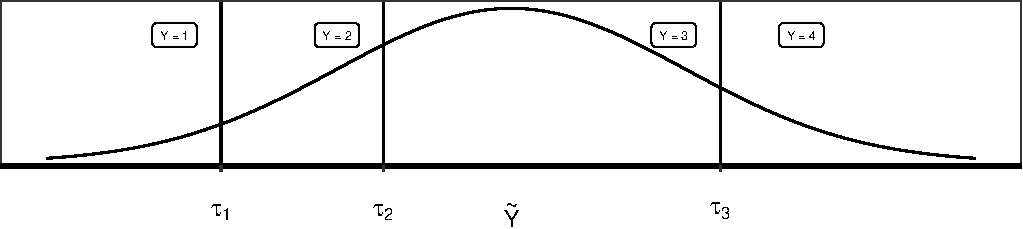
\includegraphics{2_files/figure-pdf/fig-cumulative-1.pdf}

}

\caption{\label{fig-cumulative}Función latente en una regresión ordinal
acumulativa.}

\end{figure}

Por ejemplo en la Figura~\ref{fig-cumulative},

\[Pr(Y = 2) = F(\tau_2) - F(\tau_{1})\]

Si suponemos que \(\tilde{Y}\) tiene una relación lineal los
predictores:

\[\tilde{Y} = \eta + \epsilon = \beta_1 x_1 + \beta_2 x_2 + ... + \beta_p x_p + \epsilon\]

entonces la función de probabilidad acumulada de los errores tendrá la
misma forma que la de \(\tilde{Y}\):

\[\mathrm{Pr}(\epsilon \leq z) = F(z)\]

Y podremos calcular la distribución de probabilidad acumulada de \(Y\):

\[\mathrm{Pr}(Y \leq k \mid \eta) = \mathrm{Pr}(\tilde{Y} \leq \tau_k \mid \eta) = \mathrm{Pr}(\eta + \epsilon \leq \tau_k) = \mathrm{Pr}(\epsilon \leq \tau_k - \eta) = F(\tau_k - \eta)\]

Por lo que asumiendo la normalidad de los errores:

\[\mathrm{Pr}(Y = k) = \Phi(\tau_k - \eta) - \Phi(\tau_{k - 1} - \eta)\]

Donde hay que estimar los umbrales y los coeficientes de regresión. La
función anterior es la conocida como la función de enlace
\texttt{probit}. Otra función de enlace popular es la función
\texttt{logit}. Es la que usaremos en este trabajo por ser más fácil su
interpretación \footnote{En la práctica los coeficientes estimados con
  las funciones de enlace \texttt{probit} y \texttt{logit} suelen
  similares.}. Con esta función de enlace la interpretación de los
coeficientes es parecida a la de los coeficientes de la regresión
logística. Para entender como se deben interpretar los coeficientes del
modelo \(CM\). se parte del supuesto de que el \(logit\) de la función
de probabilidad es lineal:

\begin{equation}\protect\hypertarget{eq-ordinal}{}{
logit [P(Y \le k)] = \tau_{k} - \eta = \tau_{k} - (\beta_1 x_1 + \beta_2 x_2 + ... + \beta_p x_p)
}\label{eq-ordinal}\end{equation}

En ese caso, se puede demostrar fácilmente que, por ejemplo:

\[\frac{\frac{\mathrm{Pr}(Y \leq k \mid \eta)}{\mathrm{Pr}(Y > k \mid \eta)}}{\frac{\mathrm{Pr}(Y \leq k+1 \mid \eta)}{\mathrm{Pr}(Y > k+1 \mid \eta)}} = \exp(\tau_{k} - \tau_{k+1})\]

Y que \footnote{En la Sección~\ref{sec-ordinal-2} se demuestra esta
  fórmula.}:

\[\frac{\frac{\mathrm{Pr}(Y \leq k \mid x_i = 1)}{\mathrm{Pr}(Y > k \mid x_i = 1)}}{\frac{\mathrm{Pr}(Y \leq k \mid x_i=0)}{\mathrm{Pr}(Y > k \mid x_i = 0)}} = \exp(-\beta_{i})\]

o, equivalentemente:

\[\frac{\frac{\mathrm{Pr}(Y > k \mid x_i = x + 1)}{\mathrm{Pr}(Y \leq k \mid x_i = x + 1)}}{\frac{\mathrm{Pr}(Y > k \mid x_i = x)}{\mathrm{Pr}(Y \leq k \mid x_i = x)}} = \exp(\beta_{i})\]

Es decir, que \(\exp(\beta_{i})\) es el \(OR\) (cambio relativo entre
\(odds\)) de que la variable respuesta esté por encima de una
determinada categoría versus estar por debajo de ella para una unidad de
incremento del predictor \(x_i\). Un valor del coeficiente \(\beta_i\)
positivo indica que la relación entre el predictor \(x_i\) y la función
de \(logit\) es positiva y, por lo tanto, se incrementa la probabilidad
de un mayor valor de la variable respuesta.

\hypertarget{asunciones-del-modelo}{%
\subsubsection{Asunciones del modelo}\label{asunciones-del-modelo}}

Este modelo se denomina proporcional ya que se asume que cada predictor
tiene los mismos efectos sobre todos los niveles de la variable de
respuesta ordinal \autocite[ver][]{Liu2202}. Es decir, que los \(odds\)
de los niveles de respuesta deben ser proporcionales para los mismos
valores de las variables explicativas. Esta suposición frecuentemente no
es realista y se puede relajar permitiendo estimar un coeficiente
diferente para cada nivel de la variable respuesta. Sin embargo, el
incremento del número de coeficientes dificulta la interpretabilidad del
modelo. \textcite{harrell2020} aboga por usar este modelo incluso aunque
la suposición de proporcionalidad no se cumpla:

\begin{quote}
\enquote{Ningún modelo se ajusta perfectamente a los datos, \ldots, la
aproximación ofrecida por el modelo \(CM\) sigue siendo bastante útil. Y
un análisis unificado del modelo \(CM\) es decididamente mejor que
recurrir a análisis ineficientes y arbitrarios de valores dicotomizados
de Y.}
\end{quote}

Matemáticamente la asunción de la proporcionalidad de los \(odd\) se
demuestra a partir de la Ecuación~\ref{eq-ordinal}. Si fijamos los
valores de los predictores en un valor arbitrario \(X=x\) y consideramos
dos niveles de respuesta cualesquiera \(k\) y \(l\), entonces:

\begin{equation}\protect\hypertarget{eq-ordinal2}{}{
\begin{aligned}
logit [P(Y \le k | X = x)] - logit [P(Y \le l | X = x)] & = \tau_{k} - \tau_{l} \\
\frac{odds(P(Y \le k | X = x))}{odds(P(Y \le l | X = x))} & =  \exp(\tau_{k} - \tau_{l}) \implies \\
odds(P(Y \le k | X = x)) & \propto odds(P(Y \le l | X = x))
\end{aligned}
}\label{eq-ordinal2}\end{equation}

Es decir, que la proporcionalidad de \(odds\) de dos niveles de
respuesta es independiente de los valores concretos de los predictores
por lo que la constante de proporcionalidad debe ser similar para todos
ellos. Esta proporcionalidad se puede comprobar mediante diferencia de
\(logits\).

\hypertarget{sec-multinivel}{%
\section{Modelos multinivel}\label{sec-multinivel}}

Un modelo multinivel, jerárquico o mixto es un modelo en el que los
datos están anidados en una estructura jerárquica. Por ejemplo, si se
quisiera evaluar el rendimiento de varios métodos de enseñanza, se
podrían seleccionar aleatoriamente varios colegios participantes y en
cada uno de ellos elegir varias clases en las que se impartiría uno de
los métodos de enseñanza. Los modelos multinivel se utilizan cuando se
incumple la hipótesis de independencia entre las observaciones. En el
caso de los métodos de enseñanza, los alumnos de una clase no son
independientes de los alumnos de otra clase del mismo colegio y también
es esperable que los alumnos de un mismo colegio sean más parecidos
entre sí que los de otro colegio. Otra situación en la que se viola la
condición de independencia entre observaciones es cuando se toman varias
medidas del mismo sujeto. Este tipo de experimentos se llaman de medidas
repetidas o longitudinales \footnote{Hay una diferencia conceptual entre
  medidas repetidas y longitudinales. Una variable se dice que es
  longitudinal cuando se toman varias medidas de los sujetos objeto del
  estudio en diferentes momentos del tiempo. Para que sea considerada de
  medidas repetidas, las medidas de cada sujeto se toman con distintos
  niveles de factor. En la práctica la distinción es poco relevante ya
  que ambas situaciones se parametrizan de la misma forma.}. Cuando se
da este supuesto, se considera que las medidas están anidadas en el
sujeto \autocite[ver][]{Liu2202}. En un modelo multinivel no es
necesario que todas las variables tengan una estructura jerárquica.
Distinguimos entonces dos tipos de variables: Las conocidas como de
efectos fijos son aquellas que se considera que tienen el mismo efecto
en toda la población y, por lo tanto, se debe estimar un único
coeficiente. Las variables de efectos aleatorios tienen un coeficiente
diferente para cada elemento de la población y se supone que son una
muestra de una población mucho mayor, como el caso de seleccionar
aleatoriamente una muestra de colegios. Normalmente el coeficiente
particular de cada elemento no es de interés para el investigador y se
asume que tienen una media centrada en cero. El mayor interés de los
efectos aleatorios es la estimación de su matriz de
varianzas-covarianzas.

La ecuación general de un modelo multinivel con dos niveles y un solo
predictor con efectos aleatorios es \autocite[ver][pp.~40]{chen2021}:

\[
\begin{aligned}
Level\ 1: & y_{ij}     & = & \beta_{0j} + \beta_{1j}x_{1ij} + \epsilon_{ij} \\
Level\ 2: & \beta_{0j} & = & \beta_{0} + U_{0j} & (intercepto\ aleatorio) \\
          & \beta_{1j} & = & \beta_{1} + U_{1j} & (pendiente\ aleatoria) \\
\end{aligned}
\]

donde los errores del modelo se distribuyen:

\[
\begin{aligned}
\text{Error intra grupo: } &  \epsilon_{ij} \sim N(0, \sigma^2) \\
\text{Error entre grupos: } &
\begin{pmatrix}
     U_{0j} \\
     U_{1j} \\
\end{pmatrix} 
\sim
N
\begin{pmatrix}
\begin{pmatrix}
     0 \\
     0 \\
\end{pmatrix},
\begin{pmatrix}
     \tau_0^2 & \tau_0\tau_1\rho_{01} \\
     \tau_0\tau_1\rho_{01} &  \tau_1^2 \\
\end{pmatrix}
\end{pmatrix} 
\end{aligned}
\]

donde \(j\) son los grupos que varían \(j = 1,...,J\) (\(J\) es el
número de grupos); \(ij\) es la observación \(i-ésima\) del grupo \(j\)
(\(i = 1,...,n_j\), \(n_j\) es el número de observaciones del grupo
\(j\)). El modelo se compone de una parte fija
\(\beta_0 + \beta_1 x_{1ij}\) y una aleatoria
\(U_{0j} + U_{1j} x_{1ij} + \epsilon{ij}\). Los parámetros de este
modelo son el intercepto y la pendiente de efectos fijos (\(\beta_0\) y
\(\beta_1\)), la varianza intra-grupos (\(\sigma^2\)), la varianza
inter-grupos del intercepto aleatoria (\(\tau_0\)) y de la pendiente
aleatoria (\(\tau_1\)), y la correlación entre intercepto y pendiente
aleatorias (\(\rho_{01}\)).

En \textcite{gelman2013} se evalúan tres posibilidades a la hora de
definir un modelo:

\begin{itemize}
\tightlist
\item
  \(Complete\ pooling\): Consiste en estimar un único parámetro para
  cada predictor. Es equivalente a un modelo con efectos fijos.
\item
  \(No\ pooling\): Se estiman tantos parámetros como grupos haya de
  forma independiente.
\item
  \(Partial\ pooling\): Es el modelo jerárquico. Es una mezcla de ambos,
  ya que aunque se estima un parámetro para cada grupo (como en
  \(no\ pooling\)), esta estimación no es independiente, sino que se
  supone que las observaciones de un mismo grupo proceden de una misma
  distribución de probabilidad. Esto se traduce en que se produce una
  contracción (\(shrinkage\)) en la estimación de los parámetros hacia
  la media. Al influir la estimación de unas observaciones en otras, la
  estimación es de menor valor absoluto que la que resultaría en un
  modelo de \(no\ pooling\). De esta forma podemos ver el
  \(complete\ pooling\) y el \(no\ pooling\) como dos casos particulares
  y extremos del \(partial\ pooling\). La contracción de coeficientes en
  los modelos multinivel actúa como una regularización que puede evitar
  el sobreajuste.
\end{itemize}

Los modelos multinivel requieren supuestos adicionales en el nivel
segundo y superiores que son similares a los supuestos para los modelos
de efectos fijos \autocite[ver][pp.~43]{chen2021}. Para estimar los
parámetros en un modelo multinivel se suele utilizar el método de máxima
verosimilitud restringida (RMLE), que es una variante de la estimación
por máxima verosimilitud (MLE) en la que se hacen ajustes en los grados
de libertad del modelo con efectos aleatorios para corregir el sesgo que
se produce al usar MLE en estos modelos.

\hypertarget{sec-bayesiano}{%
\section{Modelado bayesiano}\label{sec-bayesiano}}

El paradigma frecuentista parte de la suposición de que los datos son
generados a partir de una variable aleatoria \(Y\) y para estimar los
coeficientes se maximiza la función de verosimilitud
\(p(y \mid \theta)\) que depende del parámetro desconocido \(\theta\).
En el análisis bayesiano se considera que \(\theta\) es una variable
aleatoria ya que tenemos incertidumbre respecto a su valor. Esto se
traduce en que debemos asignar una distribución de probabilidad
\(p(\theta)\) conocida como distribución a priori que expresa nuestra
creencia sobre los valores que puede tomar \(\theta\). En la inferencia
bayesiana se usa la distribución de probabilidad a posteriori
\(p(\theta \mid y)\) que es proporcional al producto de la función de
verosimilitud y de la distribución de probabilidad a priori
\autocite[ver][]{nicenboim2023}:

\[
\hbox{Posterior} = \frac{\hbox{Likelihood} \times \hbox{Prior}}{\hbox{Marginal Likelihood}}
\Rightarrow p(\theta|y) = \cfrac{ p(y|\theta) \times p(\theta) }{p(y)} \propto p(y|\theta) \times p(\theta)
\]

En la inferencia bayesiana hay dos fuentes de incertidumbre: Por un lado
hay que contar con la variabilidad de \(Y\), ya que si se toman varias
muestras, los valores \(y_i\) obtenidos serán diferentes. Además, existe
otra incertidumbre que que proviene del desconocimiento del valor de
\(\theta\). En la estimación frecuentista, debido a que se utilizan
estimaciones puntuales de \(\theta\), no se tiene en cuenta esta
incertidumbre. La Ecuación~\ref{eq-ypred} se corresponde con la
distribución predictiva posteriori que tiene en consideración ambas
incertidumbres: \begin{equation}\protect\hypertarget{eq-ypred}{}{
\begin{aligned}
p(y_{pred}\mid y ) & = \int_{\theta} p(y_{pred}, \theta \mid y)\, d\theta= \int_{\theta} 
p(y_{pred}\mid \theta,y)p(\theta \mid y)\, d\theta \\ 
& = \int_{\theta} p(y_{pred}\mid \theta) p(\theta \mid y)\, d\theta
\end{aligned}
}\label{eq-ypred}\end{equation}

donde la última igualdad resulta de la independencia condicional de
\(y_{pred}\) e \(y\) dado \(\theta\)
(\(y_{pred} \perp\!\!\!\perp y \mid \theta\)). Una crítica habitual a la
inferencia bayesiana es que la elección de la distribución de
probabilidad a priori es subjetiva. Aunque es cierto que hay un grado de
subjetividad en esta elección, en realidad en el modelado frecuentista
hay que tomar ciertas decisiones que también lo son, como por ejemplo la
elección del nivel de significación o la forma que adopta la función de
verosimilitud. En la práctica, si las observaciones son suficientemente
informativas y la distribución a priori es poco informativa, la
distribución de probabilidad a priori tendrá poca o nula influencia en
la distribución a posteriori ya que estará dominada por la función de
verosimilitud y los coeficientes estimados serán muy parecidos en ambos
paradigmas. Sin embargo, en lo que diferirán es en la interpretación ya
que, por ejemplo, en un modelo bayesiano se pueden interpretar los
intervalos de confianza como la probabilidad de que el parámetro esté
dentro del intervalo \footnote{Por eso a estos intervalos se les conoce
  como intervalos de credibilidad.}. Esa interpretación en un modelo
frecuentista carecería de sentido ya que los parámetros del modelo no se
consideran variables aleatorias y, por lo tanto, tendrán probabilidad 1
si el verdadero valor del parámetro cae dentro del intervalo y 0 si no
lo hace. Para obtener la distribución de probabilidad a posteriori
normalmente se recurre a métodos del simulación MCMC (Métodos de
Montcarlo basados en Cadenas de Márkov) \footnote{En ocasiones se puede
  obtener una forma análitica de la distribución a posteriori si se
  elige una adecuada combinación de función de verosimilitud y
  distribución a priori conocidas como distribuciones conjugadas. Aunque
  esto evita la utilización de métodos de simulación, restringe las
  formas posibles de las distribuciones. En la actualidad, con el
  aumento de la capacidad de cálculo de los ordenadores, normalmente no
  es necesaria la utilización de distribuciones conjugadas.}.

Para comparar modelos entre sí se pueden usar varias medidas
\autocite[ver][]{barreda2023}. Por ejmplo, la conocida como \emph{log
pointwise predictive density} o densidad predictiva puntal (\(lpd\)) se
puede calcular: \[
\widehat{\mathrm{lpd}} = \sum_{i=1}^{N} \mathrm{log} (p(y_{i} | \theta))
\]

La \(lpd\) es la densidad conjunta de observar los datos dada la
estructura del modelo y las estimaciones de los parámetros \(\theta\).
Aunque las probabilidades a priori no se incluyen en su cálculo, sí
influyen en la estimación de \(\theta\) y, por lo tanto, tienen un
efecto en los valores de \(lpd\). Mayores valores de \(lpd\) estarían
indicando un mejor modelo. El problema con esta métrica es que se
utilizan los datos tanto para estimar el modelo como para seleccionar el
mejor modelo. Esto va a producir un sobreajuste y tenderá a favorecer
los modelos más complejos. Una métrica mejor es la \emph{expected log
pointwise predictive density} o densidad predictiva puntual esperada
(\(elpd\)). Se define en términos de valores fuera de la muestra
\(\tilde{y}\) en lugar de con los valores de la muestra \(y\):

\[
\mathrm{elpd} = \sum_{i=1}^{N} \mathbb{E}(\mathrm{log} (p(\tilde{y}_i | \theta)))
\]

En la práctica no podemos saber el valor de \(elpd\) ya que no conocemos
el proceso que genera verdaderos valores \(\tilde{y}\). Una forma de
estimar \(elpd\) que empíricamente se ha visto que funciona es penalizar
\(lpd\) con el número de parámetros \(p\) de formá análoga a los que se
hace en \(AIC\) (ver Ecuación~\ref{eq-aic}):

\[
\widehat{\mathrm{elpd}} = \widehat{\mathrm{lpd}} - \mathrm{p}
\]

El problema es que en modelos multinivel conocer el número de parámetros
no es sencillo ya que los parámetros asociados a efectos aleatorios no
se pueden considerar que sean completamente independientes. El número
efectivo de parámetros va a depender de la importancia de la regresión
hacia la media que sufra cada parámetro. Además, en lugar de usar una
estimación puntual, se puede utilizar toda la distribución de valores de
la simulación. La métrica \emph{widely available information criterion}
o \enquote{criterio de información ampliamente disponible} (\(WAIC\)) es
una forma de estimar \(lpd\) que usa toda la distribución de
probabilidad a posteriori:

\[
\widehat{\mathrm{lpd}} = \sum_{i=1}^{n} \mathrm{log} (\frac{1}{S} \sum_{s=1}^{S} p(y_{i} | \theta^s))
\]

donde \(S\) es el tamaño de la muestra y el sumatorio interior es la
media de densidad en un punto \(i\). Para penalizar los modelos más
complejos, se usa la varianza de la función de densidad logarítmica:

\[
\begin{aligned}
\widehat{\mathrm{elpd}}_{WAIC} &= \widehat{\mathrm{lpd}} - \mathrm{p_{WAIC}} \\
\mathrm{p_{\mathrm{WAIC}}} &= \sum_{i=1}^{n} \mathrm{Var}_{s=1}^{\,S}(\mathrm{log} (p(y_{i} | \theta^s)))
\end{aligned}
\]

Una forma alternativa de evaluar un modelo es mediante validación
cruzada. Para evitar tener que dividir el conjunto de datos en datos de
entrenamiento y de validación se puede hacer validación cruzada de un
solo elemento o \(LOO\). En esta validación se deja un elemento fuera
cada vez. El problema es que tendremos que estimar el modelo tantas
veces como datos tengamos. Para evitar esto, hay formas de aproximar
\(\widehat{\mathrm{elpd}}\) basadas en \(LOO\) sin tener que reentrenar
el modelo. Las fórmula es la siguiente:

\[
\begin{aligned}
\widehat{\mathrm{elpd}}_{LOO} \approx \sum_{i=1}^{n} \mathrm{log} (p(y_{i} | \theta_{y_{-i}}))
\end{aligned}
\]

donde \(\theta_{y_{-i}}\) es la estimación de \(\theta\) que resulta
tras eliminar la observación \(y_{i}\) \footnote{No se entra en detalles
  de como estimar \(\theta_{y_{-i}}\) sin reentrenar el modelo.}.

\bookmarksetup{startatroot}

\hypertarget{sec-metodo}{%
\chapter{Métodología/Materiales y métodos}\label{sec-metodo}}

\hypertarget{descripciuxf3n-de-la-experiencia}{%
\section{Descripción de la
experiencia}\label{descripciuxf3n-de-la-experiencia}}

\hypertarget{marco-de-la-experiencia}{%
\subsection{Marco de la experiencia}\label{marco-de-la-experiencia}}

Los datos se recogieron de una actividad de subtitulado que se propuso a
los estudiantes de la edición 2022 del curso MOOC Materiales digitales
accesibles de la UNED Abierta. Este curso pertenece al Canal Fundación
ONCE (IEDRA) está dirigido por los profesores Emilio Letón Molina y
Alejandro Rodríguez Ascaso y según se recoge en la propia página Web del
curso sus objetivos son:

\begin{itemize}
\item
  Reconocer y abordar los desafíos a los que se enfrentan las personas
  con discapacidad (por ejemplo los estudiantes) al usar los documentos
  electrónicos, adquirir conciencia y experiencia.
\item
  Obtener una mejor comprensión de la accesibilidad como un asunto de
  derechos civiles y desarrollar los conocimientos y habilidades
  necesarios para diseñar recursos de aprendizaje que promuevan
  ambientes de aprendizaje inclusivos.
\item
  Valorar cómo los documentos accesibles benefician a todas las
  personas, incluyendo a las que tienen y a las que no tienen
  discapacidad, a través de una mayor facilidad de uso y la
  interoperabilidad de los materiales basados en la web.
\item
  Tomar conciencia de que cómo los autores pueden no solo eliminar
  barreras, sino evitar crearlas en primer lugar.
\item
  Adquirir autosuficiencia en la producción de contenidos accesibles y
  en la identificación de problemas de accesibilidad.
\item
  Adquirir, como autores, estrategias para la producción sostenible de
  material digital, como la modularidad.
\end{itemize}

Está destinado \enquote{a todos aquellas personas que desean participar
en el desarrollo de soluciones de diseño éticas y creativas, que quieran
escribir o gestionar contenidos electrónicos accesibles, desde páginas
web o aplicaciones a libros electrónicos}ePub''.

El curso tiene cuatro módulos:

\begin{itemize}
\tightlist
\item
  Introducción.
\item
  Accesibilidad de material multimedia.
\item
  Accesibilidad de texto digitales.
\item
  Materiales digitales en la práctica.
\end{itemize}

\hypertarget{actividad-de-subtitulado}{%
\subsection{Actividad de subtitulado}\label{actividad-de-subtitulado}}

La actividad de subtitulado es voluntaria y sin influencia en la
calificación final del alumno ni el material al que se tiene acceso. Se
realiza en el módulo \enquote{Accesibilidad del material multimedia}. En
este mismo módulo, y antes de proponerles la actividad de subtitulado,
los alumnos completaron las secciones \enquote{Accesibilidad de la
información sonora} y \enquote{Accesibilidad de la información visual},
con lo cual ya tienen conocimiento sobre creación de vídeos y subtítulos
accesibles.

La actividad consistió en ver dos vídeos idénticos y que solo se
diferencian en la calidad del subtitulado de 43 segundos de duración.
Los subtítulos de uno de los vídeos se realizaron
\autocites[ver][]{jperez1,jperez2} siguiendo la guía Web Content
Accessibility Guidelines 2.1 (WCAG 2.1) del W3C (World Wide Web
Consortium). El otro vídeo tenía un subtitulado similar pero se
introdujeron pequeñas deficiencias, algunas de ellas inapreciables para
alguien que carezca de conocimientos sobre accesibilidad. El orden de
los vídeos es aleatorio, de tal forma que una cohorte de alumnos vio
primero el vídeo bien subtitulado y luego el mal subtitulado y la otra
lo hizo al revés. Después de ver cada uno de los vídeos, los alumnos
respondieron a una escala de Likert de 5 niveles y 18 ítems. Los 18
items de Likert responden a los criterios de la norma UNE 153010
\autocite[ver][]{aenor2012}. El diseño de experimento es doble ciego: es
decir, a los alumnos no se les informó de si estaban viendo el vídeo con
mejor o con peor calidad de subtitulado. Esta información tampoco se
conoce en el momento de realizar este trabajo ya que los vídeos tienen
identificaciones genéricas que no contienen ninguna indicación del tipo
de subtitulado del vídeo\footnote{En la respuesta a cada ítem, el alumno
  puede añadir comentarios. Éstos han sido eliminados del estudio para
  que no filtren información referente al tipo de subtitulado que el
  alumno cree estar contestando.}.

En la Tabla~\ref{tbl-likert-levels} se muestran los 5 niveles de cada
uno de los items de la escala de Likert utilizados para valorar el
subtitulado \footnote{En la codificación original los valores asignados
  a cada respuesta eran diferentes: la opción \enquote{No sé / No
  contesto} se codificó con 5 y las demás opciones con una unidad menos
  que la mostrada. En este trabajo se ha hecho una rotación para asignar
  valores más usuales en la literatura científica sobre el tema.}. En la
Tabla~\ref{tbl-likert-scale} se muestran los 18 items de la escala de
Likert que se propuso a los alumnos para que evaluaran cada uno de los
vídeos.

\hypertarget{tbl-likert-levels}{}
\begin{longtable}[]{@{}rl@{}}
\caption{\label{tbl-likert-levels}Niveles de los items de la escala de
Likert.}\tabularnewline
\toprule\noalign{}
values & levels \\
\midrule\noalign{}
\endfirsthead
\toprule\noalign{}
values & levels \\
\midrule\noalign{}
\endhead
\bottomrule\noalign{}
\endlastfoot
0 & No sé / No contesto \\
1 & Muy en desacuerdo \\
2 & En desacuerdo \\
3 & Neutral \\
4 & De acuerdo \\
5 & Muy de acuerdo \\
\end{longtable}

\hypertarget{tbl-likert-scale}{}
\begin{longtable}{ll}
\caption{\label{tbl-likert-scale}Items de la escala de Likert. }\tabularnewline

\toprule
Item & Texto \\ 
\midrule
Q01 & La posición de los subtítulos. \\ 
Q02 & El número de líneas por subtítulo. \\ 
Q03 & La disposición del texto respecto a la caja donde se muestran los subtítulos. \\ 
Q04 & El contraste entre los caracteres y el fondo. \\ 
Q05 & La corrección ortográfica y gramatical. \\ 
Q06 & La literalidad. \\ 
Q07 & La identificación de los personajes. \\ 
Q08 & La asignación de líneas a los personajes en los diálogos. \\ 
Q09 & La descripción de efectos sonoros. \\ 
Q10 & La sincronización de las entradas y salidas de los subtítulos. \\ 
Q11 & La velocidad de exposición de los subtítulos. \\ 
Q12 & El máximo número de caracteres por línea. \\ 
Q13 & La legibilidad de la tipografía. \\ 
Q14 & La separación en líneas diferentes de sintagmas nominales, verbales y preposicionales. \\ 
Q15 & La utilización de puntos suspensivos. \\ 
Q16 & La escritura de los números. \\ 
Q17 & Las incorrecciones en el habla. \\ 
Q18 & Los subtítulos del vídeo cumplen en general con los requisitos de accesibilidad. \\ 
\bottomrule
\end{longtable}

\hypertarget{participantes}{%
\section{Participantes}\label{participantes}}

Los datos personales de los estudiantes se suministraron anonimizados
para evitar conocer su identidad. De acuerdo con nuestro compromiso
ético, del estudio se han eliminado a aquellos estudiantes que, a pesar
de haber realizado la actividad, no dieron su consentimiento para que
sus datos se utilizaran en estudios científicos. Tras este proceso, se
dispone de 198 cuestionarios correspondientes a 111 alumnos. Hay 24
estudiantes que sólo realizaron el primero de los test. Como la muestra
es suficientemente amplia, se ha decidido eliminar estos test quedando
87 estudiantes participantes. En la Tabla~\ref{tbl-contingencia-eco} se
muestran las tablas de contingencia de algunos de los datos que los
estudiantes voluntariamente facilitaron en el cuestionario inicial del
curso.

\begin{table}

\caption{\label{tbl-contingencia-eco}Tablas de contingencia de la
información del sexo, edad y nivel de conocimientos
previos.}\begin{minipage}[t]{0.50\linewidth}

{\centering 

\hypertarget{tbl-contingencia-eco-1}{}
\begin{longtable}{cr}
\tabularnewline

\toprule
gender & Freq \\ 
\midrule
femenino & 46 \\ 
masculino & 19 \\ 
NA & 22 \\ 
\bottomrule
\end{longtable}

Estudiantes por sexo.

}

\end{minipage}%
%
\begin{minipage}[t]{0.50\linewidth}

{\centering 

\hypertarget{tbl-contingencia-eco-2}{}
\begin{longtable}{cr}
\tabularnewline

\toprule
year\_of\_birth & Freq \\ 
\midrule
None & 22 \\ 
NA & 1 \\ 
\bottomrule
\end{longtable}

Estudiantes con valor nulo en el campo año de nacimiento.

}

\end{minipage}%
\newline
\begin{minipage}[t]{0.50\linewidth}

{\centering 

\hypertarget{tbl-contingencia-eco-3}{}
\begin{longtable}{cr}
\tabularnewline

\toprule
level\_of\_knowledge & Freq \\ 
\midrule
4 & 1 \\ 
6 & 2 \\ 
7 & 15 \\ 
8 & 22 \\ 
9 & 20 \\ 
10 & 16 \\ 
NA & 11 \\ 
\bottomrule
\end{longtable}

Estudiantes en función del número de preguntas acertadas en el test de
conocimiento sobre accesibilidad.

}

\end{minipage}%

\end{table}

\hypertarget{ficheros-suministrados}{%
\section{Ficheros suministrados}\label{ficheros-suministrados}}

Se dispuso de los siguientes ficheros \texttt{csv}:

\begin{itemize}
\tightlist
\item
  El fichero \texttt{grade} contiene el identificador de estudiante y el
  grupo al que pertenece (campo \texttt{cohort}).
\item
  El fichero \texttt{abo} es la información socioeconómica que
  voluntariamente ha aportado el estudiante: sexo, año nacimiento, nivel
  de estudios, ocupación.
\item
  El fichero \texttt{conoc} contiene el test de evaluación inicial de
  conocimientos del estudiante.
\item
  El fichero \texttt{exp} es la evaluación del curso realizada por cada
  estudiante.
\item
  El fichero \texttt{acc} contiene la información sobre las
  necesidades/preferencias de accesibilidad que tiene el estudiante.
\item
  Los ficheros \texttt{test1} y \texttt{test2} son las repuestas a las
  escalas de Likert sobre la calidad del subtitulado del primer y del
  segundo vídeo realizado por cada grupo respectivamente.
\end{itemize}

\hypertarget{sec-preprocesado}{%
\section{Preprocesado}\label{sec-preprocesado}}

En esta sección se describen las transformaciones realizadas con los
ficheros suministrados:

\begin{itemize}
\item
  Se lee el fichero de perfil del usuario. El número de fila con el que
  el usuario aparece en el fichero se utilizará como identificador del
  usuario para mantener la trazabilidad y comprobar que las
  transformaciones realizadas son correctas.
\item
  Se eliminan los datos de los estudiantes que, aun habiendo realizado
  la actividad, no han dado su consentimiento para participar en el
  estudio.
\item
  El valor del campo \texttt{cohort} se sustituye por una letra, \(A\) o
  \(B\), en función del grupo asignado. En el momento de realizar este
  proceso se desconoce qué vídeo vio primero cada cohorte.
\item
  Se lee el fichero \texttt{profile} y se añade información sobre el
  sexo y el año de nacimiento.
\item
  Se lee el fichero \texttt{conoc} y se calcula cuántas preguntas acertó
  cada usuario en el test de evaluación de conocimientos previos. Se
  añade esta información al perfil del usuario.
\item
  Se leen los ficheros de test y se procesan. Se utiliza el nombre del
  fichero (\texttt{test1} o \texttt{test2}) para saber de qué vídeo se
  está respondiendo el test \footnote{Se reitera que en el momento de
    realizar este proceso se desconoce si el vídeo es el correctamente
    subtitulado o el otro. La única información que se almacena es si se
    está respondiendo al vídeo que se vio primero.}.
\item
  Se seleccionan las preguntas que contienen las respuestas y se
  renombran para que sea más fácil saber de qué pregunta se trata
  \footnote{En los ficheros suministrados la respuesta a cada pregunta
    ocupa varios campos. Se selecciona en cada pregunta el que contiene
    el valor de la respuesta y se convierte a numérico.}. Se convierte
  el campo \texttt{LastTry}, que contiene la fecha y hora de realización
  del test, a formato fecha y hora.
\item
  Se realizan algunas comprobaciones como la ausencia de valores nulos
  en la variables más relevantes o que no existan inconsistencias ni
  errores de procesado.
\item
  Se eliminan los comentarios y se graban en fichero aparte para que no
  revelen información que podría descubrir el tipo de subtitulado que
  piensa que está evaluando el estudiante.
\item
  Se almacenan los resultados de los test preprocesados en un fichero
  \texttt{csv}.
\end{itemize}

\hypertarget{variables}{%
\section{Variables del modelo.}\label{variables}}

En la Tabla~\ref{tbl-variables} se describen las características más
relevantes de las principales variables que se utilizarán en el modelado
y en el análisis estadístico.

\footnotesize

\hypertarget{tbl-variables}{}
\setlength{\LTpost}{0mm}
\begin{longtable}{llll}
\caption{\label{tbl-variables}Descripción de las variables más importantes. }\tabularnewline

\toprule
Nombre & Descripción & Tipo & Valores \\ 
\midrule
Response & Respuesta a las preguntas del test. & Factor ordenado & De 0 a 5\textsuperscript{\textit{1}} \\ 
Level & Valoración de la respuesta. & Factor ordenado & Negative, Neutral, Positive\textsuperscript{\textit{2}} \\ 
Treat & Subtítulos & Factor & A o B\textsuperscript{\textit{3}} \\ 
Period & Periodo & Factor & 1 ó 2\textsuperscript{\textit{4}} \\ 
Seq & Secuencia de aplicación de los tratamientos. & Factor & AB o BA \\ 
Subject & Identificación del estudiante & Factor & Numérico \\ 
Question & Número de la pregunta & Factor & Q01, Q02, ..., Q18\textsuperscript{\textit{5}} \\ 
\bottomrule
\end{longtable}
\begin{minipage}{\linewidth}
\textsuperscript{\textit{1}}Se ha hecho una rotación sobre los valores originales. 0 = No sé, 1 = Muy en desacuerdo, ..., 5 Muy de acuerdo.\\
\textsuperscript{\textit{2}}Positive cuando Response sea 4 ó 5, Negative cuando sea 1 ó 2 y Neutral para 3.\\
\textsuperscript{\textit{3}}No se conoce si el tratamiento A es el subtitulado bueno o lo es el B.\\
\textsuperscript{\textit{4}}1 para el primer vídeo visto y 2 el segundo.\\
\textsuperscript{\textit{5}}Se ha reorganizado de tal forma que Q18, que es la pregunta resumen, sea el valor primero y de referencia.\\
\end{minipage}

\normalsize

Partiendo del \texttt{dataframe} que se construyó en el preprocesado
(ver Sección~\ref{sec-preprocesado}) construimos el \texttt{dataframe}
que usaremos a partir de este momento. Las operaciones principales que
se han realizado han sido:

\begin{itemize}
\tightlist
\item
  Renombrar las variables (ver Tabla~\ref{tbl-variables}).
\item
  Eliminar del estudio los usuarios que solo han realizado uno de los
  test.
\item
  Transformar las variables que lo requieran en factores. La pregunta 18
  se usará como referencia en el factor \texttt{Question}.
\item
  Rotar los valores de respuesta para que \enquote{No sé / No contesto}
  tenga valor 0 y el resto de 1 a 5 desde \enquote{Muy en desacuerdo},
  1, hasta \enquote{Muy de acuerdo}, 5.
\item
  Crear el factor \texttt{Level} con los niveles \texttt{negative},
  \texttt{neutral} y \texttt{positive} dependiendo de si la respuesta es
  1 ó 2, 3, 4 ó 5 respectivamente.
\item
  Transformar el \texttt{dataframe} de formato ancho a largo: los
  ficheros de respuestas se suministran en formato ancho. Es decir, que
  cada fila es un test que contiene 18 columnas para las respuestas a
  cada pregunta. Los nombres de las columnas son \(Q01\), \(Q02\),
  \ldots, \(Q18\) y tendrán valores de 0 a 5 con las respuestas. La
  mayoría de los paquetes de R que vamos a usar requieren que los datos
  estén en formato largo. Esto que quiere decir que cada fila tendrá una
  única respuesta por lo que habrá únicamente dos columnas, \(Question\)
  y \(Response\). En la primera se almacenará el identificador de la
  pregunta (\(Q01\), \(Q02\), \ldots, \(Q18\)) y en la segunda el valor
  de la respuesta (de 0 a 5). De esta forma, un test pasará de ocupar
  una fila y 18 columnas en el formato ancho a 18 filas y dos columnas
  en el largo.
\end{itemize}

Se crean dos \texttt{dataframes}:

\begin{itemize}
\tightlist
\item
  \texttt{df\_all} contiene en formato largo todas las respuestas a los
  test.
\item
  \texttt{df\_clean} tiene la misma estructura que \texttt{df\_all} pero
  en él se han eliminado las respuestas \enquote{No sé / No contesto}.
\end{itemize}

\texttt{df\_all} se utilizará cuando se traten las respuestas como
categóricas y, por lo tanto, como no ordenadas. \texttt{df\_clean} se
utilizará cuando se traten las respuestas como ordenadas y por ello no
contiene las respuestas con valor \enquote{No sé / No contesto}.

La estructura de estos \texttt{dataframes} es la siguiente:

\begin{verbatim}
tibble [2,980 x 7] (S3: tbl_df/tbl/data.frame)
 $ Seq     : Factor w/ 2 levels "AB","BA": 1 1 1 1 1 1 1 1 1 1 ...
 $ Period  : Factor w/ 2 levels "1","2": 1 1 1 1 1 1 1 1 1 1 ...
 $ Treat   : Factor w/ 2 levels "A","B": 1 1 1 1 1 1 1 1 1 1 ...
 $ Subject : Factor w/ 87 levels "4","33","35",..: 1 1 1 1 1 1 1 1 1 1 ...
 $ Question: Factor w/ 18 levels "Q18","Q01","Q02",..: 1 2 3 4 5 6 7 8 9 10 ...
 $ Response: Ord.factor w/ 5 levels "1"<"2"<"3"<"4"<..: 3 3 3 3 3 3 3 3 3 3 ...
 $ Level   : Ord.factor w/ 3 levels "Negative"<"Neutral"<..: 2 2 2 2 2 2 2 2 2..
\end{verbatim}

En la Tabla~\ref{tbl-df_clean} se muestran algunos ejemplos datos.

\hypertarget{tbl-df_clean}{}
\begin{longtable}{ccccccc}
\caption{\label{tbl-df_clean}Muestra del dataframe preparado para el modelado estadístico en formato
largo. }\tabularnewline

\toprule
Seq & Period & Treat & Subject & Question & Response & Level \\ 
\midrule
BA & 1 & B & 333 & Q13 & 4 & Positive \\ 
AB & 2 & B & 498 & Q13 & 4 & Positive \\ 
BA & 1 & B & 986 & Q16 & 3 & Neutral \\ 
AB & 2 & B & 1011 & Q08 & 2 & Negative \\ 
BA & 1 & B & 1118 & Q14 & 4 & Positive \\ 
AB & 2 & B & 75 & Q11 & 5 & Positive \\ 
AB & 2 & B & 1117 & Q11 & 4 & Positive \\ 
AB & 1 & A & 1011 & Q11 & 5 & Positive \\ 
AB & 1 & A & 288 & Q13 & 4 & Positive \\ 
AB & 2 & B & 288 & Q14 & 2 & Negative \\ 
\bottomrule
\end{longtable}

\bookmarksetup{startatroot}

\hypertarget{sec-modelado}{%
\chapter{Modelado estadístico}\label{sec-modelado}}

En este capítulo se realizará un análisis inicial para describir los
datos y descubrir las relaciones que se han encontrado utilizando
técnicas de estadística descriptiva. En la
Sección~\ref{sec-modelos-utilizados} se concreta y detalla cómo se
aplicarán las técnicas estadísticas propuestas en el
Capítulo~\ref{sec-arte} al diseño de experimento. Se pospone la
presentación de resultados al Capítulo~\ref{sec-resultados}.

\hypertarget{sec-eda}{%
\section{Análisis inicial}\label{sec-eda}}

Como se explica en la Tabla~\ref{tbl-variables}, al subtitulado le
denominamos tratamiento y a sus niveles (correcto e incorrecto) se les
ha llamado \(A\) y \(B\) sin hacer ninguna conjetura de cual de los dos
es el subtitulado correcto. El grupo con secuencia \(AB\) será el que
primero vio el vídeo con subtitulado \(A\) y luego el \(B\).
Análogamente, el grupo con secuencia \(BA\) vio los vídeos en orden
inverso. Recuérdese que el nivel 0 de respuesta se corresponde con
\enquote{No sé / No contesto} (ver Tabla~\ref{tbl-likert-levels}). Tras
eliminar los test de los usuarios que no dieron su consentimiento para
participar en el estudio y los de los que no realizaron el segundo test,
las dos cohortes están equilibradas (ver Figura~\ref{fig-groups}).

\begin{figure}[h]

{\centering 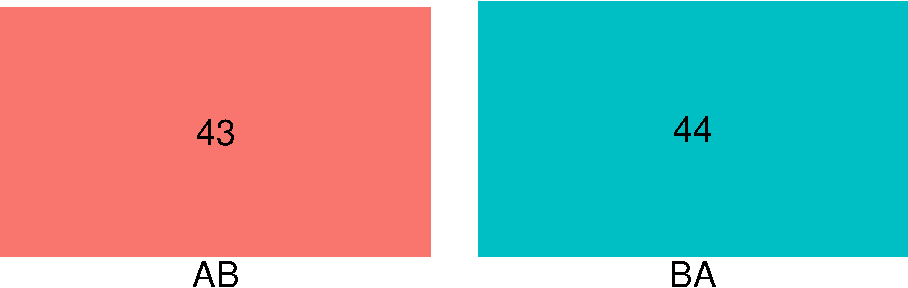
\includegraphics{4_files/figure-pdf/fig-groups-1.pdf}

}

\caption{\label{fig-groups}Estudiantes asignados a cada grupo.}

\end{figure}

\hypertarget{anuxe1lisis-de-la-calidad-de-los-datos}{%
\subsection{Análisis de la calidad de los
datos}\label{anuxe1lisis-de-la-calidad-de-los-datos}}

En esta sección se analiza si hay test que tienen valores de respuesta
que puedan resultar anómalos. En los test no se ha observado ningún
valor nulo ni erróneo.

El campo \texttt{LastTry} contiene la fecha y hora de realización del
test. Con esta información se puede conocer el tiempo que empleó cada
estudiante entre actividades. La Tabla~\ref{tbl-washout} muestra que hay
algunos test que se hicieron demasiado rápido \footnote{Hay que tener en
  cuenta que la duración de vídeo es de algo más de 40 segundos y que
  los estudiantes tienen que contestar un test de 18 ítems.}.

\hypertarget{tbl-washout}{}
\begin{longtable}{c}
\caption{\label{tbl-washout}Tiempos de realización de la segunda actividad de duración inferior a 2
minutos. }\tabularnewline

\toprule
Minutes \\ 
\midrule
0.93 \\ 
1.3 \\ 
1.7 \\ 
1.72 \\ 
1.78 \\ 
1.97 \\ 
\bottomrule
\end{longtable}

La Figura~\ref{fig-distinct} muestra que hay 28 test en los que el
estudiante contestó a todos los ítems usando únicamente 2 respuestas
diferentes. Además hay 13 test en los que se contestaron todas los ítems
con 1 respuesta.

\begin{figure}[h]

{\centering 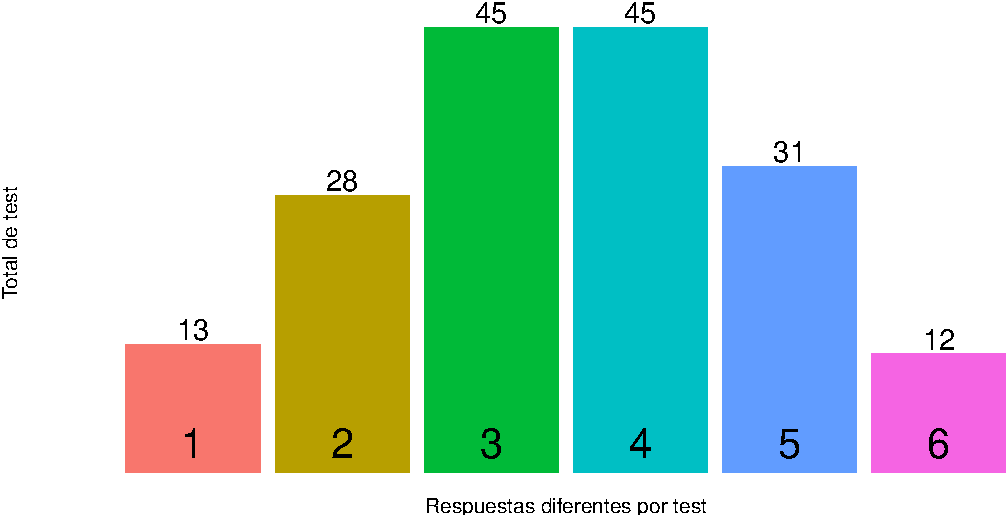
\includegraphics{4_files/figure-pdf/fig-distinct-1.pdf}

}

\caption{\label{fig-distinct}Número de respuestas diferentes en un mismo
test.}

\end{figure}

La tabla Tabla~\ref{tbl-distinct2} muestra los test de respuesta única y
el valor de esa respuesta.

\hypertarget{tbl-distinct2}{}
\begin{longtable}{rlr}
\caption{\label{tbl-distinct2}Test en los que todas las preguntas se contestan el mismo valor de
respuesta. }\tabularnewline

\toprule
Response & Seq & Test \\ 
\midrule
2 & AB & 01 \\ 
2 & AB & 02 \\ 
3 & BA & 01 \\ 
3 & BA & 02 \\ 
3 & BA & 02 \\ 
3 & BA & 02 \\ 
4 & AB & 01 \\ 
4 & AB & 01 \\ 
4 & AB & 02 \\ 
4 & BA & 01 \\ 
4 & BA & 02 \\ 
4 & BA & 02 \\ 
4 & BA & 02 \\ 
\bottomrule
\end{longtable}

La Figura~\ref{fig-compare} presenta la distribución de la cantidad de
respuestas cuyo valor cambia entre los dos test que realiza cada
estudiante.

\begin{figure}[h]

{\centering 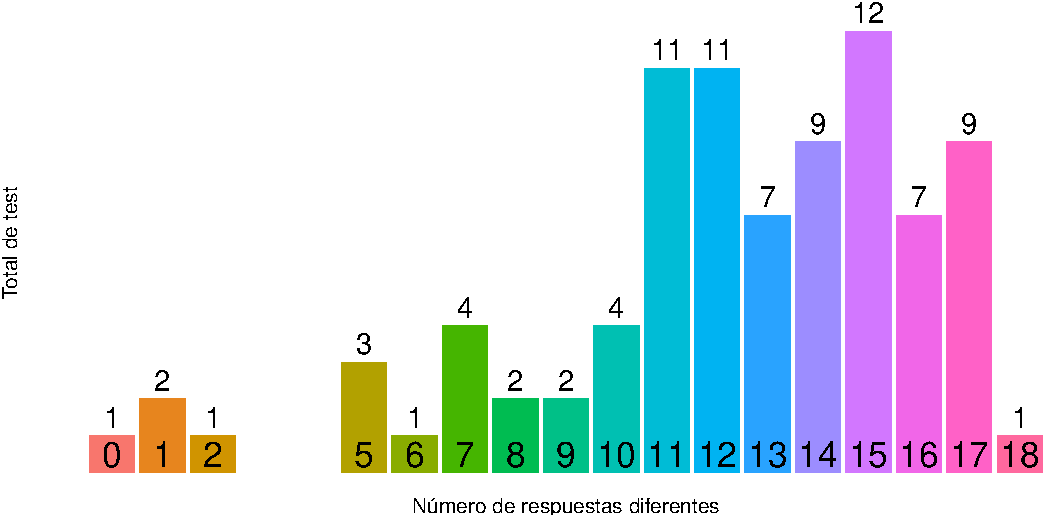
\includegraphics{4_files/figure-pdf/fig-compare-1.pdf}

}

\caption{\label{fig-compare}Número de respuestas diferentes entre los
test para cada estudiante.}

\end{figure}

Tan solo 1 estudiante respondió a todas las preguntas con el mismo valor
en los dos test. Por otro lado, no hay test que tengan un número
excesivo de contestaciones \enquote{No sé/No contesto} (ver
Tabla~\ref{tbl-noanswer}).

\hypertarget{tbl-noanswer}{}
\begin{longtable}{rr}
\caption{\label{tbl-noanswer}Los 5 test con más respuestas `No sé/No contesto' }\tabularnewline

\toprule
Test & Total respuesta por test \\ 
\midrule
01 & 5 \\ 
01 & 5 \\ 
02 & 5 \\ 
02 & 5 \\ 
01 & 4 \\ 
\bottomrule
\end{longtable}

Vemos que algunos test tienen valores que no parecen muy razonables. Por
ejemplo, no parece razonable realizar la actividad en menos de 2
minutos. Se observa que en algunos test hay poca variabilidad. Sin
embargo, no son muchos los test con estas características así que se ha
decidido mantener estos datos a pesar de que se pueda dudar de si en
ellos los estudiantes contestaron con la debida atención y diligencia.

\hypertarget{sec-eda-3}{%
\subsection{\texorpdfstring{Comparación de los tratamientos \(A\) y
\(B\) entre
grupos.}{Comparación de los tratamientos A y B entre grupos.}}\label{sec-eda-3}}

La Figura~\ref{fig-diff} presenta una forma de comparar los dos test
realizados por los estudiantes. Para cada estudiante se comparó pregunta
a pregunta sus dos test y se contabilizó la diferencia entre el número
de preguntas en que la puntuación en el segundo vídeo fue superior y en
las que lo fue inferior (las que no variaron de puntuación no se
consideraron). En el eje \(x\) se muestra la diferencia entre preguntas.
Cantidades negativas indican que hay más respuestas en el segundo de los
test que han empeorado respecto al primero de las que han mejorado. En
el eje \(y\) se representa el número de estudiantes para cada
diferencia. Esta frecuencia se representa en negativo cuando la
diferencia es negativa \footnote{En la comparación se han omitido
  aquellas respuestas en las que el estudiante contestó \enquote{No
  sé/No contesto} en la pregunta correspondiente de uno de los test.}.
Esto es una forma de evaluar si el estudiante valoró mejor o no el
segundo vídeo que el primero.

\begin{figure}[h]

{\centering 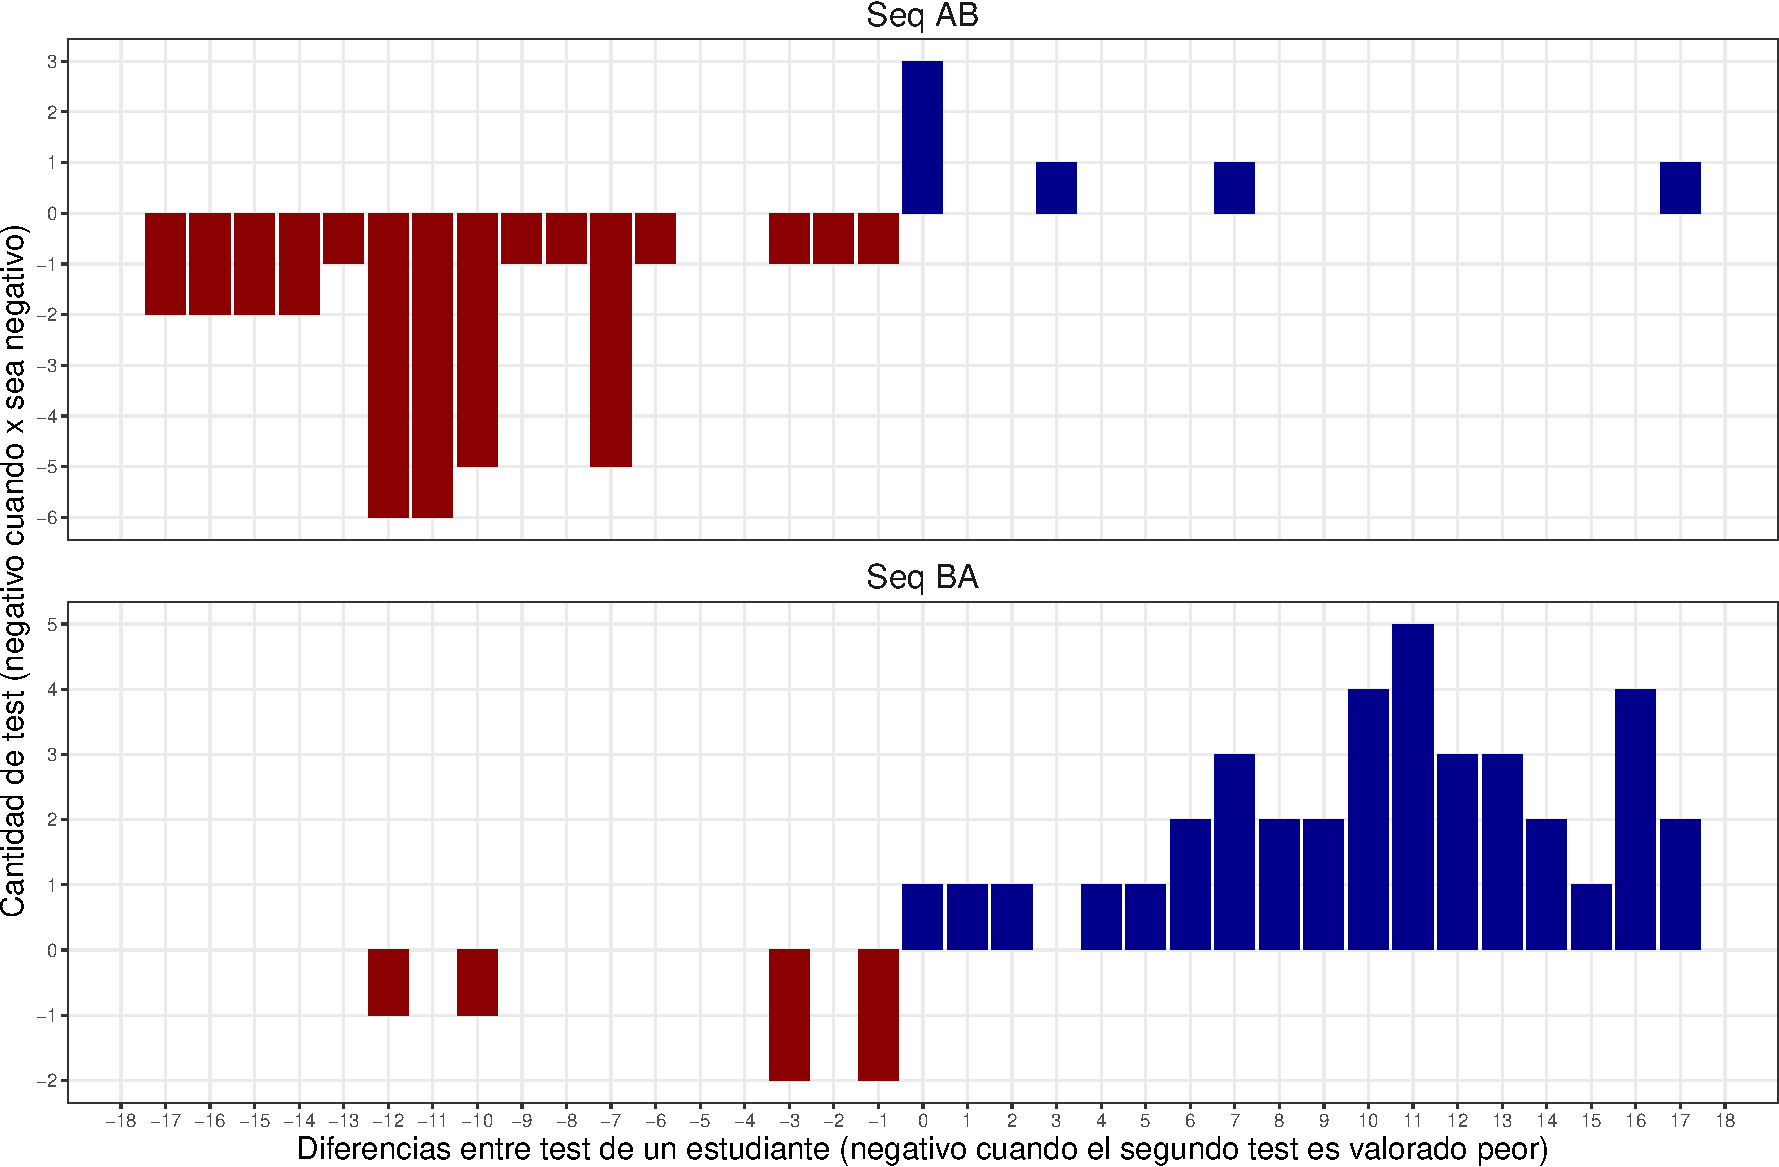
\includegraphics{4_files/figure-pdf/fig-diff-1.pdf}

}

\caption{\label{fig-diff}Frecuencias absolutas de las diferencias en las
respuestas entre test por estudiante y grupo.}

\end{figure}

Vemos que en el grupo \(AB\) las diferencias tienden a ser negativas y
en el \(BA\) positivas. Esto estaría indicando que los estudiantes
valoran mejor el subtitulado de nivel \(A\) en ambas secuencias. Por
ello es esperable que las respuestas de los estudiantes del grupo \(AB\)
hayan empeorado y que las diferencias sean negativas y que lo contrario
haya sucedido con las del grupo \(BA\). La diferencia más frecuente en
el grupo \(AB\) es 12 y en el grupo \(BA\) este valor es 11. f Resulta
llamativo que haya estudiantes cuyas contestaciones estén tan alejadas
de la tendencia de su grupo. En la Tabla~\ref{tbl-diff} se muestran los
tiempos que han transcurrido entre la realización de los test de
aquellos estudiantes cuyas respuestas difieren de forma importante de su
grupo. Son aquellos que aparecen en azul en la secuencia \(AB\) y en
rojo en la secuencia \(BA\). Se observa que casi todos son tiempos entre
actividades muy cortos. En cualquier caso y, como no son muchos, se ha
decidido no eliminarlos y realizar el análisis con ellos.

\hypertarget{tbl-diff}{}
\begin{longtable}{lrc}
\caption{\label{tbl-diff}Estudiantes que tienen diferencias en sus respuestas muy alejadas de la
tendencia de su grupo. }\tabularnewline

\toprule
Seq & Diff & Minutes \\ 
\midrule
AB & 17 & 1.3 \\ 
AB & 7 & 3.33 \\ 
BA & -10 & 50345.95 \\ 
BA & -12 & 1.7 \\ 
\bottomrule
\end{longtable}

En la Figura~\ref{fig-freqs} se muestra la frecuencia relativa del valor
de respuesta para cada grupo y test en todas la preguntas \footnote{En
  el Tabla~\ref{tbl-resume} se presenta la misma información con los
  valores absolutos.}. Esta es otra forma de comparar los niveles de
subtitulado.

\hypertarget{tbl-resume}{}
\begin{longtable}{cccrrrrrr}
\caption{\label{tbl-resume}Resumen de frecuencias de respuesta. }\tabularnewline

\toprule
 &  &  &  & \multicolumn{5}{c}{Response} \\ 
\cmidrule(lr){5-9}
Seq & Period & Treat & 0 & 1 & 2 & 3 & 4 & 5 \\ 
\midrule
AB & 1 & A & 39 & 2 & 25 & 71 & 203 & 434 \\ 
AB & 2 & B & 43 & 87 & 185 & 121 & 172 & 166 \\ 
BA & 1 & B & 40 & 76 & 174 & 127 & 237 & 138 \\ 
BA & 2 & A & 30 & 2 & 30 & 64 & 345 & 321 \\ 
\bottomrule
\end{longtable}

La Figura~\ref{fig-freqs} muestra algunas cuestiones interesantes:

\begin{itemize}
\item
  El tratamiento (subtitulado) con nivel \(A\) presenta claramente
  mayores valores de respuesta que el \(B\) como ya habíamos visto (ver
  Figura~\ref{fig-diff}).
\item
  En general los dos grupos muestran bastante acuerdo en el subtitulado
  en ambos niveles: En el nivel de tratamiento \(A\) los dos grupos
  tienen una frecuencia relativa similar de respuestas positivas
  (valores 4 y 5). El grupo \(AB\) tiene un 82\% de respuestas positivas
  frente a un 84\% el grupo \(BA\). No obstante, el grupo \(AB\) tiene
  más respuestas con valor 5 que el grupo \(BA\) (56\% frente a 41\%).
  La valoración es también similar entre grupos en el nivel de
  tratamiento \(B\): el grupo \(AB\) tiene 44\% de respuestas positivas
  y 47\% el grupo \(BA\). Las valoraciones negativas (1, 2), la neutra
  (3) y la \enquote*{No sé / No contesto} (0) son también muy similares.
\end{itemize}

\begin{figure}[h]

{\centering 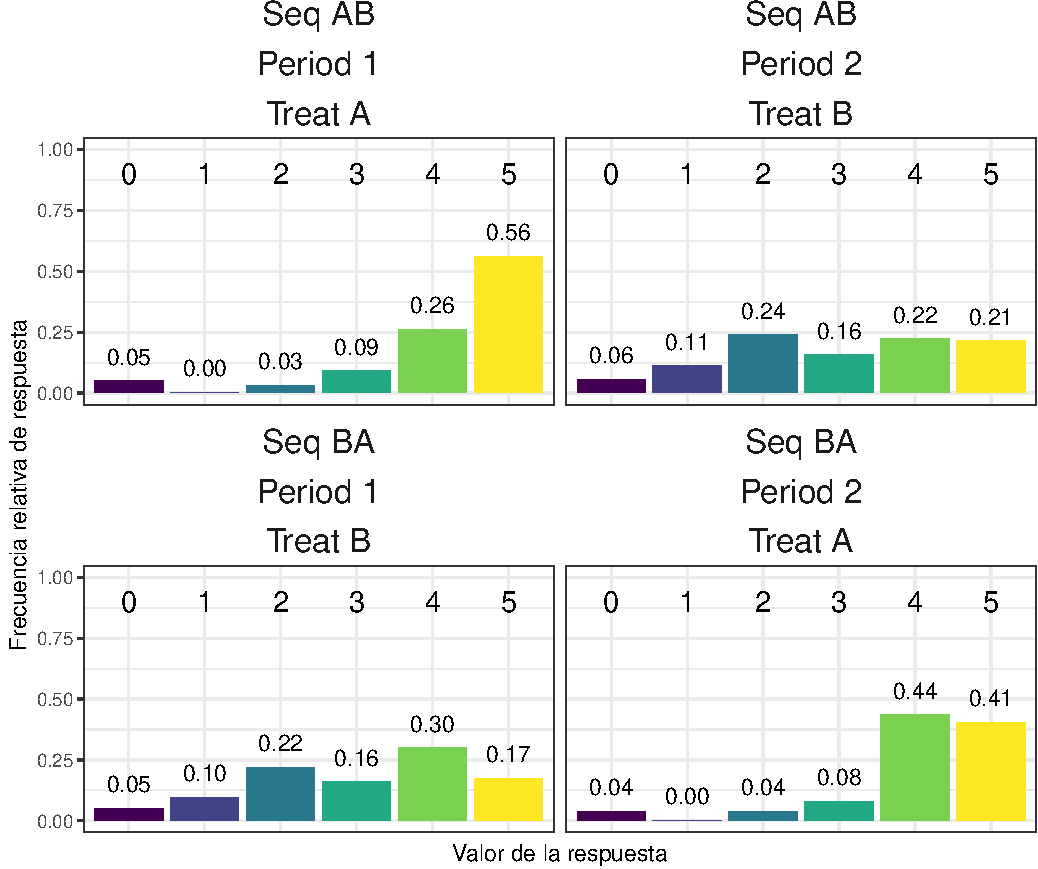
\includegraphics{4_files/figure-pdf/fig-freqs-1.pdf}

}

\caption{\label{fig-freqs}Frecuencias relativas de las respuestas al
test.}

\end{figure}

El análisis marginalizado de tratamiento, secuencia y periodo tiene
estos resultados referidos a las preguntas con contestación positiva (4,
5):

\begin{itemize}
\item
  El tratamiento \(A\) tiene un 83\% marginalizado de respuestas
  positivas frente al 46\% del tratamiento \(B\).
\item
  El periodo 1 tiene un 65\% marginalizado de respuestas positivas
  frente al 64\% del periodo 2.
\item
  Finalmente, la secuencia \(AB\) tiene un 63\% de respuestas positivas
  frente 66\% de la secuencia \(BA\).
\end{itemize}

\hypertarget{anuxe1lisis-de-las-preguntas.}{%
\subsection{Análisis de las
preguntas.}\label{anuxe1lisis-de-las-preguntas.}}

El gráfico Figura~\ref{fig-levels} muestra la frecuencia relativa por
grupo y por test de las preguntas clasificadas por niveles de respuesta,
considerando que:

\begin{itemize}
\tightlist
\item
  Los niveles 1 y 2 se consideran valoraciones negativas.
\item
  El nivel 3 se considera neutro.
\item
  Los niveles 4 y 5 se consideran positivos.
\item
  El nivel 0 (\enquote{No sé / No contesto}) se excluye en este
  análisis.
\end{itemize}

Se muestra en primer lugar la pregunta 18 por ser una valoración global
del subtitulado y que resume la opinión que sobre el mismo tiene el
estudiante. Volvemos a constatar que el subtitulado \(A\) es mejor
valorado por los estudiantes, pero ahora vemos que en las 18 preguntas
ambos grupos tienen más puntuaciones positivas y menos negativas en el
subtitulado \(A\) que el \(B\). También volvemos a encontrar que los dos
grupos valoran de forma muy similar los dos niveles de subtitulado en
todas las preguntas. En el nivel de subtitulado \(A\) las preguntas
\(Q15\), \(Q16\) y \(Q17\) obtienen relativamente peores valoraciones
(consultar la Tabla~\ref{tbl-likert-scale} para ver el texto de las
preguntas) y estas son similares en ambos subtitulados. Hay algunas
preguntas que son valoradas de forma positiva incluso en el nivel de
subtitulado \(B\) (por ejemplo \(Q04\) o \(Q13\)) y que, por lo tanto,
su valoración es similar en ambos subtitulados. Por último, las
preguntas \(Q05\) y \(Q09\) (también la \(Q14\) pero solo para el grupo
\(BA\)) tienen una valoración muy negativa en el nivel de subtitulado
\(B\).

\begin{figure}[h]

{\centering 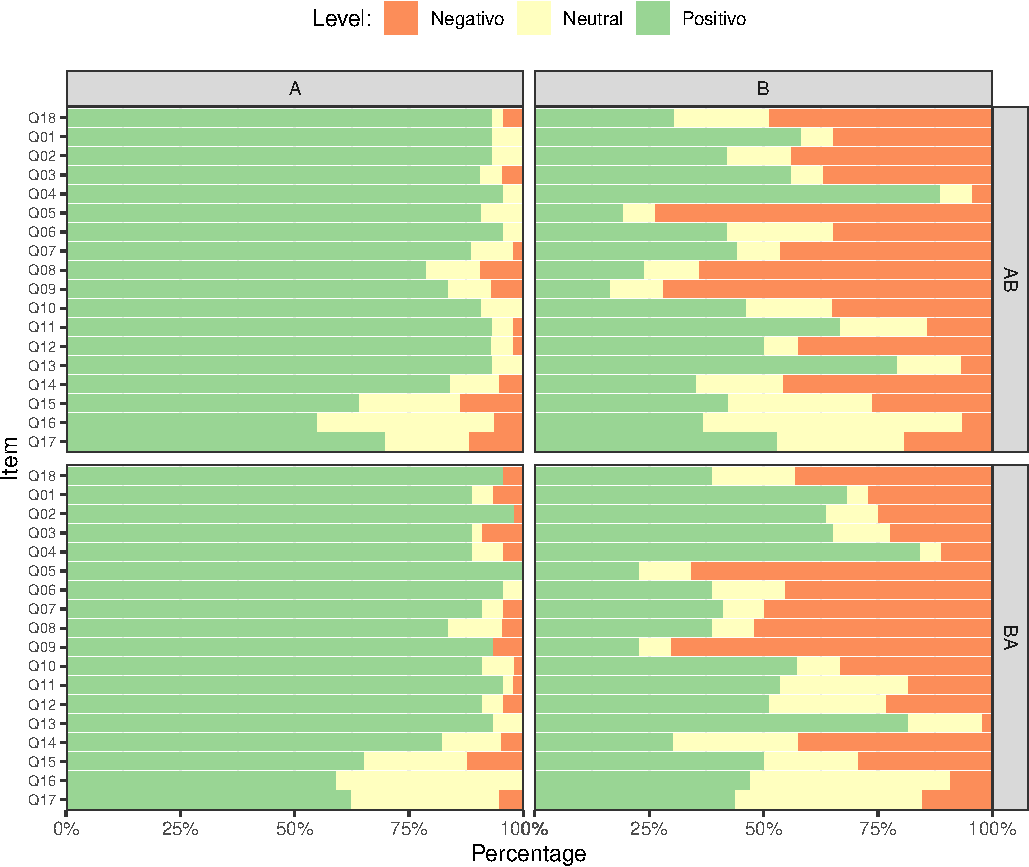
\includegraphics{4_files/figure-pdf/fig-levels-1.pdf}

}

\caption{\label{fig-levels}Frecuencias relativas de las respuestas por
pregunta.}

\end{figure}

La figura Figura~\ref{fig-likert} clasifica las preguntas por valoración
y permite constatar lo que ya habíamos visto en el párrafo anterior con
mayor comodidad.

\begin{figure}

\begin{minipage}[t]{0.50\linewidth}

{\centering 

\raisebox{-\height}{

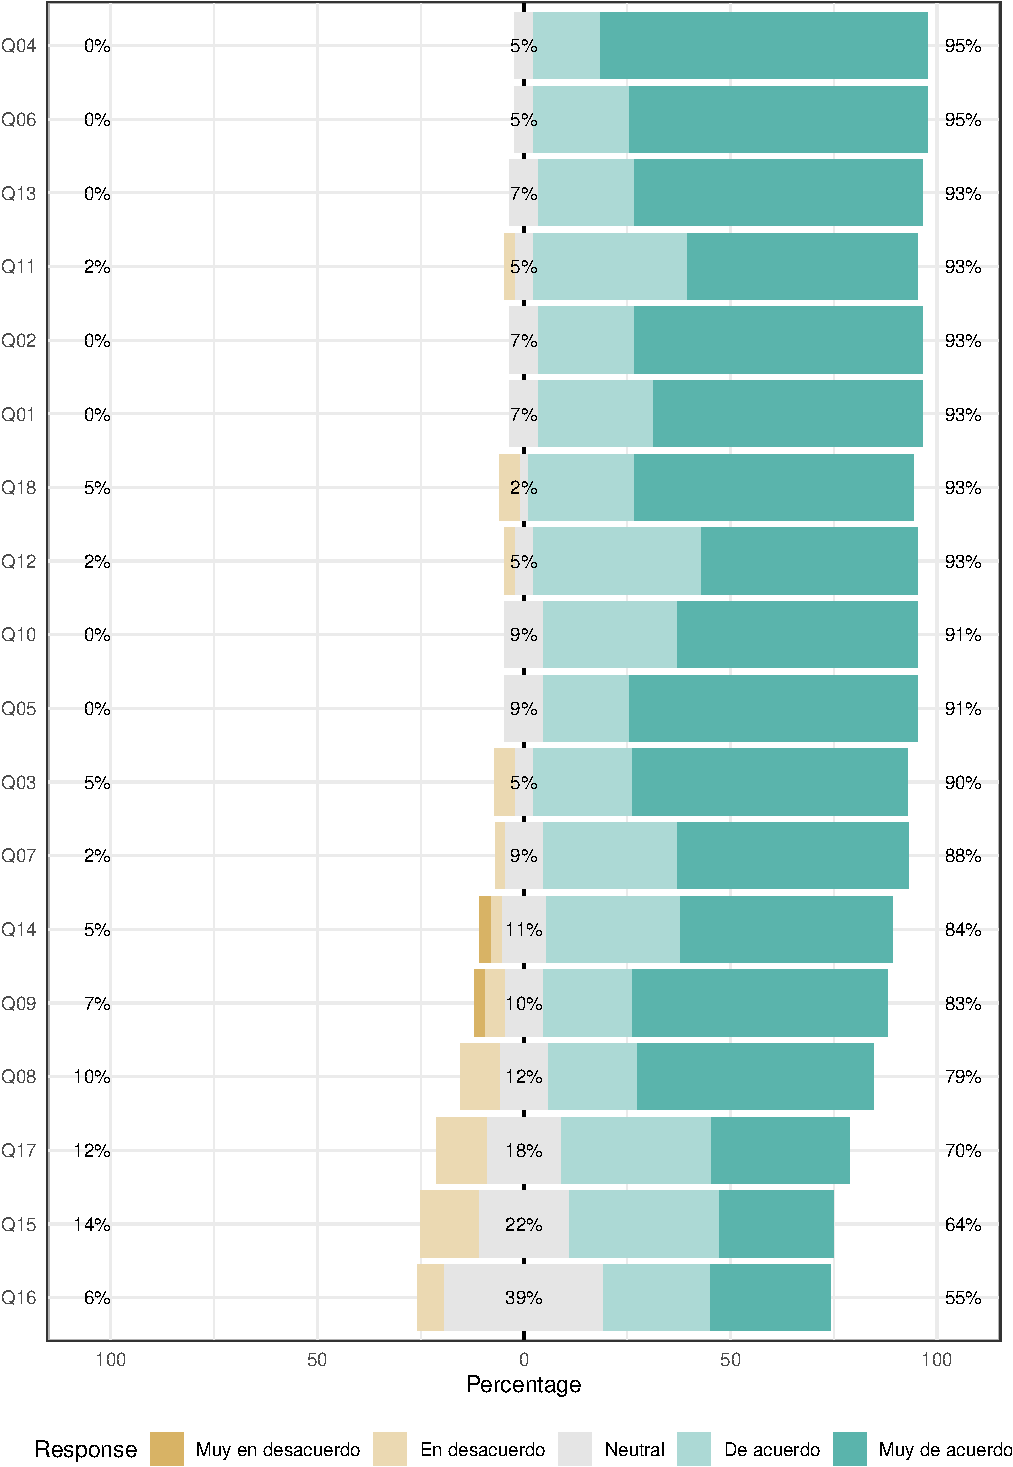
\includegraphics{4_files/figure-pdf/fig-likert-1.pdf}

}

}

\subcaption{\label{fig-likert-1}Seq AB , Treat A}
\end{minipage}%
%
\begin{minipage}[t]{0.50\linewidth}

{\centering 

\raisebox{-\height}{

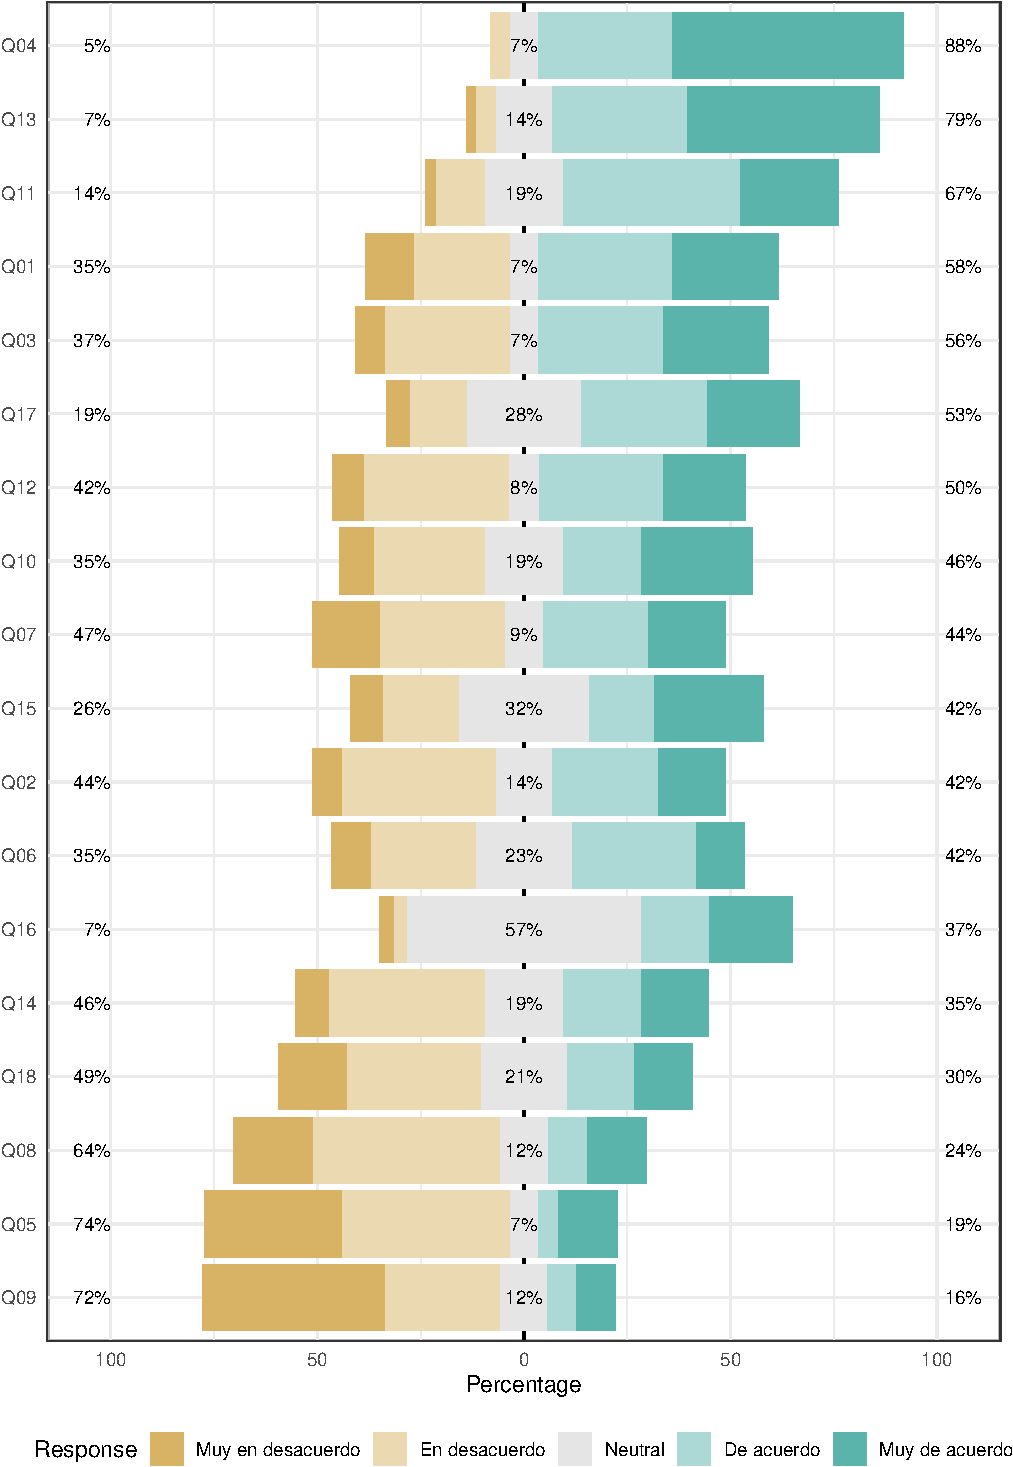
\includegraphics{4_files/figure-pdf/fig-likert-2.pdf}

}

}

\subcaption{\label{fig-likert-2}Seq AB , Treat B}
\end{minipage}%
\newline
\begin{minipage}[t]{0.50\linewidth}

{\centering 

\raisebox{-\height}{

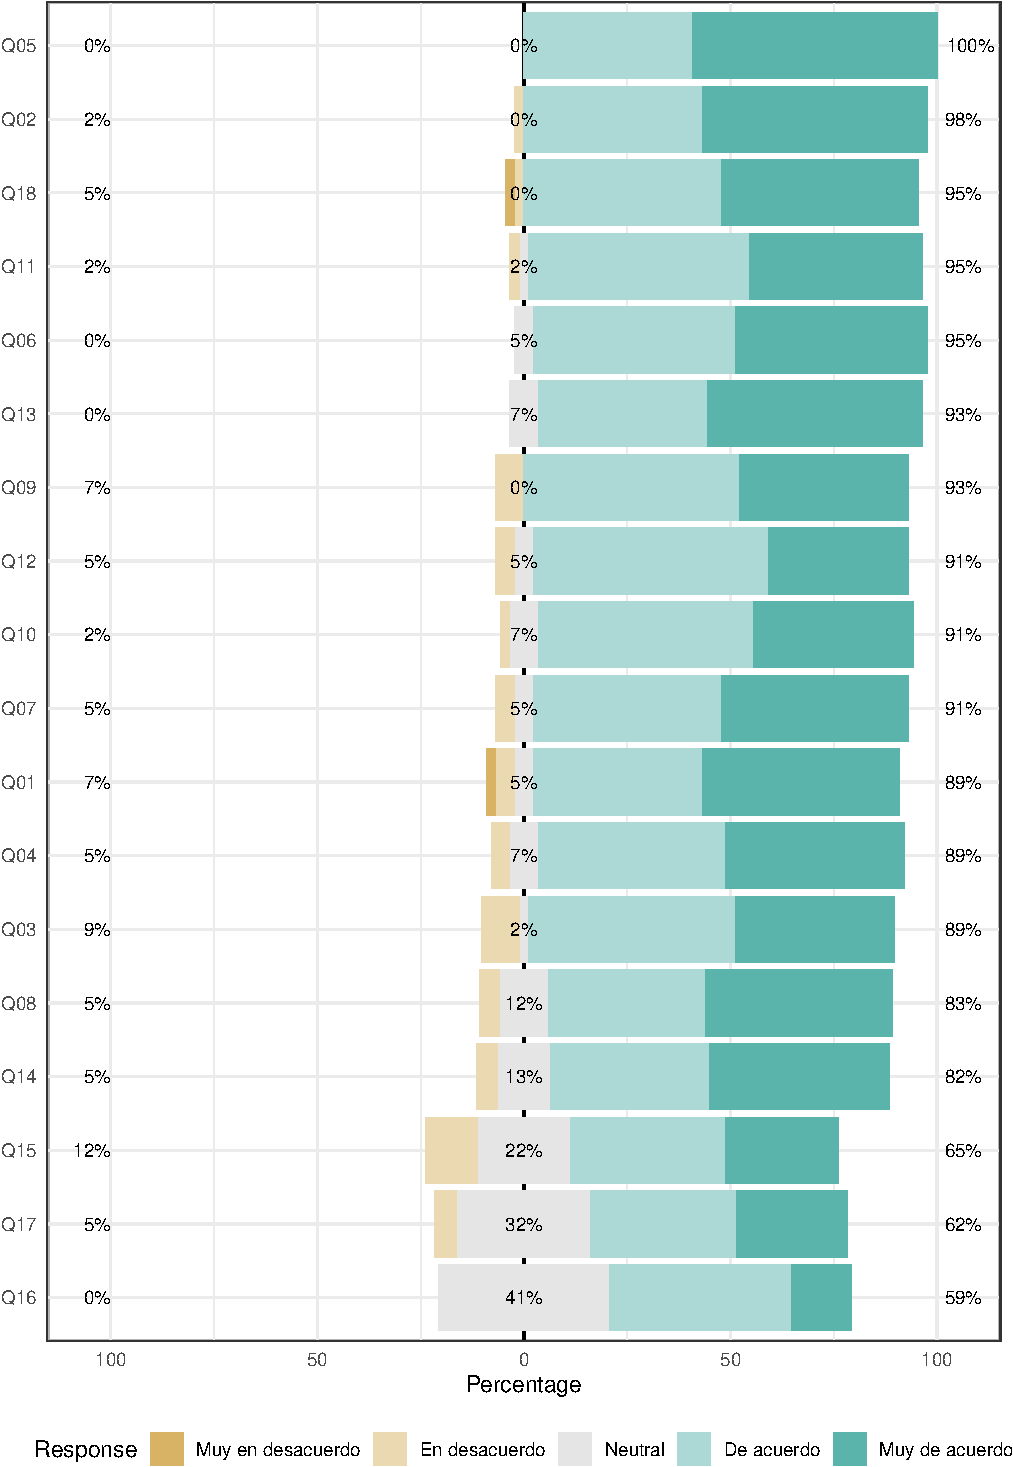
\includegraphics{4_files/figure-pdf/fig-likert-3.pdf}

}

}

\subcaption{\label{fig-likert-3}Seq BA , Treat A}
\end{minipage}%
%
\begin{minipage}[t]{0.50\linewidth}

{\centering 

\raisebox{-\height}{

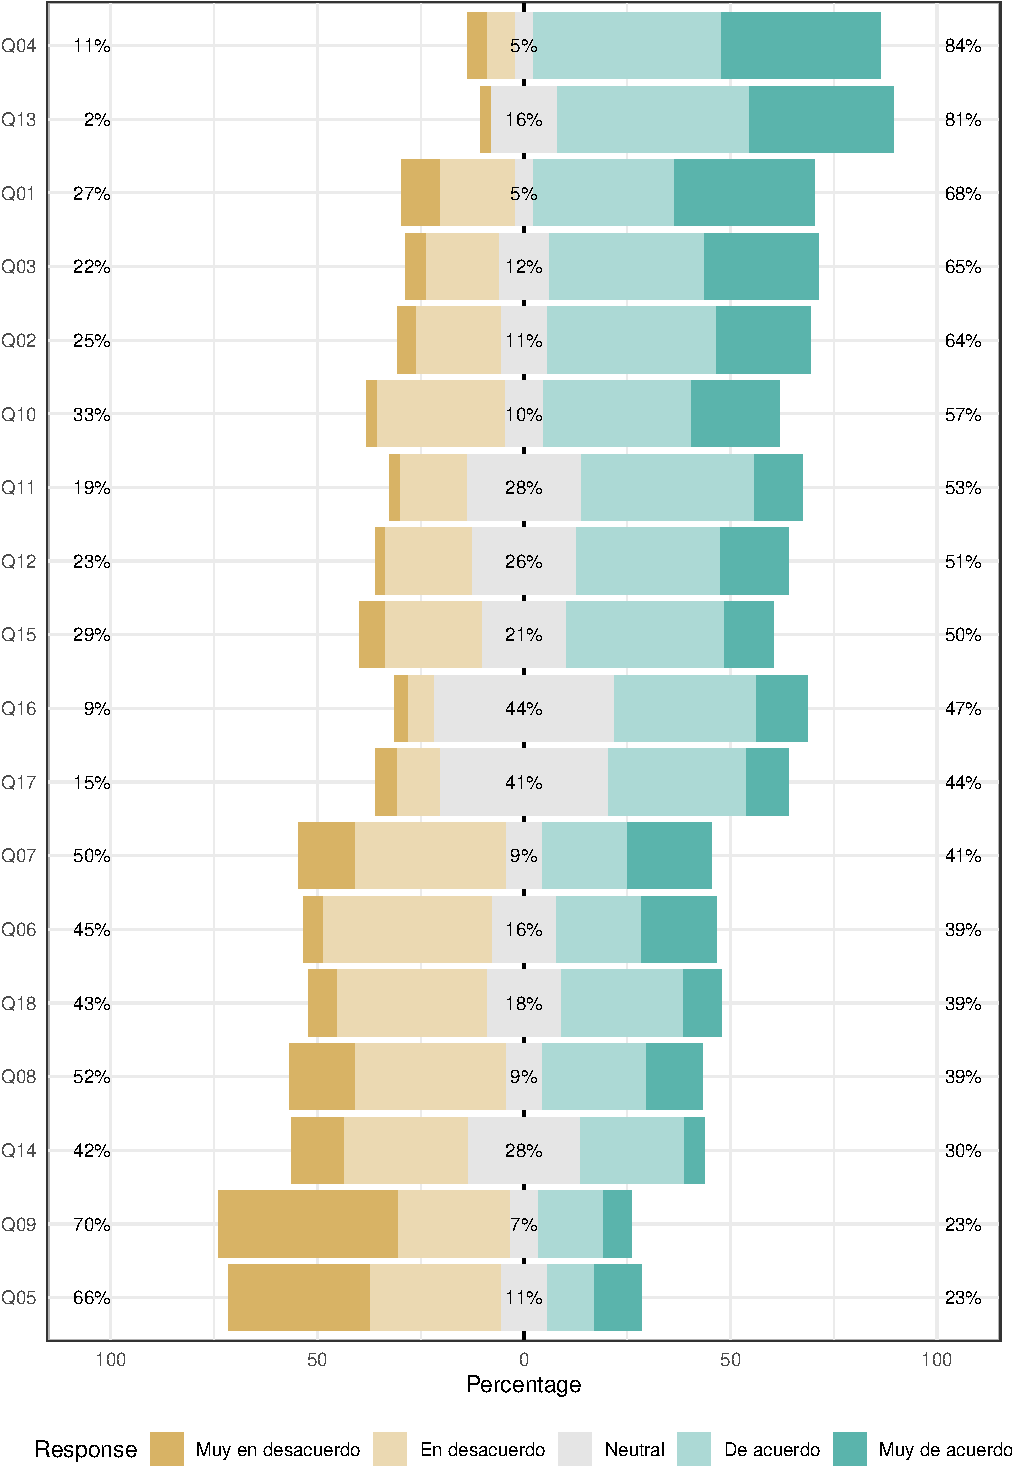
\includegraphics{4_files/figure-pdf/fig-likert-4.pdf}

}

}

\subcaption{\label{fig-likert-4}Seq BA , Treat B}
\end{minipage}%

\caption{\label{fig-likert}Preguntas ordenadas por valoración.}

\end{figure}

En la Figura~\ref{fig-improve} se muestra para cada pregunta la
proporción de estudiantes que han valorado mejor el subtitulado \(A\)
que el \(B\) \footnote{Se han eliminado las preguntas en las que una de
  las dos respuestas del usuario ha sido \enquote{No sé / No contesto}.
  La comparación realizada es respuesta en \(A > B\) frente a
  \(A <= B\).}. Se comprueba que la mayoría de las preguntas superan el
50\%, lo que indica que los estudiantes valoran mejor el subtitulado
\(A\).

\begin{figure}[h]

{\centering 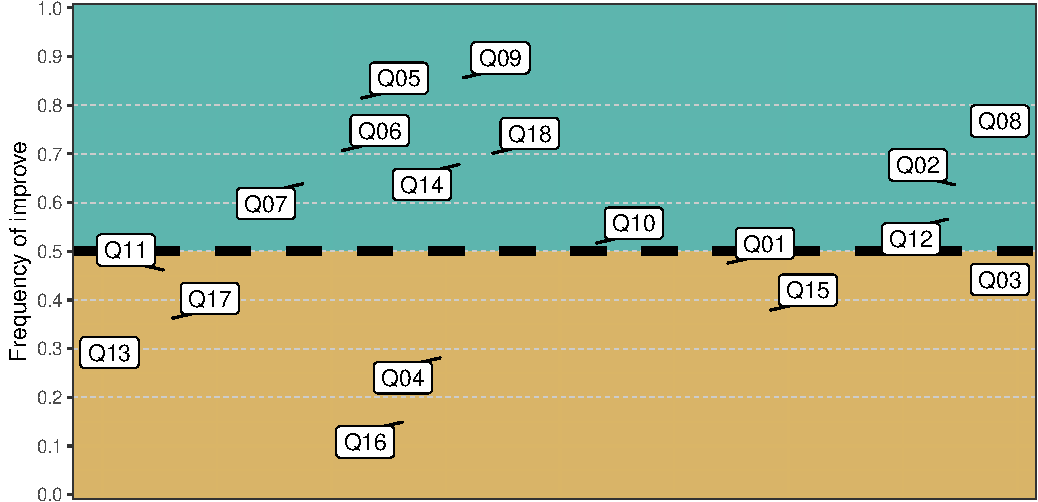
\includegraphics{4_files/figure-pdf/fig-improve-1.pdf}

}

\caption{\label{fig-improve}Frecuencia de preguntas que mejoran por
estudiante entre subtitulados (A \textgreater{} B)}

\end{figure}

\begin{figure}[h]

{\centering 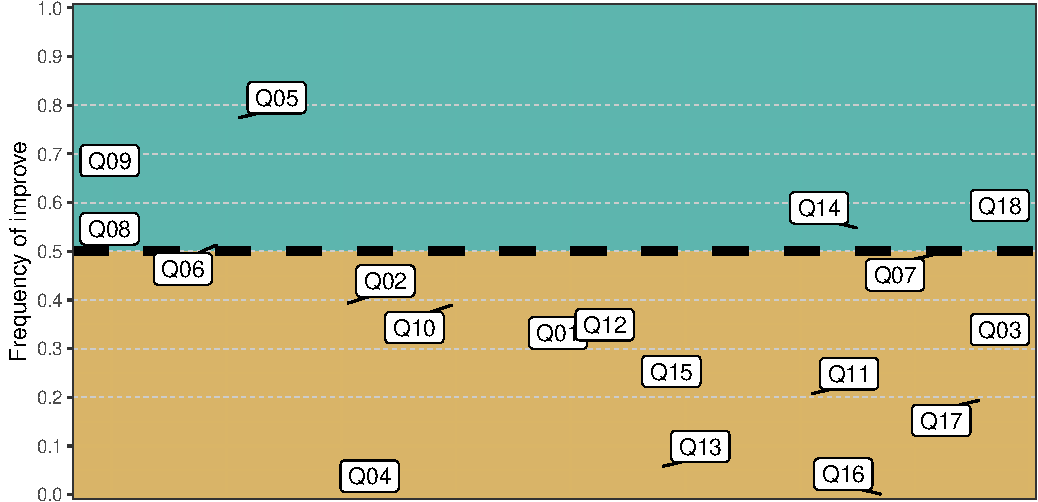
\includegraphics{4_files/figure-pdf/fig-improve-2-1.pdf}

}

\caption{\label{fig-improve-2}Frecuencia de preguntas que mejoran por
estudiante entre subtitulados (positive A vs negative B)}

\end{figure}

En la Figura~\ref{fig-improve-2} se hace una comparación más exigente ya
que ahora se muestra la frecuencia con la que los estudiantes cambian el
nivel del subtitulado: de haber valorado el subtitulado positivamente (4
ó 5) en \(A\) a hacerlo de forma negativa en \(B\) (1 ó 2). En esta
ocasión solo las preguntas Q18, Q05, Q06, Q08, Q09, Q14 superan el 50\%.

\hypertarget{sec-modelos-utilizados}{%
\section{Modelos utilizados}\label{sec-modelos-utilizados}}

Algunas de las técnicas de análisis y modelado estadístico propuesto en
la Sección~\ref{sec-modelos-utilizados} requieren concreción y
adaptación para poder ser utilizadas en el diseño de experimento de
subtitulado. En esta sección se explica la forma concreta de aplicarlas
y los paquetes y configuración en R utilizados. También se justifican
las variables incluidas en cada modelo. La presentación de los
resultados se pospone al Capítulo~\ref{sec-resultados}.

\hypertarget{sec-or-2}{%
\subsection{\texorpdfstring{Comparación con \emph{Odds
Ratio}}{Comparación con Odds Ratio}}\label{sec-or-2}}

En la sección Sección~\ref{sec-or} se explicó el fundamento teórico de
esta técnica. Aquí se expone como se puede aplicar al diseño de
experimento que se está analizando. Dado que los factores \(Treat\),
\(Period\) y \(Seq\) tienen todos 2 niveles, podemos contrastar si hay
interacción entre ellos para cada nivel de respuesta. Es decir, se
contrasta la hipótesis \(H_0: OR=1\) de ausencia de interacción frente a
\(H_1: OR \neq 1\) de existencia de interacción en algún nivel de
respuesta. Por ejemplo, el \(OR\) para el nivel respuesta \(r\) entre
subtítulos y secuencias se define de la siguiente forma:

\[
OR_{(Treat, Seq \mid Response=r)}=\frac{
    \frac{
            P(Treat=A \mid Seq=AB, Response=r)
        }{
            P(Treat=B \mid Seq=AB, Response=r)
        }
    }
    {\frac{
        P(Treat=A \mid Seq=BA, Response=r)
        }{
        P(Treat=B \mid Seq=BA, Response=r)
    }
}
\]

Si los \(odds\) son similares en cada nivel de respuesta, podemos
aceptar que la hipótesis nula de que los grupos responden de forma
similar a cada nivel de subtitulado. Se hará un test similar pero entre
subtitulado y periodos. Para realizar el contraste de hipótesis se
utilizará la función \(loddsratio\) del paquete \(vcd\).

\hypertarget{sec-logistica-2}{%
\subsection{Regresión Logística}\label{sec-logistica-2}}

En la Sección~\ref{sec-logistica} se presentó el fundamento teórico de
la Regresión Logística. En esta sección se justifica el uso de este
modelo y se ajustan y comparan varios modelos. La variable respuesta se
compone de 5 valores ordenados. Esto imposibilita usar directamente la
Regresión Logística ya que requiere que la variable de respuesta sea
dicotómica. No obstante, se puede comparar la respuesta que cada
estudiante dio a cada uno de los subtitulados y comprobar si ha
mejorado. Esto producirá una variable de respuesta binaria que permitirá
el uso de la Regresión Logística. No obstante, esta transformación
reducirá la cantidad de datos disponibles a la mitad e impedirá analizar
el efecto periodo ya que al comparar los subtitulados, desaparece el
periodo. Se ha transformado el \texttt{dataframe} de tal forma que si un
usuario valoró una pregunta mejor en el subtitulado \(A\) que en el
\(B\), se consigna 1 en la variable respuesta, si empeoró o puntuó igual
se consigna 0. Si en uno de los test valora una pregunta con \enquote{No
sé / No contesto}, se elimina esa pregunta.

Se ajusta el modelo con la secuencia como predictor. Se constata que el
coeficiente del intercepto es positivo y significativo. El intercepto es
el \(log\ odds\) de mejorar la valoración en \(A\) sobre \(B\) respecto
a empeorar la valoración. Sin embargo, la secuencia no resulta
significativa y además añadirla apenas reduce la \enquote{deviance}, por
lo que el modelo nulo sin predictores resulta más parsimonioso. Se
podrían añadir como predictores las preguntas y los estudiantes. No se
hace aquí y se pospone la sección de resultados.

\begin{verbatim}

Call:
glm(formula = Improve ~ 1 + Seq, family = "binomial", data = df_improve)

Coefficients:
            Estimate Std. Error z value Pr(>|z|)    
(Intercept)  0.36572    0.08563   4.271 1.94e-05 ***
SeqBA       -0.18153    0.11913  -1.524    0.128    
---
Signif. codes:  0 '***' 0.001 '**' 0.01 '*' 0.05 '.' 0.1 ' ' 1

(Dispersion parameter for binomial family taken to be 1)

    Null deviance: 1575.8  on 1151  degrees of freedom
Residual deviance: 1573.5  on 1150  degrees of freedom
AIC: 1577.5

Number of Fisher Scoring iterations: 4
\end{verbatim}

\hypertarget{sec-ordinal-2}{%
\subsection{Regresión Ordinal}\label{sec-ordinal-2}}

En la Sección~\ref{sec-ordinal} se presentó el fundamento teórico de la
Regresión Ordinal Acumulativa. En esta sección se ajustan algunos
modelos y se interpretan los resultados.

\hypertarget{comprobaciuxf3n-de-los-presupuestos-del-modelo}{%
\subsubsection{Comprobación de los presupuestos del
modelo}\label{comprobaciuxf3n-de-los-presupuestos-del-modelo}}

La Regresión Ordinal presupone que los \(odds\) entre dos niveles de
respuesta son proporcionales para los mismos valores de variables
explicativas. Como se vio en la Ecuación~\ref{eq-ordinal2}, es
equivalente comprobar que los \(odds\) son proporcionales que comprobar
que la diferencia en \texttt{logits} es constante. Una forma de hacer
esto es calcular la diferencia en \texttt{logits} entre dos niveles de
respuesta consecutivos en cada valor de cada variable predictiva y
comparar si las diferencias son similares
\autocite[ver][pp.~315-316]{harrell2015}. En la
Figura~\ref{fig-po.check} se han calculado para los predictores
\texttt{Treat}, \texttt{Period}, \texttt{Seq} y \texttt{Question} las
diferencias de \(odds\) entre cada dos niveles consecutivos de
respuesta. Se constata que las diferencias son pequeñas particularmente
para el periodo y para la secuencia. También son moderadas para la
mayoría de las preguntas. La diferencia es mayor en el subtitulado de en
la comparación de los niveles 1 y 2. Con esta evidencia, se acepta la
hipótesis de proporcionalidad de \(odds\).

\begin{figure}[h]

{\centering 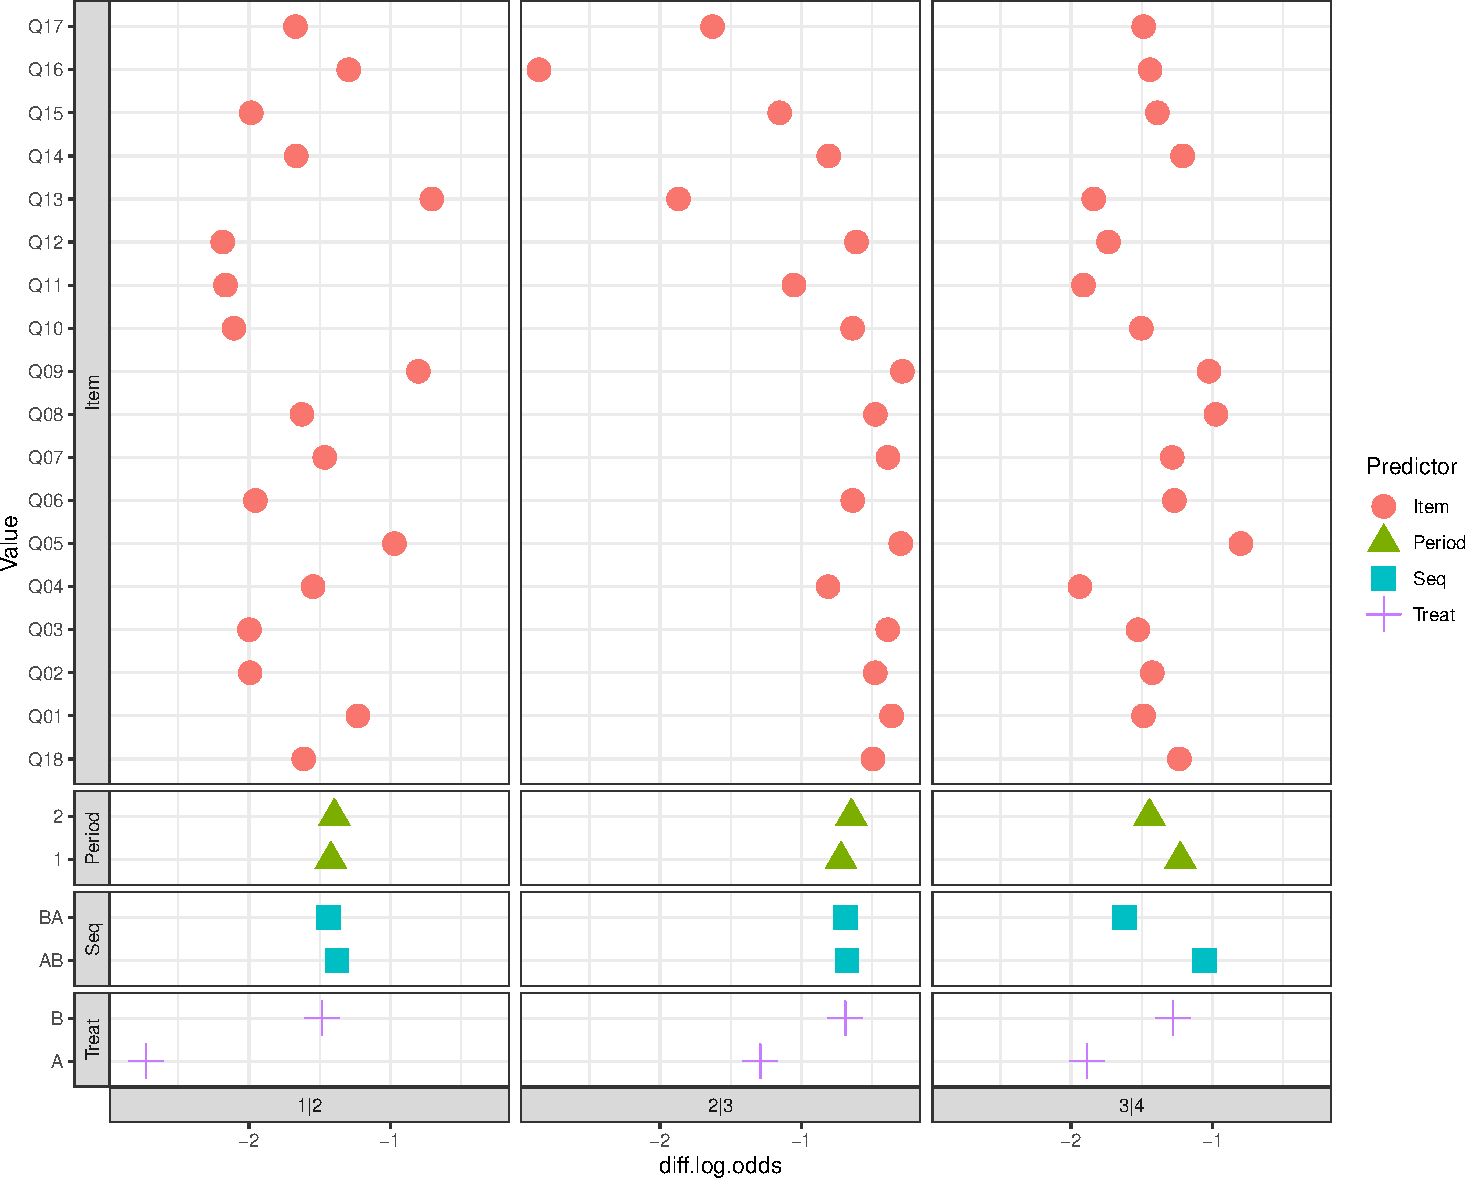
\includegraphics{4_files/figure-pdf/fig-po.check-1.pdf}

}

\caption{\label{fig-po.check}Comprobación de la proporcionalidad de
\emph{odds}.}

\end{figure}

\hypertarget{ajuste-del-modelo-ordinal-response-treat}{%
\subsubsection{\texorpdfstring{Ajuste del modelo ordinal
\texttt{Response\ \textasciitilde{}\ Treat}}{Ajuste del modelo ordinal Response \textasciitilde{} Treat}}\label{ajuste-del-modelo-ordinal-response-treat}}

Existen varios paquetes en R que permiten ajustar una Regresión Ordinal
con función de enlace logística. El más popular es el paquete
\texttt{Ordinal} \autocite{ordinalR}. El paquete \texttt{VGAM}
\autocite{VGAMR} es más flexible y potente. Otra posibilidad es usar la
función \texttt{polr} del paquete \texttt{MASS} \autocite{MASSR}.
Finalmente la función \texttt{orm} del paquete \texttt{rms} también
permite hacerlo \autocite[ver][]{harrell2015}. En este trabajo usaremos
el paquete \texttt{Ordinal} por permitir también incluir efectos
aleatorios que utilizaremos en un apartado posterior. Comenzamos con un
modelo simple que tiene como único predictor el nivel de subtitulado por
ser la variable objetivo de nuestro modelo:

\[
\text{logit}(P(Response_i \leq k)) = \tau_k - \beta_1 \text{Treat}_i,
\]

\scriptsize

\begin{verbatim}
formula: Response ~ 1 + Treat
data:    df_clean

 link  threshold nobs logLik   AIC     niter max.grad cond.H 
 logit flexible  2980 -3966.11 7942.21 5(0)  1.64e-10 3.1e+01

Coefficients:
       Estimate Std. Error z value Pr(>|z|)    
TreatB  -1.7206     0.0731  -23.54   <2e-16 ***
---
Signif. codes:  0 '***' 0.001 '**' 0.01 '*' 0.05 '.' 0.1 ' ' 1

Threshold coefficients:
    Estimate Std. Error z value
1|2 -3.97230    0.09678 -41.045
2|3 -2.45446    0.06812 -36.029
3|4 -1.66453    0.05936 -28.042
4|5 -0.10547    0.04946  -2.132
\end{verbatim}

\normalsize

El método \texttt{summary()} muestra la información resumen. Para su
interpretación vamos a seguir \textcite{christensen2018CumulativeLM}. El
número de condición Hessiano es inferior a \(10^4\) lo que es indicativo
de que no hay problemas de optimización \footnote{El número de condición
  de Hessiano es una medida de la curvatura de una función en un punto.
  Si el número de condición de Hessiano es grande, la función es muy
  sensible a pequeñas perturbaciones y puede ser difícil de optimizar.}.
La sección de coeficientes es la más importante. Se muestra la
estimación de parámetros, el error estándar y la significación
estadística de acuerdo al test de Wald \footnote{El test de Wald es un
  contraste de hipótesis estadístico en el que se evalúa si el valor
  estimado es cero suponiendo que
  \(W = \left(\frac{\hat{\theta} - \theta_0}{se(\hat{\theta})}\right)^2 \sim \chi^{2}\)
  .}. Se comprueba que el valor es claramente significativo. Es decir,
que los estudiantes han valorado de forma diferente la calidad del
subtitulado en ambos vídeos. El estimador de maxima verosimilitud del
coeficiente \texttt{TreatB} es -1.72. Siguiendo la deducción de
\textcite{bruin2011} podemos, por ejemplo, hacer la siguiente
interpretación del significado de este coeficiente referido a dos
niveles consecutivos de respuesta:

\[
\begin{aligned}
logit [P(Y \le 1)] & = & -3.97 - (-1.72 x_1) \\
logit [P(Y \le 2)] & = & -2.45 - (-1.72 x_1)
\end{aligned}
\]

Por lo tanto y teniendo en cuenta que \(x_1 = 1\) cuando \(Treat = B\) y
\(x_1 = 0\) cuando \(Treat = A\), se pueden calcular los \(odds\) de
\(A\) y de \(B\):

\[
\begin{aligned}
\frac{P(Y \le 1 \mid x_1 = B)}{P(Y > 1 \mid x_1 = B)} & = & exp(-3.97)/exp(-1.72) \\
\frac{P(Y \le 1 \mid x_1 = A)}{P(Y > 1 \mid x_1 = A)} & = & exp(-3.97) \\
\frac{P(Y \le 2 \mid x_1 = B)}{P(Y > 2 \mid x_1 = B)} & = & exp(-2.45)/exp(-1.72) \\
\frac{P(Y \le 2 \mid x_1 = A)}{P(Y > 2 \mid x_1 = A)} & = & exp(-2.45)
\end{aligned}
\]

Y los \(OR\):

\[
\begin{aligned}
\frac{P(Y \le 1 | x_1=B)}{P(Y > 1 | x_1=B)} / \frac{P(Y \le 1 | x_1=A)}{P(Y > 1 | x_1=A)} & = & 1/exp(-1.72) & = & 5.59 \\
\frac{P(Y \le 2 | x_1=B)}{P(Y > 2 | x_1=B)} / \frac{P(Y \le 2 | x_1=A)}{P(Y > 2 | x_1=A)} & = & 1/exp(-1.72) & = & 5.59 \\
\end{aligned}
\]

Se comprueba que el \(OR\) es equivalente en todos los niveles de
respuesta al cuestionario. Esta es una de las suposiciones de la
regresión ordinal acumulativa. El \(odds\) de respuesta al cuestionario
entre los niveles inferiores y superiores a uno dado, \(k\), es 5.59
veces en el subtitulado \(B\) que en el \(A\). Esto indica que el
subtitulado \(B\) es percibido por los estudiantes como de peor calidad
que el subtitulado \(A\). Concretamente, el coeficiente \(\beta\) para
\texttt{Treat} es el \texttt{log\ OR} de observar una mejor respuesta en
una pregunta del test es 5.59 veces superior en el nivel de subtitulado
\(A\) que en el \(B\). Aunque no suele ser de interés la interpretación
de los coeficientes de los umbrales (\texttt{Threshold\ coefficients}),
se pueden utilizar para estimar las probabilidades de respuesta. Por
ejemplo, para el nivel de subtitulado \(B\) y nivel de respuesta 2:

\[
\begin{aligned}
logit [P(Y \le 1)] & = & -3.97 - (-1.72) & = & -2.25 \\
P(Y \le 1) & = & \frac{exp(-2.25)}{1 + exp(-2.25)} & = & 0.10 \\
logit [P(Y \le 2)] & = & -2.45 - (-1.72) & = & -0.73 \\
P(Y \le 2) & = & \frac{exp(-0.73)}{1 + exp(-0.73)} & = & 0.32 \\
P(Y = 2) & = & P(Y \le 2) - P(Y \le 1) & = &  0.23 
\end{aligned}
\]

Para el subtitulado \(A\) no se tiene en cuenta el coeficiente
\(TreatB\) ya que el valor \(x_1\) es cero:

\[
\begin{aligned}
logit [P(Y \le 1)] & = & & & -3.97 \\
P(Y \le 1) & = & \frac{exp(-3.97)}{1 + exp(-3.97)} & = & 0.02 \\
logit [P(Y \le 2)] & = & & & -2.45 \\
P(Y \le 2) & = & \frac{exp(-2.45)}{1 + exp(-2.45)} & = & 0.08 \\
P(Y = 2) & = & P(Y \le 2) - P(Y \le 1) & = &  0.06 
\end{aligned}
\]

En Tabla~\ref{tbl-probs-clm-treat} se muestran las probabilidades para
ambos niveles de subtitulado y todos los posibles valores de respuesta.

\hypertarget{tbl-probs-clm-treat}{}
\begin{table}
\caption{\label{tbl-probs-clm-treat}Probabilidades de respuesta para el modelo ordinal Response
\textasciitilde{} Treat }\tabularnewline

\centering
\begin{tabular}{l|r|r|r|r|r}
\hline
  & 1 & 2 & 3 & 4 & 5\\
\hline
A & 0.018 & 0.061 & 0.08 & 0.315 & 0.526\\
\hline
B & 0.095 & 0.229 & 0.19 & 0.320 & 0.166\\
\hline
\end{tabular}
\end{table}

\hypertarget{sec-response-treat.period}{%
\subsubsection{\texorpdfstring{Ajuste del modelo ordinal
\texttt{Response\ \textasciitilde{}\ Treat\ *\ Period}}{Ajuste del modelo ordinal Response \textasciitilde{} Treat * Period}}\label{sec-response-treat.period}}

Para saber si existe un efecto periodo, añadimos como predictor la
variable \texttt{Period}. También se añade la interacción entre
subtitulado y periodo:

\small

\begin{equation}\protect\hypertarget{eq-ordinal-3}{}{
\text{logit}(P(Response_i \leq k)) = \tau_k - \beta_1 \text{Treat}_i - \beta_2 \text{Period}_i - \beta_3 \text{Treat}_i * \text{Period}_i
}\label{eq-ordinal-3}\end{equation}

\normalsize

En el Apéndice~\ref{sec-contrasts} se demuestra que cuando el contraste
es \(sum\) la interacción entre periodo y subtitulado es equivalente al
efecto secuencia. Es decir, que los modelos
\texttt{Response\ \textasciitilde{}\ Treat*Period} y
\texttt{Response\ \textasciitilde{}\ Treat\ +\ Period\ +\ Seq} son
equivalentes. Esto no sucede cuando el contraste es \(treatment\), que
es el utilizado por defecto en R. En la Tabla~\ref{tbl-contrast} se
comparan los coeficientes de los cuatro modelos que se listan a
continuación:

\begin{itemize}
\tightlist
\item
  \texttt{Response\ \textasciitilde{}\ Treat\ *\ Period} con contraste
  \texttt{treatment}.
\item
  \texttt{Response\ \textasciitilde{}\ Treat\ +\ Period\ +\ Seq} con
  contraste \texttt{treatment}.
\item
  \texttt{Response\ \textasciitilde{}\ Treat\ *\ Period} con contraste
  \texttt{sum}.
\item
  \texttt{Response\ \textasciitilde{}\ Treat\ +\ Period\ +\ Seq} con
  contraste \texttt{sum}.
\end{itemize}

\tiny

\hypertarget{tbl-contrast}{}
\begin{longtable}{lrlrlrlr}
\caption{\label{tbl-contrast}Comparación de los coeficientes con contraste ``treatment'' y ``sum''. }\tabularnewline

\toprule
\multicolumn{4}{c}{contr.treatment} & \multicolumn{4}{c}{contr.sum} \\ 
\cmidrule(lr){1-4} \cmidrule(lr){5-8}
\multicolumn{2}{c}{Response \textasciitilde{} Treat*Period} & \multicolumn{2}{c}{Response \textasciitilde{} Treat+Period+Seq} & \multicolumn{2}{c}{Response \textasciitilde{} Treat*Period} & \multicolumn{2}{c}{Response \textasciitilde{} Treat+Period+Seq} \\ 
\cmidrule(lr){1-2} \cmidrule(lr){3-4} \cmidrule(lr){5-6} \cmidrule(lr){7-8}
coef & value & coef & value & coef & value & coef & value \\ 
\midrule
1|2 & $-4.246$ & 1|2 & $-4.246$ & 1|2 & $-3.127$ & 1|2 & $-3.127$ \\ 
2|3 & $-2.728$ & 2|3 & $-2.728$ & 2|3 & $-1.608$ & 2|3 & $-1.608$ \\ 
3|4 & $-1.938$ & 3|4 & $-1.938$ & 3|4 & $-0.818$ & 3|4 & $-0.818$ \\ 
4|5 & $-0.370$ & 4|5 & $-0.370$ & 4|5 & $0.750$ & 4|5 & $0.750$ \\ 
TreatB & $-1.960$ & TreatB & $-1.748$ & Treat1 & $0.874$ & Treat1 & $0.874$ \\ 
Period2 & $-0.492$ & Period2 & $-0.279$ & Period1 & $0.140$ & Period1 & $0.140$ \\ 
TreatB:Period2 & $0.425$ & SeqBA & $-0.213$ & Treat1:Period1 & $0.106$ & Seq1 & $0.106$ \\ 
\bottomrule
\end{longtable}

\normalsize

Comprobamos que coinciden los coeficientes de los dos modelos con
contraste \texttt{sum} y que el efecto secuencia es equivalente a la
interacción de periodo y subtitulado con este contraste. Sin embargo, en
el contraste \texttt{treatment} coinciden los coeficientes de los
interceptores pero no así los de los factores. Además, estos tres
últimos coeficientes tienen nombres diferentes en los dos contrastes. La
diferencia en el nombre se corresponde con la diferente interpretación
del significado de los coeficientes. En el contraste \texttt{treatment}
los valores de los interceptos se refieren a los valores de los factores
en el nivel de referencia de cada factor (en este caso \(Treat = A\) y
\(Period = 1\)) y los valores de los otros coeficientes (\(TreatB\) y
\(Period2\)) son la diferencia con el de referencia. Así, por ejemplo,
\(TreatB\) es la diferencia con \(TreatA\) en el periodo 1. Con este
tipo de contraste es más difícil aislar el efecto que produce un nivel
de un factor independiente del otro factor. En el contraste \texttt{sum}
los valores de los interceptos son el efecto medio y los coeficientes
\(Treat1\) y \(Period1\) son los efectos que sobre ese valor medio
produce el nivel de factor de referencia, que en este caso es el primero
(\(Treat = A\) y \(Period = 1\) respectivamente). Así por ejemplo en el
contraste \texttt{sum}:

\begin{itemize}
\tightlist
\item
  El coeficiente \(1|2\) tiene un valor -3.127 y es el \texttt{logit}
  medio de que la respuesta sea menor que 1 frente a que sea mayor que
  1.
\item
  El coeficiente \(Treat1\) tiene un valor de 0.874 y es la diferencia
  en \texttt{logits} que se añade en el nivel de subtitulado \(A\) sin
  tener en cuenta el periodo. Es decir, que es el efecto del subtitulado
  \(A\). Su valor es positivo, como en la Ecuación~\ref{eq-ordinal-3}
  aparece restando, el subtitulado \(A\) hace más pequeño el
  \texttt{logit} y, por lo tanto, disminuye la probabilidad de una
  respuesta inferior frente a una superior.
\item
  Para obtener el efecto del subtitulado \(B\) se cambia el signo a
  \(Treat1\): -0.874. Por ello aumenta la probabilidad de menor valor de
  respuesta.
\item
  La diferencia en \texttt{logits} de los efectos totales del
  subtitulado es el doble de 0.874.
\item
  El coeficiente \(Period1\) tiene un valor 0.14 y es la diferencia en
  \texttt{logits} que produce el periodo \(1\) sin tener en cuenta el
  subtitulado.
\item
  El efecto del periodo \(2\) se obtiene cambiado el signo al efecto del
  periodo 1: -0.14.
\item
  El efecto total del periodo es 0.279 \texttt{logits}.
\item
  El coeficiente \(Treat1:Period1\) tiene un valor de 0.106 y es la
  interacción entre el subtitulado \(A\) y el periodo \(1\).
\item
  Por lo tanto el efecto total en \texttt{logits} del subtitulado \(A\)
  en el periodo 1 será
  \(1|2 - Treat1 - Period1 - Treat1:Period1 = -3.127 - 0.874 - 0.14 - 0.106 = -4.246\).
  Obsérvese que este valor corresponde con el parámetro \(1|2\) de los
  modelos con contraste \texttt{treatment}.
\item
  El efecto total en \texttt{logits} del subtitulado \(B\) en el periodo
  1 será
  \(1|2 + Treat1 - Period1 + Treat1:Period1 = -3.127 + 0.874 - 0.14 + 0.106\).
\item
  El efecto total en \texttt{logits} del subtitulado \(A\) en el periodo
  2 será
  \(1|2 - Treat1 + Period1 + Treat1:Period1 = -3.127 - 0.874 + 0.14 + 0.106\).
\item
  El efecto total en \texttt{logits} del subtitulado \(B\) en el periodo
  2 será
  \(1|2 + Treat1 + Period1 - Treat1:Period1 = -3.127 + 0.874 + 0.14 - 0.106\).
\end{itemize}

En la Tabla~\ref{tbl-contrat2} se muestra la equivalencia de los
coeficientes entre los modelos ajustados con cada contraste. La
conclusión que se obtiene de todo esto es que cuando se usan dos o más
factores, la interpretación con contraste \texttt{sum} resulta más
intuitiva y sencilla.

\small

\hypertarget{tbl-contrat2}{}
\begin{longtable}[]{@{}lll@{}}
\caption{\label{tbl-contrat2}Equivalencia entre los coeficientes
calculados con \texttt{contr.treatment} y \texttt{contr.sum} en el
modelo Response \textasciitilde{} Treat*Period.}\tabularnewline
\toprule\noalign{}
contr.treatment & contr.sum & value \\
\midrule\noalign{}
\endfirsthead
\toprule\noalign{}
contr.treatment & contr.sum & value \\
\midrule\noalign{}
\endhead
\bottomrule\noalign{}
\endlastfoot
1\textbar2 & 1\textbar2 - Treat1 - Period1 - Treat1:Period1 & -4.246 \\
2\textbar3 & 2\textbar3 - Treat1 - Period1 - Treat1:Period1 & -2.728 \\
3\textbar4 & 3\textbar4 - Treat1 - Period1 - Treat1:Period1 & -1.938 \\
4\textbar5 & 4\textbar5 - Treat1 - Period1 - Treat1:Period1 & -0.37 \\
TreatB & -2(Treat1 + Treat1:Period1) & -1.96 \\
Period2 & -2(Period1 + Treat1:Period1) & -0.492 \\
TreatB:Period2 & 4(Treat1:Period1) & 0.425 \\
\end{longtable}

\normalsize

A continuación se muestra el resumen del modelo con contra ste
\texttt{sum} para constatar que los tres coeficientes son
significativos:

\begin{verbatim}
formula: Response ~ Treat * Period
data:    df_clean

 link  threshold nobs logLik   AIC     niter max.grad cond.H 
 logit flexible  2980 -3953.01 7920.03 5(0)  2.13e-10 1.4e+01

Coefficients:
               Estimate Std. Error z value Pr(>|z|)    
Treat1          0.87395    0.03678  23.763  < 2e-16 ***
Period1         0.13962    0.03411   4.094 4.25e-05 ***
Treat1:Period1  0.10627    0.03410   3.117  0.00183 ** 
---
Signif. codes:  0 '***' 0.001 '**' 0.01 '*' 0.05 '.' 0.1 ' ' 1

Threshold coefficients:
    Estimate Std. Error z value
1|2 -3.12665    0.08242  -37.94
2|3 -1.60838    0.04968  -32.38
3|4 -0.81849    0.04225  -19.37
4|5  0.74993    0.04194   17.88
\end{verbatim}

\hypertarget{sec-mejor-modelo-efectos-fijos}{%
\subsubsection{Elección del modelo ordinal mediante el test de razón de
verosimilitud}\label{sec-mejor-modelo-efectos-fijos}}

Al ser los dos modelos anidados, se pueden comparar con la prueba de
razón de verosimilitud. Se comprueba que el segundo modelo reduce
significativamente el logaritmo de la función de verosimilitud y, por lo
tanto, debe ser aceptado:

\scriptsize

\begin{verbatim}
Likelihood ratio tests of cumulative link models:
 
                     formula:                  link: threshold:
clm_treat            Response ~ 1 + Treat      logit flexible  
clm_sum_treat.period Response ~ Treat * Period logit flexible  

                     no.par    AIC  logLik LR.stat df Pr(>Chisq)    
clm_treat                 5 7942.2 -3966.1                          
clm_sum_treat.period      7 7920.0 -3953.0  26.186  2  2.059e-06 ***
---
Signif. codes:  0 '***' 0.001 '**' 0.01 '*' 0.05 '.' 0.1 ' ' 1
\end{verbatim}

\normalsize

\hypertarget{comprobaciuxf3n-de-las-hipuxf3tesis-del-modelo}{%
\subsubsection{Comprobación de las hipótesis del
modelo}\label{comprobaciuxf3n-de-las-hipuxf3tesis-del-modelo}}

La principal hipótesis de un modelo de Regresión Logística Ordinal
Acumulativa es que los coeficientes son iguales entre cualesquiera dos
niveles de respuestas correlativos. Se han propuesto diversas fórmulas
para comprobar esta hipótesis. El paquete \texttt{Ordinal} dispone de la
función \texttt{nominal\_test()} que lo que hace es realizar un test de
razón de verosimilitud para cada predictor ajustando un modelo en el que
se ha relajado la condición de proporcionalidad. Se constata que el test
resulta significativo para \texttt{Treat} y para \texttt{Treat:Period},
por lo que para estas dos variables no se puede asumir que los
coeficientes estimados se mantengan constantes en todos los niveles de
respuesta:

\scriptsize

\begin{verbatim}
Tests of nominal effects

formula: Response ~ Treat * Period
             Df  logLik    AIC     LRT Pr(>Chi)    
<none>          -3953.0 7920.0                     
Treat         3 -3904.4 7828.9  97.172   <2e-16 ***
Period        3 -3951.4 7922.7   3.307   0.3467    
Treat:Period  9 -3884.8 7801.6 136.408   <2e-16 ***
---
Signif. codes:  0 '***' 0.001 '**' 0.01 '*' 0.05 '.' 0.1 ' ' 1
\end{verbatim}

\normalsize

Lo que procede es ajustar el modelo relajando la constante de
proporcionalidad de esas variables. Se ha realizado esto utilizando la
función \texttt{vglm} del paquete \texttt{VGAM}. Vemos que ahora hay
cuatro coeficientes para cada una de las variables \texttt{Treat} y
\texttt{Treat:Period}:

\scriptsize

\begin{verbatim}
                           .
(Intercept):1     4.00775235
(Intercept):2     1.90187023
(Intercept):3     0.91341576
(Intercept):4    -0.67031251
Treat1:1          1.91271777
Treat1:2          1.29001334
Treat1:3          0.98941822
Treat1:4          0.69859893
Period1           0.07308677
Treat1:Period1:1 -0.02478844
Treat1:Period1:2 -0.01955805
Treat1:Period1:3 -0.02173532
Treat1:Period1:4  0.24859758
\end{verbatim}

\normalsize

El incremento del número de coeficientes complica mucho su
interpretación. Algunos autores (ver Sección~\ref{sec-ordinal})
consideran que la Regresión Lineal Acumulativa resulta útil incluso
aunque no se cumpla la constante de proporcionalidad.

\hypertarget{sec-multinivel-2}{%
\subsection{Regresión Ordinal Multinivel}\label{sec-multinivel-2}}

En la Sección~\ref{sec-multinivel} se expuso el fundamento teórico de
estos modelos. Aquí se justificará su interés aplicado al caso del
subtitulado de vídeos. Hay dos variables susceptibles de ser
incorporadas al modelo como efectos aleatorios. Una primera variable
candidata es el factor \texttt{Subject}. Es evidente que los estudiantes
representan una muestra de una población más amplia que estaría
constituida por todos los estudiantes de todos los cursos de
accesibilidad. Pero es que además cada estudiante responde a cada ítem
dos veces y, por lo tanto, sus observaciones no son independientes. Por
otro lado, las preguntas no son independientes unas de otras ya que
pretenden medir la misma variable subyacente. Además, el interés no es
conocer el valor concreto de sus coeficientes sino su valor en relación
a los coeficientes de las otras preguntas. En
\textcite[pp.~14-16]{burkner2021} \textcite[pp.~19-20]{burkner2019}
podemos encontrar un ejemplo con esta parametrización aplicada a una
escala de Likert.

\hypertarget{modelo-response-treat-period-1-subject}{%
\subsubsection{Modelo Response \textasciitilde{} Treat * Period + (1
\textbar{} Subject)}\label{modelo-response-treat-period-1-subject}}

El primer modelo que se propone es uno en el que únicamente se incorpora
a los estudiantes con interceptos variables:

\small

\[
\begin{aligned}
Level\ 1: & \text{logit}(P(Response_{ij} \leq k)) = \tau_{kj} - \beta_1 \text{Treat}_{ij} - \beta_2 \text{Period}_{ij} - \beta_3 \text{Treat}_{ij} * \text{Period}_{ij} \\
Level\ 2: & \tau_{kj}  =  \tau_{k} + U_{0j}
\end{aligned}
\]

\normalsize

donde \(ij\) es la observación \(i\) del estudiante \(j\). Obsérvese que
ahora los interceptos \(\tau_{kj}\) se descomponen en una parte fija y
común para todos los estudiantes \(\tau_{k}\) y una parte variable
específica para cada estudiante \(U_{0j}\). Para ajustar el modelo se va
a utilizar la función \texttt{clmm()} del paquete \texttt{Ordinal} ya
que permite la inclusión de efectos aleatorios.

\scriptsize

\begin{Shaded}
\begin{Highlighting}[]
\FunctionTok{options}\NormalTok{(}\AttributeTok{contrasts =} \FunctionTok{rep}\NormalTok{(}\StringTok{"contr.sum"}\NormalTok{, }\DecValTok{2}\NormalTok{))}
\NormalTok{clmm\_treat.period\_subject }\OtherTok{\textless{}{-}} \FunctionTok{clmm}\NormalTok{(}
\NormalTok{    Response }\SpecialCharTok{\textasciitilde{}}\NormalTok{ Treat }\SpecialCharTok{*}\NormalTok{ Period }\SpecialCharTok{+}\NormalTok{ (}\DecValTok{1} \SpecialCharTok{|}\NormalTok{ Subject),}
    \AttributeTok{data =}\NormalTok{ df\_clean}
\NormalTok{)}
\FunctionTok{summary}\NormalTok{(clmm\_treat.period\_subject)}
\end{Highlighting}
\end{Shaded}

\begin{verbatim}
Cumulative Link Mixed Model fitted with the Laplace approximation

formula: Response ~ Treat * Period + (1 | Subject)
data:    df_clean

 link  threshold nobs logLik   AIC     niter     max.grad cond.H 
 logit flexible  2980 -3655.71 7327.41 765(3046) 1.63e-03 8.1e+01

Random effects:
 Groups  Name        Variance Std.Dev.
 Subject (Intercept) 1.278    1.131   
Number of groups:  Subject 87 

Coefficients:
               Estimate Std. Error z value Pr(>|z|)    
Treat1          1.05368    0.03999  26.346  < 2e-16 ***
Period1         0.15662    0.03604   4.346 1.39e-05 ***
Treat1:Period1  0.14262    0.12677   1.125    0.261    
---
Signif. codes:  0 '***' 0.001 '**' 0.01 '*' 0.05 '.' 0.1 ' ' 1

Threshold coefficients:
    Estimate Std. Error z value
1|2  -3.7046     0.1523 -24.332
2|3  -2.0298     0.1349 -15.050
3|4  -1.1012     0.1310  -8.406
4|5   0.8281     0.1299   6.375
\end{verbatim}

\normalsize

En la parte de efectos fijos: los interceptos tienen valores similares
al modelo de efectos fijos (ver Sección~\ref{sec-response-treat.period})
y los coeficientes incrementan ligeramente su valor. Esto indica una
mayor distancia entre las respuestas de los subtitulados \(A\) y \(B\).
En este modelo el efecto secuencia no es significativo. En cuanto a los
efectos aleatorios: la varianza del intercepto aleatorio de los
estudiantes es 1.28. En la Figura~\ref{fig-random-subject-var} se
muestran los valores de los interceptos estimados de los estudiantes. La
media de estos interceptos como se espera es cercana a cero (-0.008).

\begin{figure}[h]

{\centering 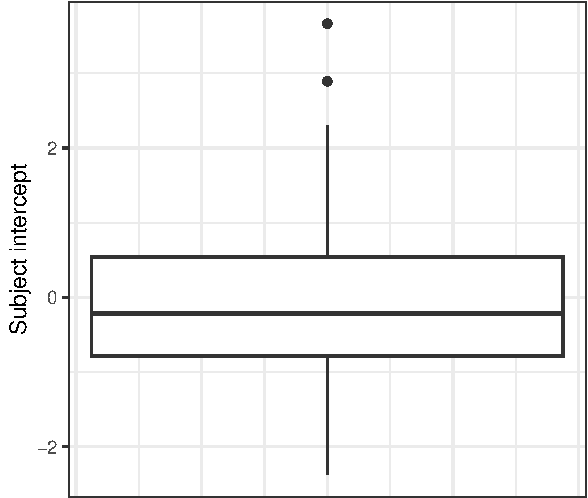
\includegraphics{4_files/figure-pdf/fig-random-subject-var-1.pdf}

}

\caption{\label{fig-random-subject-var}Distribución de interceptos
aleatorios en el modelo Response \textasciitilde{} Treat * Period + (1
\textbar{} Subject)}

\end{figure}

\hypertarget{modelo-response-treat-period-1-treat-subject}{%
\subsubsection{Modelo Response \textasciitilde{} Treat * Period + (1 +
Treat \textbar{}
Subject)}\label{modelo-response-treat-period-1-treat-subject}}

Es posible que cada estudiante valore con diferente criterio cada
subtitulado. Para estimarlo, se propone el siguiente modelo:

\small

\[
\begin{aligned}
Level\ 1: & \text{logit}(P(Response_{ij} \leq k)) = \tau_{kj} - \beta_{1j} \text{Treat}_{ij} - \beta_{2} \text{Period}_{ij} - \beta_{3} \text{Treat}_{ij} * \text{Period}_{ij} \\
Level\ 2: & \tau_{kj}  =  \tau_{k} + U_{0j} \\
          & \beta_{1j}  =  \beta_{1} + U_{1j}
\end{aligned}
\]

\normalsize

Ahora el parámetro \(\beta_{1j}\) del subtitulado tiene dos componentes:
Uno común a todos los estudiantes \(\beta_{1}\) y otro particular de
cada estudiante \(U_{1j}\). El modelo ajustado ocasiona que solo
\texttt{Treat1} sea significativo, ya que ni el periodo ni la secuencia
lo son. En los efectos aleatorios la correlación entre intercepto y
pendiente es prácticamente nula.

\scriptsize

\begin{Shaded}
\begin{Highlighting}[]
\FunctionTok{options}\NormalTok{(}\AttributeTok{contrasts =} \FunctionTok{rep}\NormalTok{(}\StringTok{"contr.sum"}\NormalTok{, }\DecValTok{2}\NormalTok{))}
\NormalTok{clmm\_treat.period\_treat.subject }\OtherTok{\textless{}{-}} \FunctionTok{clmm}\NormalTok{(}
\NormalTok{    Response }\SpecialCharTok{\textasciitilde{}}\NormalTok{ Treat }\SpecialCharTok{*}\NormalTok{ Period }\SpecialCharTok{+}\NormalTok{ (}\DecValTok{1} \SpecialCharTok{+}\NormalTok{ Treat }\SpecialCharTok{|}\NormalTok{ Subject),}
    \AttributeTok{data =}\NormalTok{ df\_clean}
\NormalTok{)}
\FunctionTok{summary}\NormalTok{(clmm\_treat.period\_treat.subject)}
\end{Highlighting}
\end{Shaded}

\begin{verbatim}
Cumulative Link Mixed Model fitted with the Laplace approximation

formula: Response ~ Treat * Period + (1 + Treat | Subject)
data:    df_clean

 link  threshold nobs logLik   AIC     niter     max.grad cond.H 
 logit flexible  2980 -3429.88 6879.76 905(6264) 1.33e-03 8.2e+01

Random effects:
 Groups  Name        Variance Std.Dev. Corr   
 Subject (Intercept) 1.712    1.308           
         Treat1      1.042    1.021    -0.062 
Number of groups:  Subject 87 

Coefficients:
               Estimate Std. Error z value Pr(>|z|)    
Treat1           1.2938     0.1197  10.809   <2e-16 ***
Period1          0.1620     0.1171   1.383    0.167    
Treat1:Period1   0.1327     0.1464   0.906    0.365    
---
Signif. codes:  0 '***' 0.001 '**' 0.01 '*' 0.05 '.' 0.1 ' ' 1

Threshold coefficients:
    Estimate Std. Error z value
1|2  -4.2633     0.1761 -24.210
2|3  -2.3321     0.1562 -14.932
3|4  -1.2656     0.1520  -8.324
4|5   0.9659     0.1509   6.400
\end{verbatim}

\normalsize

\hypertarget{comparaciuxf3n-de-modelos}{%
\subsubsection{Comparación de modelos}\label{comparaciuxf3n-de-modelos}}

Se pueden comparar los modelos con el test de razón de verosimilitud que
se realiza con la función \texttt{anova} del paquete \texttt{ordinal}.
Se comprueba que en este test resulta significativamente mejor el último
modelo:

\scriptsize

\begin{Shaded}
\begin{Highlighting}[]
\FunctionTok{anova}\NormalTok{(clmm\_treat.period\_subject, clmm\_treat.period\_treat.subject)}
\end{Highlighting}
\end{Shaded}

\begin{verbatim}
Likelihood ratio tests of cumulative link models:
 
                                formula:                                         
clmm_treat.period_subject       Response ~ Treat * Period + (1 | Subject)        
clmm_treat.period_treat.subject Response ~ Treat * Period + (1 + Treat | Subject)
                                link: threshold:
clmm_treat.period_subject       logit flexible  
clmm_treat.period_treat.subject logit flexible  

                                no.par    AIC  logLik LR.stat df Pr(>Chisq)    
clmm_treat.period_subject            8 7327.4 -3655.7                          
clmm_treat.period_treat.subject     10 6879.8 -3429.9  451.66  2  < 2.2e-16 ***
---
Signif. codes:  0 '***' 0.001 '**' 0.01 '*' 0.05 '.' 0.1 ' ' 1
\end{verbatim}

\normalsize

\hypertarget{elecciuxf3n-del-mejor-modelo}{%
\subsubsection{Elección del mejor
modelo}\label{elecciuxf3n-del-mejor-modelo}}

Se han comparado distintos modelos:

\begin{itemize}
\tightlist
\item
  Response \textasciitilde{} (1 \textbar{} Subject)
\item
  Response \textasciitilde{} (1 + Treat \textbar{} Subject)
\item
  Response \textasciitilde{} (1 + Treat \textbar{} Question)
\item
  Response \textasciitilde{} Treat + (1 + Treat \textbar{} Subject)
\item
  Response \textasciitilde{} Treat + (1 + Treat \textbar{} Question)
\item
  Response \textasciitilde{} Treat*Period + (1 + Treat \textbar{}
  Subject)
\item
  Response \textasciitilde{} Treat*Period + (1 + Treat \textbar{}
  Question)
\item
  Response \textasciitilde{} Treat*Period + (1 + Period \textbar{}
  Subject) + (1 + Treat \textbar{} Question)
\item
  Response \textasciitilde{} Treat + (1 + Treat \textbar{} Subject) + (1
  + Treat \textbar{} Question)
\item
  Response \textasciitilde{} Treat*Period + (1 + Treat \textbar{}
  Subject) + (1 + Treat \textbar{} Question)
\end{itemize}

El último de ellos produce un resultado significativo en el test de
razón de verosimilitud con todos los demás. Sin embargo los parámetros
de todos los modelos tienen valores similares por lo que no cambia la
interpretación que se haga de ellos en cada modelo. Este modelo tiene un
\(AIC\) menor que los modelos ordinales ajustados en el apartado
anterior (ver Sección~\ref{sec-ordinal-2}) incluso si a esos modelos se
les añade como factor predictor \texttt{Question}. En la
Figura~\ref{fig-probs-clmm_treat.period.subject.question} se muestran
las predicciones del modelo. El resumen de parámetros del modelo es el
siguiente:

\scriptsize

\begin{Shaded}
\begin{Highlighting}[]
\FunctionTok{options}\NormalTok{(}\AttributeTok{contrasts =} \FunctionTok{rep}\NormalTok{(}\StringTok{"contr.sum"}\NormalTok{, }\DecValTok{2}\NormalTok{))}
\NormalTok{clmm\_treat.period.subject.question }\OtherTok{\textless{}{-}} \FunctionTok{clmm}\NormalTok{(}
\NormalTok{    Response }\SpecialCharTok{\textasciitilde{}}\NormalTok{ Treat }\SpecialCharTok{*}\NormalTok{ Period }\SpecialCharTok{+}\NormalTok{ (}\DecValTok{1} \SpecialCharTok{+}\NormalTok{ Treat }\SpecialCharTok{|}\NormalTok{ Subject) }\SpecialCharTok{+}\NormalTok{ (}\DecValTok{1} \SpecialCharTok{+}\NormalTok{ Treat }\SpecialCharTok{|}\NormalTok{ Question),}
    \AttributeTok{data =}\NormalTok{ df\_clean}
\NormalTok{)}
\FunctionTok{summary}\NormalTok{(clmm\_treat.period.subject.question)}
\end{Highlighting}
\end{Shaded}

\begin{verbatim}
Cumulative Link Mixed Model fitted with the Laplace approximation

formula: Response ~ Treat * Period + (1 + Treat | Subject) + (1 + Treat |  
    Question)
data:    df_clean

 link  threshold nobs logLik   AIC     niter       max.grad cond.H 
 logit flexible  2980 -3186.06 6398.11 1468(12273) 2.37e-03 1.5e+02

Random effects:
 Groups   Name        Variance Std.Dev. Corr   
 Subject  (Intercept) 2.2176   1.4892          
          Treat1      1.3650   1.1683   -0.128 
 Question (Intercept) 0.4831   0.6950          
          Treat1      0.4655   0.6823   -0.528 
Number of groups:  Subject 87,  Question 18 

Coefficients:
               Estimate Std. Error z value Pr(>|z|)    
Treat1           1.4320     0.2102   6.811  9.7e-12 ***
Period1          0.1730     0.1325   1.306    0.192    
Treat1:Period1   0.1397     0.1654   0.845    0.398    
---
Signif. codes:  0 '***' 0.001 '**' 0.01 '*' 0.05 '.' 0.1 ' ' 1

Threshold coefficients:
    Estimate Std. Error z value
1|2  -5.0033     0.2619 -19.104
2|3  -2.6499     0.2417 -10.962
3|4  -1.3659     0.2376  -5.748
4|5   1.1837     0.2365   5.006
\end{verbatim}

\normalsize

Las ecuaciones del modelo están en Ecuación~\ref{eq-mejor-modelo}.

\small

\begin{equation}\protect\hypertarget{eq-mejor-modelo}{}{
\begin{aligned}
Level\ 1: & \text{logit}(P(Response_{ijl} \leq k)) = \tau_{kjl} - \beta_{1jl} \text{Treat}_{ijl} - \beta_{2} \text{Period}_{ijl} - \beta_{3} \text{Treat}_{ijl} * \text{Period}_{ijl} \\
Level\ 2: & \tau_{kjl}  =  \tau_{k} + U_{0j} + V_{0l} \\
          & \beta_{1jl}  =  \beta_{1} + U_{1j} + V_{1l}
\end{aligned}
}\label{eq-mejor-modelo}\end{equation}

\normalsize

donde \(ijk\) se corresponde con la observación \(i\)-ésima del
estudiante \(j\) y nivel de subtitulado \(k\). Ahora los interceptos y
el coeficiente del subtitulado se componen de tres sumandos: una parte
fija, una parte que depende del estudiante y una parte que depende del
nivel de subtitulado.

\begin{figure}[h]

{\centering 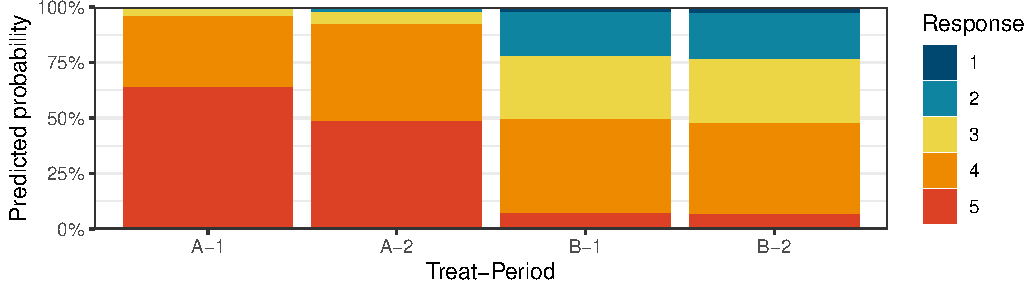
\includegraphics{4_files/figure-pdf/fig-probs-clmm_treat.period.subject.question-1.pdf}

}

\caption{\label{fig-probs-clmm_treat.period.subject.question}Probabilidades
de respuesta para el modelo ordinal Response \textasciitilde{} Treat *
Period + (1 + Treat \textbar{} Subject) + (1 + Treat \textbar{}
Question)}

\end{figure}

\hypertarget{sec-bayesiano-2}{%
\subsection{Modelado bayesiano}\label{sec-bayesiano-2}}

Existen muchos paquetes en R para hacer inferencia bayesiana. Algunos de
ellos son:

\begin{itemize}
\tightlist
\item
  OpenBUGS y WinBUGS: basado en el muestreo de Gibbs.
\item
  JAGS: también utiliza el muestreo de Gibbs.
\item
  Stan: Más moderna y con una comunidad de desarrollo más activa que los
  anteriores. Utiliza muestreo HMC (Hamiltonian Monte Carlo) y NUTS (no
  U-turn sampler). Se pueden definir modelos directamente con el
  lenguaje de modelado de Stan. Hay muchos paquetes basados en Stan que
  facilitan la especificación de modelos con una sintaxis más sencilla.
  En este trabajo se utilizará uno de ellos, \(brms\).
\item
  INLA: Evita la simulación MCMC haciendo más rápida la convergencia. Es
  menos flexible ya que solo se pueden especificar modelos de la familia
  exponencial.
\end{itemize}

Se han comparado múltiples modelos usando la función \texttt{LOO} que
realiza una validación cruzada bayesiana \texttt{leave-one-out} similar
a la que se explicó en la Sección~\ref{sec-bayesiano}. El mejor modelo
ha resultado ser el mismo que se seleccionó en modelos mixtos (ver
Ecuación~\ref{eq-mejor-modelo}). Es decir:

\small

\begin{quote}
Response \textasciitilde{} Treat*Period + (1 + Treat \textbar{} Subject)
+ (1 + Treat \textbar{} Question) \normalsize
\end{quote}

\scriptsize

\begin{Shaded}
\begin{Highlighting}[]
\FunctionTok{options}\NormalTok{(}\AttributeTok{contrasts =} \FunctionTok{rep}\NormalTok{(}\StringTok{"contr.sum"}\NormalTok{, }\DecValTok{2}\NormalTok{))}
\NormalTok{brm\_treat.period.subject.question }\OtherTok{\textless{}{-}} \FunctionTok{brm}\NormalTok{(}
\NormalTok{    Response }\SpecialCharTok{\textasciitilde{}}\NormalTok{ Treat }\SpecialCharTok{*}\NormalTok{ Period }\SpecialCharTok{+}\NormalTok{ (}\DecValTok{1} \SpecialCharTok{+}\NormalTok{ Treat }\SpecialCharTok{|}\NormalTok{ Subject) }\SpecialCharTok{+}\NormalTok{ (}\DecValTok{1} \SpecialCharTok{+}\NormalTok{ Treat }\SpecialCharTok{|}\NormalTok{ Question),}
    \AttributeTok{data =}\NormalTok{ df\_clean,}
    \AttributeTok{family =} \FunctionTok{cumulative}\NormalTok{(}\StringTok{"logit"}\NormalTok{),}
    \AttributeTok{iter =} \DecValTok{4000}\NormalTok{,}
    \AttributeTok{sample\_prior =} \ConstantTok{TRUE}\NormalTok{,}
    \AttributeTok{file =} \StringTok{"models/brm\_treat.period.subject.question"}\NormalTok{,}
    \AttributeTok{file\_refit =} \StringTok{"on\_change"}
\NormalTok{)}
\end{Highlighting}
\end{Shaded}

\normalsize

El modelo utiliza como factores con efectos fijos
(\texttt{complete\ pooling} en terminología bayesiana) el nivel de
subtitulado y el periodo y la interacción entre ambos; y como efectos
aleatorios (\texttt{partial\ pooling}) los sujetos y las preguntas del
test, cada uno de ellos con un intercepto y un nivel de subtitulado
variable. El resumen del modelo es el siguiente:

\tiny

\begin{Shaded}
\begin{Highlighting}[]
\FunctionTok{summary}\NormalTok{(brm\_treat.period.subject.question)}
\end{Highlighting}
\end{Shaded}

\begin{verbatim}
 Family: cumulative 
  Links: mu = logit; disc = identity 
Formula: Response ~ Treat * Period + (1 + Treat | Subject) + (1 + Treat | Question) 
   Data: df_clean (Number of observations: 2980) 
  Draws: 4 chains, each with iter = 4000; warmup = 2000; thin = 1;
         total post-warmup draws = 8000

Group-Level Effects: 
~Question (Number of levels: 18) 
                      Estimate Est.Error l-95% CI u-95% CI Rhat Bulk_ESS
sd(Intercept)             0.78      0.15     0.54     1.13 1.00     1873
sd(Treat1)                0.76      0.15     0.53     1.12 1.01     1708
cor(Intercept,Treat1)    -0.46      0.20    -0.79    -0.00 1.00     1738
                      Tail_ESS
sd(Intercept)             3754
sd(Treat1)                3645
cor(Intercept,Treat1)     2863

~Subject (Number of levels: 87) 
                      Estimate Est.Error l-95% CI u-95% CI Rhat Bulk_ESS
sd(Intercept)             1.54      0.14     1.30     1.83 1.00     1339
sd(Treat1)                1.21      0.11     1.02     1.45 1.00     1644
cor(Intercept,Treat1)    -0.11      0.13    -0.36     0.13 1.00     1213
                      Tail_ESS
sd(Intercept)             3047
sd(Treat1)                3421
cor(Intercept,Treat1)     2301

Population-Level Effects: 
               Estimate Est.Error l-95% CI u-95% CI Rhat Bulk_ESS Tail_ESS
Intercept[1]      -4.96      0.27    -5.50    -4.42 1.00      985     1681
Intercept[2]      -2.60      0.26    -3.09    -2.11 1.00      899     1788
Intercept[3]      -1.32      0.25    -1.80    -0.82 1.00      876     1748
Intercept[4]       1.24      0.25     0.76     1.74 1.00      872     1775
Treat1             1.45      0.23     1.01     1.93 1.00     1229     2318
Period1            0.17      0.14    -0.10     0.43 1.00     1004     2236
Treat1:Period1     0.14      0.17    -0.19     0.47 1.01      698     1414

Family Specific Parameters: 
     Estimate Est.Error l-95% CI u-95% CI Rhat Bulk_ESS Tail_ESS
disc     1.00      0.00     1.00     1.00   NA       NA       NA

Draws were sampled using sampling(NUTS). For each parameter, Bulk_ESS
and Tail_ESS are effective sample size measures, and Rhat is the potential
scale reduction factor on split chains (at convergence, Rhat = 1).
\end{verbatim}

\normalsize

Se han mantenido las distribuciones de probabilidad a priori que por
defecto utiliza \texttt{brm} confiando en que sus parámetros son
adecuados. Sin embargo, conviene comprobar que realmente sea así. En la
Tabla~\ref{tbl-priors} se muestran las distribuciones a priori de los
parámetros aleatorios del modelo. En la Figura~\ref{fig-priors} se
constata que toman valores razonables y no informativos.

\tiny

\hypertarget{tbl-priors}{}
\begin{longtable}{llllrrrrrl}
\caption{\label{tbl-priors}Distribuciones a priori del modelo Response \textasciitilde{} Treat *
Period + (1 + Treat \textbar{} Subject) + (1 + Treat \textbar{}
Question). }\tabularnewline

\toprule
prior & class & coef & group & resp & dpar & nlpar & lb & ub & source \\ 
\midrule
 & b &  &  &  &  &  &  &  & default \\ 
 & b & Period1 &  &  &  &  &  &  & default \\ 
 & b & Treat1 &  &  &  &  &  &  & default \\ 
 & b & Treat1:Period1 &  &  &  &  &  &  & default \\ 
student\_t(3, 0, 2.5) & Intercept &  &  &  &  &  &  &  & default \\ 
student\_t(3, 0, 2.5) & Intercept & 1 &  &  &  &  &  &  & default \\ 
student\_t(3, 0, 2.5) & Intercept & 2 &  &  &  &  &  &  & default \\ 
student\_t(3, 0, 2.5) & Intercept & 3 &  &  &  &  &  &  & default \\ 
student\_t(3, 0, 2.5) & Intercept & 4 &  &  &  &  &  &  & default \\ 
lkj\_corr\_cholesky(1) & L &  &  &  &  &  &  &  & default \\ 
lkj\_corr\_cholesky(1) & L &  & Question &  &  &  &  &  & default \\ 
lkj\_corr\_cholesky(1) & L &  & Subject &  &  &  &  &  & default \\ 
student\_t(3, 0, 2.5) & sd &  &  &  &  &  & 0 &  & default \\ 
student\_t(3, 0, 2.5) & sd &  & Question &  &  &  &  &  & default \\ 
student\_t(3, 0, 2.5) & sd & Intercept & Question &  &  &  &  &  & default \\ 
student\_t(3, 0, 2.5) & sd & Treat1 & Question &  &  &  &  &  & default \\ 
student\_t(3, 0, 2.5) & sd &  & Subject &  &  &  &  &  & default \\ 
student\_t(3, 0, 2.5) & sd & Intercept & Subject &  &  &  &  &  & default \\ 
student\_t(3, 0, 2.5) & sd & Treat1 & Subject &  &  &  &  &  & default \\ 
\bottomrule
\end{longtable}

\normalsize

\begin{figure}[h]

{\centering 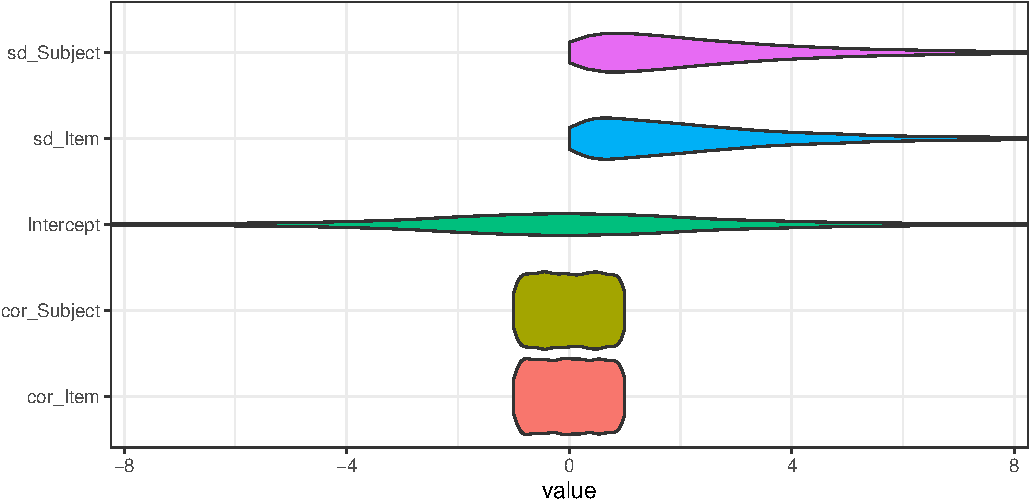
\includegraphics{4_files/figure-pdf/fig-priors-1.pdf}

}

\caption{\label{fig-priors}Distribuciones a priori del modelo Response
\textasciitilde{} Treat * Period + (1 + Treat \textbar{} Subject) + (1 +
Treat \textbar{} Question).}

\end{figure}

Es importante asegurar que el entrenamiento ha convergido a su
distribución a posteriori. En la tabla de resumen constatamos que el
valor de \texttt{Rhat} es inferior a 1.1 y el de \texttt{ESS} superior a
400 en todos los parámetros, que son umbrales que no se deberían violar
\autocite[ver][]{burkner2019}. En la Figura~\ref{fig-trace} se comprueba
que las cadenas MCMC de muestreo de la distribución a posteriori se
mezclan correctamente y no se aprecia autocorrelación en ninguno de las
parámetros. Por último, en la Figura~\ref{fig-predictive} se muestra una
comparación entre los histogramas construidos con los datos con los
intervalos de confianza marginales de la función predictiva a posteriori
del modelo. En la mayoría de las preguntas, el muestreo reproduce
bastante bien el histograma de respuestas, aunque en algunas preguntas,
como la \texttt{Q16} o la \texttt{Q17}, se aprecian diferencias
relevantes.

\begin{figure}[h]

{\centering 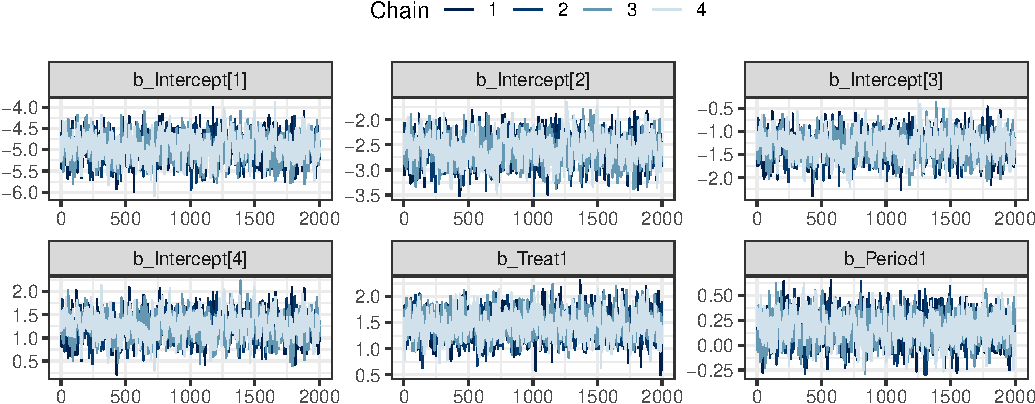
\includegraphics{4_files/figure-pdf/fig-trace-1.pdf}

}

\caption{\label{fig-trace}Cadenas MCMC del modelo Response
\textasciitilde{} Treat * Period + (1 + Treat \textbar{} Subject) + (1 +
Treat \textbar{} Question).}

\end{figure}

\begin{figure}[h]

{\centering 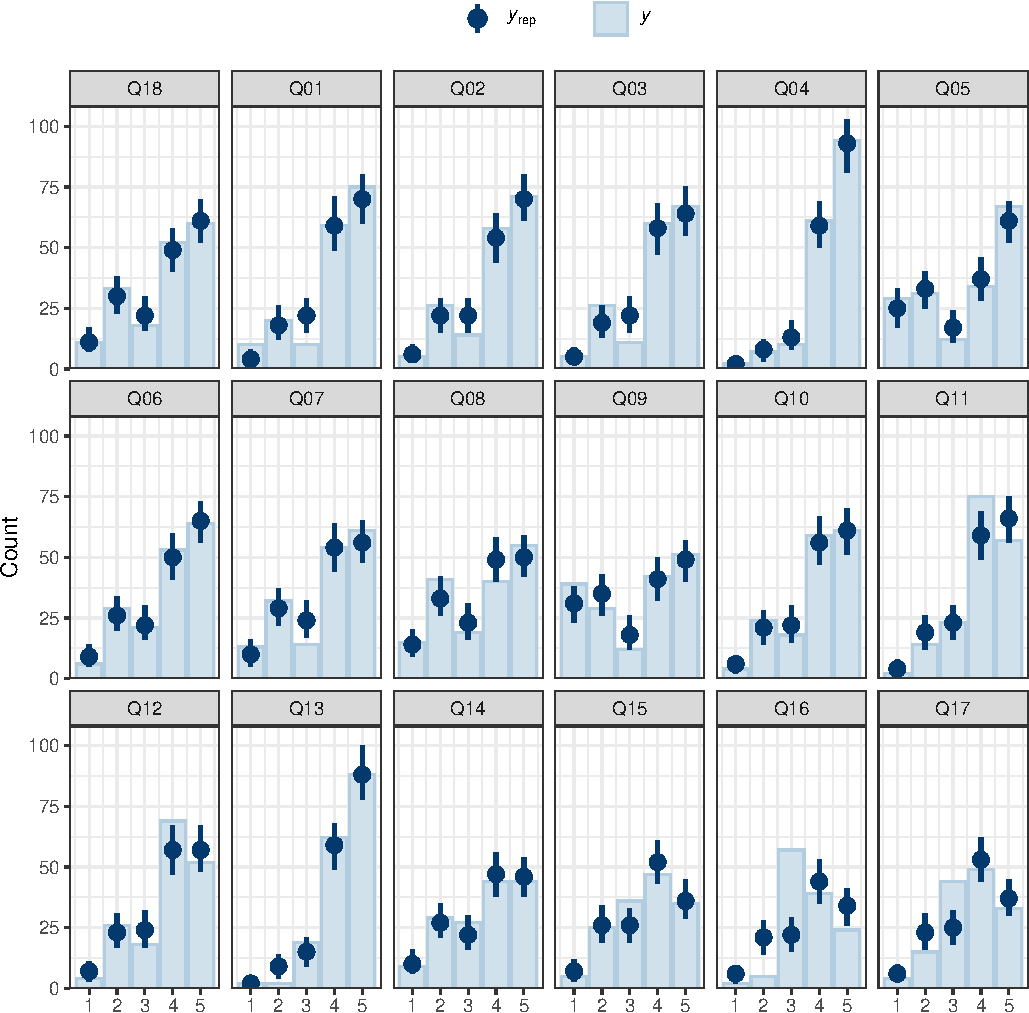
\includegraphics{4_files/figure-pdf/fig-predictive-1.pdf}

}

\caption{\label{fig-predictive}Comparación de los valores reales con los
obtenidos a partir de la función predictiva a posteriori del modelo
Response \textasciitilde{} Treat * Period + (1 + Treat \textbar{}
Subject) + (1 + Treat \textbar{} Question).}

\end{figure}

\bookmarksetup{startatroot}

\hypertarget{section}{%
\chapter{}\label{section}}

\bookmarksetup{startatroot}

\hypertarget{section-1}{%
\chapter{}\label{section-1}}

\bookmarksetup{startatroot}

\hypertarget{section-2}{%
\chapter{}\label{section-2}}

\bookmarksetup{startatroot}

\hypertarget{section-3}{%
\chapter{}\label{section-3}}

\bookmarksetup{startatroot}

\hypertarget{section-4}{%
\chapter{}\label{section-4}}

\bookmarksetup{startatroot}

\hypertarget{section-5}{%
\chapter{}\label{section-5}}

\bookmarksetup{startatroot}

\hypertarget{section-6}{%
\chapter{}\label{section-6}}

\bookmarksetup{startatroot}

\hypertarget{section-7}{%
\chapter{}\label{section-7}}

\bookmarksetup{startatroot}

\hypertarget{section-8}{%
\chapter{}\label{section-8}}

\bookmarksetup{startatroot}

\hypertarget{section-9}{%
\chapter{}\label{section-9}}

\bookmarksetup{startatroot}

\hypertarget{section-10}{%
\chapter{}\label{section-10}}

\bookmarksetup{startatroot}

\hypertarget{sec-resultados}{%
\chapter{Resultados}\label{sec-resultados}}

En esté capítulo se comentarán los resultados de las técnicas
estadísticas y de los modelos propuestos (ver
Capítulo~\ref{sec-modelado}).

\hypertarget{sec-cronbach-2}{%
\subsection{Correlación entre preguntas con el alfa de
Cronbach}\label{sec-cronbach-2}}

\scriptsize

\normalsize

El coeficiente \texttt{alfa\ de\ Cronbach} (ver
Sección~\ref{sec-cronbach}) de la escala de Likert es 0.921 lo que
indica una muy buena correlación entre las respuestas a todas los ítems.
Este valor apenas se ve alterado si se elimina una de ellos. Esto nos
permite concluir que todos los ítems pertenecen a la misma escala de
Likert. En la Tabla~\ref{tbl-item-alpha} mostramos los ítems que más
contribuyen al índice \texttt{alpha\ de\ Cronbach}. Un resultado
interesante es constatar que el ítem \(Q18\), que es la valoración
general del cuestionario, es el que mejor contribución tiene al índice.

\tiny

\begin{table}

\caption{\label{tbl-item-alpha}Relación de cada ítem con el índice alpha
de Cronbach.}\begin{minipage}[t]{\linewidth}
\subcaption{\label{tbl-item-alpha-1}Variables con mayor asociación. }

{\centering 

\begin{longtable}{rrrrrrrrr}
\tabularnewline

\toprule
Q18 & Q05 & Q06 & Q09 & Q08 & Q07 & Q10 & Q12 & Q02 \\ 
\midrule
0.86 & 0.81 & 0.79 & 0.79 & 0.77 & 0.75 & 0.73 & 0.72 & 0.71 \\ 
\bottomrule
\end{longtable}

}

\end{minipage}%
\newline
\begin{minipage}[t]{\linewidth}
\subcaption{\label{tbl-item-alpha-2}Variables con menor asociación. }

{\centering 

\begin{longtable}{rrrrrrrrr}
\tabularnewline

\toprule
Q03 & Q14 & Q01 & Q11 & Q15 & Q13 & Q04 & Q16 & Q17 \\ 
\midrule
0.68 & 0.66 & 0.65 & 0.64 & 0.56 & 0.51 & 0.46 & 0.44 & 0.42 \\ 
\bottomrule
\end{longtable}

}

\end{minipage}%

\end{table}

\normalsize

\hypertarget{sec-chi2-2}{%
\subsection{\texorpdfstring{Asociación de variables con la prueba de
homogeneidad
\emph{X²}}{Asociación de variables con la prueba de homogeneidad X²}}\label{sec-chi2-2}}

En la Sección~\ref{sec-chi2} se describe el marco teórico de esta prueba
no paramétrica. Se ha contrastado la existencia de asociación entre la
variable respuesta \(Response\) y cada una de las tres variables más
importantes de nuestro modelo (\(Treat\), \(Period\) y \(Seq\)). En la
Tabla~\ref{tbl-contingencia-2} se muestran las tablas de contingencia.
La Tabla~\ref{tbl-chi2} permite comprobar que todos los contrastes son
significativos, con lo que se rechaza la hipótesis nula de homogeneidad.
Todas las variables explicativas tienen influencia en la variable
respuesta.

\begin{table}

\caption{\label{tbl-contingencia-2}Tablas de
contingencia.}\begin{minipage}[t]{0.33\linewidth}
\subcaption{\label{tbl-contingencia-2-1}Response + Treat }

{\centering 

\tabularnewline

\centering
\begin{tabular}{l|r|r}
\hline
Response & A & B\\
\hline
1 & 4 & 163\\
\hline
2 & 55 & 359\\
\hline
3 & 135 & 248\\
\hline
4 & 548 & 409\\
\hline
5 & 755 & 304\\
\hline
\end{tabular}

}

\end{minipage}%
%
\begin{minipage}[t]{0.33\linewidth}
\subcaption{\label{tbl-contingencia-2-2}Response + Period }

{\centering 

\tabularnewline

\centering
\begin{tabular}{r|r}
\hline
1 & 2\\
\hline
78 & 89\\
\hline
199 & 215\\
\hline
198 & 185\\
\hline
440 & 517\\
\hline
572 & 487\\
\hline
\end{tabular}

}

\end{minipage}%
%
\begin{minipage}[t]{0.33\linewidth}
\subcaption{\label{tbl-contingencia-2-3}Response + Seq }

{\centering 

\tabularnewline

\centering
\begin{tabular}{r|r}
\hline
AB & BA\\
\hline
89 & 78\\
\hline
210 & 204\\
\hline
192 & 191\\
\hline
375 & 582\\
\hline
600 & 459\\
\hline
\end{tabular}

}

\end{minipage}%

\end{table}

\hypertarget{tbl-chi2}{}
\begin{longtable}[]{@{}
  >{\raggedright\arraybackslash}p{(\columnwidth - 6\tabcolsep) * \real{0.1100}}
  >{\raggedleft\arraybackslash}p{(\columnwidth - 6\tabcolsep) * \real{0.2900}}
  >{\raggedleft\arraybackslash}p{(\columnwidth - 6\tabcolsep) * \real{0.3000}}
  >{\raggedleft\arraybackslash}p{(\columnwidth - 6\tabcolsep) * \real{0.3000}}@{}}
\caption{\label{tbl-chi2}Valores del contraste de hipótesis
\(\chi^2\)}\tabularnewline
\toprule\noalign{}
\begin{minipage}[b]{\linewidth}\raggedright
\end{minipage} & \begin{minipage}[b]{\linewidth}\raggedleft
\textasciitilde{} Response + Treat
\end{minipage} & \begin{minipage}[b]{\linewidth}\raggedleft
\textasciitilde{} Response + Period
\end{minipage} & \begin{minipage}[b]{\linewidth}\raggedleft
\textasciitilde{} Response + Seq
\end{minipage} \\
\midrule\noalign{}
\endfirsthead
\toprule\noalign{}
\begin{minipage}[b]{\linewidth}\raggedright
\end{minipage} & \begin{minipage}[b]{\linewidth}\raggedleft
\textasciitilde{} Response + Treat
\end{minipage} & \begin{minipage}[b]{\linewidth}\raggedleft
\textasciitilde{} Response + Period
\end{minipage} & \begin{minipage}[b]{\linewidth}\raggedleft
\textasciitilde{} Response + Seq
\end{minipage} \\
\midrule\noalign{}
\endhead
\bottomrule\noalign{}
\endlastfoot
\(\chi^2\) & 621.497 & 15.039 & 64.904 \\
\(p\)-value & \ensuremath{4.5778215\times 10^{-132}} & 0.0101975 &
\ensuremath{1.1733569\times 10^{-12}} \\
\(df\) & 5 & 5 & 5 \\
\end{longtable}

\hypertarget{sec-or-3}{%
\subsection{\texorpdfstring{Comparación con \emph{Odds
Ratio}}{Comparación con Odds Ratio}}\label{sec-or-3}}

En Sección~\ref{sec-or} y en Sección~\ref{sec-or-2} se exponen el marco
teórico y la fundamentación de los contrastes de hipótesis realizados
respectivamente. El contraste de hipótesis del \(log\ OR\) del
subtitulado para cada grupo no produce significación estadística en
ningún nivel de respuesta, por lo que según esta prueba estadística la
secuencia de subtitulado no influiría en la respuesta de los estudiantes
(ver Tabla~\ref{tbl-logor1}). Es decir, de acuerdo a este test la
secuencia no influye en la valoración de los subtítulos.

\hypertarget{tbl-logor1}{}
\begin{longtable}{lrrrr}
\caption{\label{tbl-logor1}\(Log OR\) \textasciitilde{} Treat + Seq + Response\_l }\tabularnewline

\toprule
Response & Estimate & Std. Error & z value & Pr(>|z|) \\ 
\midrule
No sé / No contesto & 0.190 & 0.327 & 0.580 & 0.562 \\ 
Muy en desacuerdo & -0.135 & 1.012 & -0.134 & 0.894 \\ 
En desacuerdo & -0.244 & 0.291 & -0.838 & 0.402 \\ 
Neutral & 0.152 & 0.214 & 0.711 & 0.477 \\ 
De acuerdo & -0.210 & 0.134 & -1.570 & 0.116 \\ 
Muy de acuerdo & 0.117 & 0.137 & 0.855 & 0.393 \\ 
\bottomrule
\end{longtable}

Sin embargo, si realizamos este contraste entre subtítulos y periodos
podemos constatar la existencia de un efecto periodo de signo contrario
para las preguntas 4 y 5 (ver Tabla~\ref{tbl-logor2}).

\hypertarget{tbl-logor2}{}
\begin{longtable}{lrrrr}
\caption{\label{tbl-logor2}Log OR \textasciitilde{} Treat + Period + Response\_l }\tabularnewline

\toprule
Response & Estimate & Std. Error & z value & Pr(>|z|) \\ 
\midrule
No sé / No contesto & 0.335 & 0.327 & 1.022 & 0.307 \\ 
Muy en desacuerdo & 0.135 & 1.012 & 0.134 & 0.894 \\ 
En desacuerdo & -0.121 & 0.291 & -0.416 & 0.677 \\ 
Neutral & 0.055 & 0.214 & 0.259 & 0.796 \\ 
De acuerdo & -0.851 & 0.134 & -6.367 & 0.000 \\ 
Muy de acuerdo & 0.486 & 0.137 & 3.557 & 0.000 \\ 
\bottomrule
\end{longtable}

\hypertarget{modelado}{%
\subsection{Modelado}\label{modelado}}

El modelo de efectos mixtos ajustado con Regresión Logística:

\begin{quote}
Improve \textasciitilde{} 1 + (1 \textbar{} Subject) + (1 \textbar{}
Question)
\end{quote}

estima la probabilidad de que la respuesta a un ítem en el subtitulado
\(A\) sea mejor que en el subtitulado \(B\) frente a que sea igual o
peor. El intercepto del modelo ajustado es 0.404. Por ello, la
probabilidad de que se otorgue una mayor puntuación en \(A\) que en
\(B\) es del 59.95\%. En la Tabla~\ref{tbl-improve-question} se muestra
la probabilidad de que la respuesta sea mejor en \(A\) que en \(B\) por
ítem.

\scriptsize

\hypertarget{tbl-improve-question}{}
\begin{longtable}{lr}
\caption{\label{tbl-improve-question}Probabilidad de que la respuesta a un ítem sea A \textgreater{} B frente
a A \textless= B }\tabularnewline

\toprule
Question & Prob \\ 
\midrule
Q18 & $0.70$ \\ 
Q01 & $0.36$ \\ 
Q02 & $0.57$ \\ 
Q03 & $0.38$ \\ 
Q04 & $0.16$ \\ 
Q05 & $0.81$ \\ 
Q06 & $0.68$ \\ 
Q07 & $0.58$ \\ 
Q08 & $0.68$ \\ 
Q09 & $0.86$ \\ 
Q10 & $0.45$ \\ 
Q11 & $0.40$ \\ 
Q12 & $0.50$ \\ 
Q13 & $0.24$ \\ 
Q14 & $0.64$ \\ 
Q15 & $0.30$ \\ 
Q16 & $0.24$ \\ 
Q17 & $0.33$ \\ 
\bottomrule
\end{longtable}

\normalsize

En la Sección~\ref{sec-ordinal-2} se evaluaron distintas
parametrizaciones de la Regresión Ordinal Acumulativa tanto desde el
punto de vista frecuentista como bayesiano y considerando únicamente
efectos fijos y también efectos aleatorios. Finalmente, tanto en el
análisis frecuentista como en el bayesiano, el modelo que resultó ser
más parsimonioso es el de la Ecuación~\ref{eq-mejor-modelo}, que se
reproduce aquí en sintaxis R:

\small

\begin{quote}
Response \textasciitilde{} Treat*Period + (1 + Treat \textbar{} Subject)
+ (1 + Treat \textbar{} Question) \normalsize
\end{quote}

Este modelo produce en los dos paradigmas unas estimaciones similares,
como se puede comprobar en la Tabla~\ref{tbl-model-comp}.

\tiny

\hypertarget{tbl-model-comp}{}
\begin{longtable}{lrrrrrr}
\caption{\label{tbl-model-comp}Comparación frecuentista/bayesiano de coeficientes estimados en el
modelo Response \textasciitilde{} Treat * Period + (1 + Treat \textbar{}
Subject) + (1 + Treat \textbar{} Question). }\tabularnewline

\toprule
 & \multicolumn{3}{c}{ordinal::clmm} & \multicolumn{3}{c}{brms::brm} \\ 
\cmidrule(lr){2-4} \cmidrule(lr){5-7}
Name & Estimation.clmm & conf.2.5\% & conf.97.5\% & Estimation.brm & cred.2.5\% & cred.97.5\% \\ 
\midrule
1|2 & -5.00 & -5.52 & -4.49 & -4.96 & -5.50 & -4.42 \\ 
2|3 & -2.65 & -3.12 & -2.18 & -2.60 & -3.09 & -2.11 \\ 
3|4 & -1.37 & -1.83 & -0.90 & -1.32 & -1.80 & -0.82 \\ 
4|5 & 1.18 & 0.72 & 1.65 & 1.24 & 0.76 & 1.74 \\ 
Treat1 & 1.43 & 1.02 & 1.84 & 1.45 & 1.01 & 1.93 \\ 
Period1 & 0.17 & -0.09 & 0.43 & 0.17 & -0.10 & 0.43 \\ 
Treat1:Period1 & 0.14 & -0.18 & 0.46 & 0.14 & -0.19 & 0.47 \\ 
Question.sd(Intercept) & 0.70 &  &  & 0.76 & 0.54 & 1.13 \\ 
Question.sd(Treat1) & 0.68 &  &  & 0.74 & 0.53 & 1.12 \\ 
Subject.sd(Intercept) & 1.49 &  &  & 1.53 & 1.30 & 1.83 \\ 
Subject.sd(Treat1) & 1.17 &  &  & 1.21 & 1.02 & 1.45 \\ 
Question.cor(Intercept,Treat1) & -0.53 &  &  & -0.48 & -0.79 & 0.00 \\ 
Subject.cor(Intercept,Treat1) & -0.13 &  &  & -0.11 & -0.36 & 0.13 \\ 
\bottomrule
\end{longtable}

\normalsize

\bookmarksetup{startatroot}

\hypertarget{sec-conclusiones}{%
\chapter{Discusión y conclusiones}\label{sec-conclusiones}}

\hypertarget{sec-or-4}{%
\section{\texorpdfstring{Comparación con \emph{Odds
Ratio}}{Comparación con Odds Ratio}}\label{sec-or-4}}

En la Sección~\ref{sec-or-3} se constató la existencia de un efecto
periodo en las respuestas 4 y 5. El test es significativo porque el
ratio entre subtítulos de respuestas con valor 4 es diferente en cada
periodo habiendo mayor respuestas 4 en el segundo periodo que en el
primero. Con las respuestas 5 ocurre lo contrario: la proporción es
mayor en el primer periodo. La Figura~\ref{fig-or2} permite una
comprobación visual. Esto estaría indicando que los estudiantes de ambos
grupos prestaron más atención o fueron más exigentes en el segundo
visionado y decidieron no otorgar la puntuación máxima. Que el efecto
periodo sea de signo contrario en dos respuestas no debe sorprender en
este diseño de experimento, ya que un test es un juego de suma cero: la
valoraciones que se ganan o se pierden en un nivel de respuesta
necesariamente provocan que el resto de niveles pierdan o ganen
respectivamente la misma cantidad. En cualquier caso, vemos que el
efecto periodo es cuantitativa y cualitativamente pequeño. Al afectar
solo al intercambio de valoraciones entre los niveles 4 y 5, es
simplemente una pequeña corrección en la valoración del subtitulado y
que cualitativamente es poco importante ya que las respuestas 4 y 5 son
ambas valoraciones positivas.

\begin{figure}[h]

{\centering 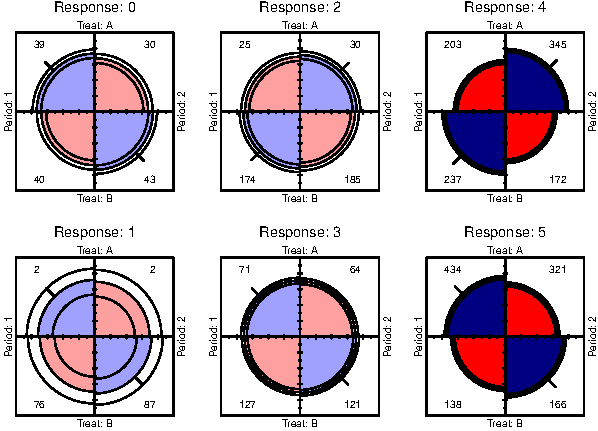
\includegraphics{5_files/figure-pdf/fig-or2-1.pdf}

}

\caption{\label{fig-or2}OR \textasciitilde{} Treat + Period + Response}

\end{figure}

\hypertarget{modelado-1}{%
\section{Modelado}\label{modelado-1}}

La probabilidad de que los alumnos puntúen mejor el subtitulado \(A\)
que el \(B\) frente a que lo puntúen igual o peor se estima que es del
59.95\%. Sin embargo, la distribución por ítems no es uniforme (ver
Tabla~\ref{tbl-improve-question}). Así, hay ítems en que esta
probabilidad sobrepasa el 80\% (Q09, Q05). Sin embargo hay otros en que
no supera el 25\% (Q04, Q16, Q13). La respuesta al ítem Q18 está por
encima de la media (69.82\%). Parece claro que los ítems en los que la
respuesta de los estudiantes es diferente en los dos subtitulados es
porque aprecian diferencias reales entre ellos. Quedaría por dilucidar
si en los ítems en los que no hay diferencia en las respuestas, se debe
a que realmente no las hay o si es que los estudiantes no son capaces de
detectarlas.

La magnitud del efecto del subtitulado sobre las valoraciones es muy
superior a la de los efectos periodo y secuencia (ver
Tabla~\ref{tbl-model-comp}), por lo que podemos realizar
interpretaciones del modelo sin que nos deba preocupar su existencia. En
la Figura~\ref{fig-pred-3} se representan 50 muestras de la esperanza de
la distribución predictiva a posteriori para cada pregunta y nivel de
subtitulado marginalizadas por periodo y estudiante. La primera
conclusión que podemos extraer es que el modelo tiene bastante
incertidumbre sobre los valores de respuesta a cada pregunta no
superando casi nunca el 50\% de probabilidad para todas las preguntas y
niveles de subtitulado. En general se observa en la mayoría de las
preguntas del nivel de subtitulado \(A\) que los alumnos están bastante
seguros de que la respuesta a las preguntas debe ser 4 ó 5, asignando
una muy baja probabilidad a los valores 1, 2, ó 3, pero habiendo
bastante incertidumbre respecto cuál de los dos valores (4 ó 5) asignar.
En el nivel de subtitulado \(B\) la situación es bastante más confusa.
Aunque la opción de respuesta preferida es 4 y las menos preferidas son
la 5 y la 1, hay bastante mezcla entre las opciones de respuesta 2, 3 y
4. En cuanto al análisis individualizado por pregunta podemos extraer
las siguientes conclusiones:

\begin{itemize}
\item
  En las preguntas \(Q04\) y \(Q13\) los estudiantes no aprecian
  defectos en el subtitulado ni diferencias entre un nivel y otro. Son
  valoradas en ambos subtitulados con puntuaciones de 4 y de 5.
\item
  En las preguntas \(Q15\), \(Q16\) y \(Q17\), la opción de respuesta
  más probable es 4 en ambos subtitulados. El modelo asigna una baja
  probabilidad de respuesta a la opción 1 y similares al resto. La
  probabilidad de la opción 5 decrece ligeramente entre subtitulado
  \(A\) y \(B\) y lo contrario ocurre con las opciones 2 y 3.
\item
  Las preguntas \(Q01\), \(Q02\), \(Q03\), \(Q10\), \(Q11\) y \(Q12\)
  son similares a las anteriores. Particularmente en lo referente a que
  la respuesta más probable en el subtitulado \(B\) es 4. En el
  subtitulado \(A\) hay preferencia por 4 y 5. El nivel 5 cae
  acusadamente en el subtitulado \(B\) y en este nivel aumenta
  ligeramente la probabilidad de respuesta 2 y 3.
\item
  Las preguntas \(Q06\), \(Q07\), \(Q14\) y \(Q18\) no son muy
  diferentes de las anteriores. En general el modelo predice mayor
  probabilidad de respuesta para 5 en el subtitulado \(A\) pero este
  valor es con alta probabilidad cercano a cero en el subtitulado \(B\).
  En el subtitulado \(B\) la probabilidad de respuesta 2, 3 ó 4 es
  similar.
\item
  Las preguntas \(Q05\), \(Q08\) y \(Q09\) son las que más diferencias
  entre subtitulados presentan. La respuesta más probable en el
  subtitulado \(A\) es 5 (en \(Q08\) y en \(Q09\) muy parecida a 4). Por
  contra, en el subtitulado \(B\) las respuestas 4 y 5 tienden a cero,
  siendo la más probable la respuesta 2. En \(Q05\) y en \(Q09\) la
  segunda respuesta más probable al subtitulado \(B\) es 1 y 4 en la
  \(Q08\).
\end{itemize}

En definitiva, nuestro modelo predice que los estudiantes están bastante
de acuerdo en que en las preguntas \(Q05\) y \(Q09\) hay una diferencia
de calidad importante entre subtitulados. También están de acuerdo en
que en las preguntas \(Q04\) y \(Q13\) no hay apenas cambio entre los
subtitulados. En las preguntas \(Q15\), \(Q16\) y \(Q17\) hay una gran
confusión en ambos niveles de subtitulado predominando la respuesta 4 y
siendo muy parecidas las respuestas en ambos niveles. En el resto la
confusión se circunscribe al nivel de subtitulado \(B\), ya que en el
nivel \(A\) las opciones 4 y 5 predominan.

\begin{figure}[h]

{\centering 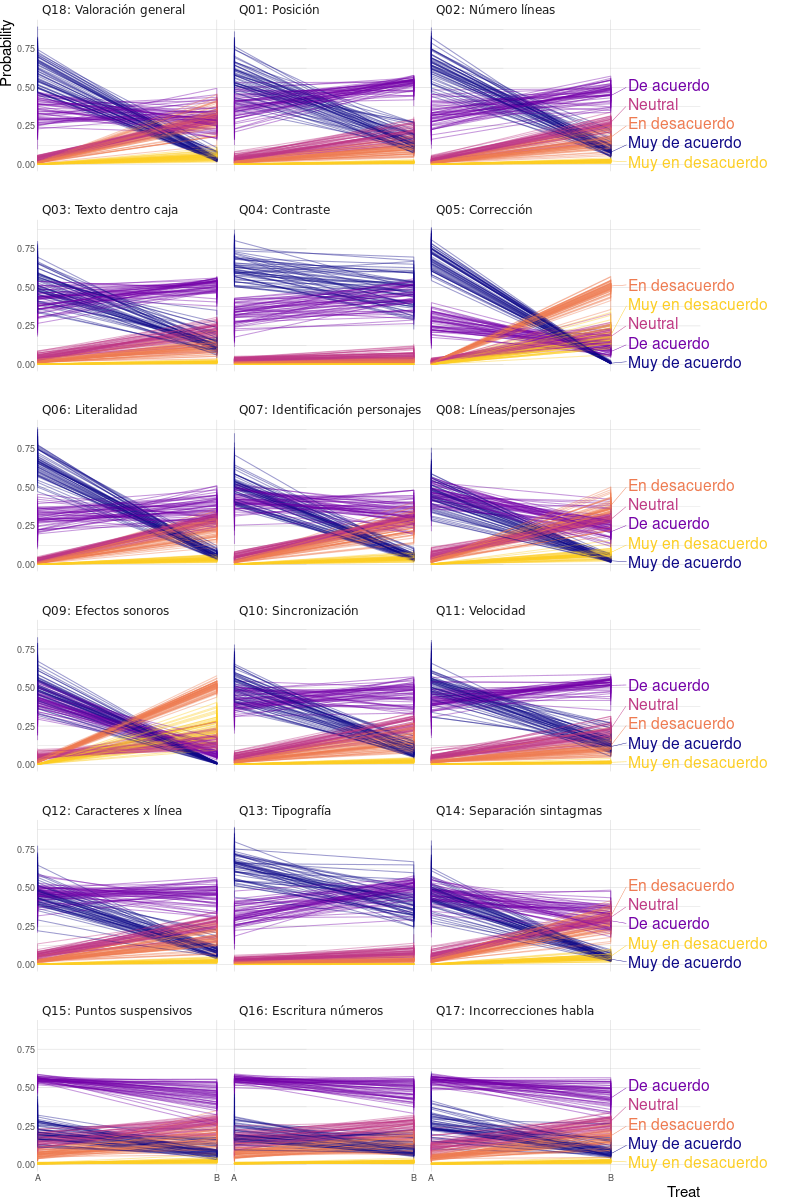
\includegraphics[width=1\textwidth,height=\textheight]{images/bayes-preg.png}

}

\caption{\label{fig-pred-3}Muestreo de la función predictiva a
posteriori por tratamiento y pregunta del modelo Response
\textasciitilde{} Treat * Period + (1 + Treat \textbar{} Subject) + (1 +
Treat \textbar{} Question).}

\end{figure}

\bookmarksetup{startatroot}

\hypertarget{referencias}{%
\chapter*{Referencias}\label{referencias}}
\addcontentsline{toc}{chapter}{Referencias}

\markboth{Referencias}{Referencias}

\printbibliography[heading=none]

\cleardoublepage
\phantomsection
\addcontentsline{toc}{part}{Apéndices}
\appendix

\hypertarget{sec-contrasts}{%
\chapter{Efecto secuencia e interacción tratamiento
vs.~periodo}\label{sec-contrasts}}

Vamos a demostrar que el efecto secuencia es equivalente a la
interacción de los factores tratamiento y periodo.

\hypertarget{preparaciuxf3n}{%
\section{Preparación}\label{preparaciuxf3n}}

Partimos del siguiente conjunto de datos generado aleatoriamente
\footnote{Obsérvese que la variable \texttt{Response} en esta simulación
  es cuantitativa y no ordinal. Se ha realizado de esta forma para poder
  usar un ajuste de mínimos cuadrados en lugar de una regresión ordinal
  para facilitar el cálculo y su interpretación.}: \scriptsize

\begin{Shaded}
\begin{Highlighting}[]
\FunctionTok{set.seed}\NormalTok{(}\DecValTok{100}\NormalTok{)}
\NormalTok{n }\OtherTok{\textless{}{-}} \DecValTok{1000}
\NormalTok{df }\OtherTok{\textless{}{-}} \FunctionTok{data.frame}\NormalTok{(}
    \AttributeTok{Response =} \FunctionTok{rnorm}\NormalTok{(n),}
    \AttributeTok{Treat =} \FunctionTok{as.factor}\NormalTok{(}\FunctionTok{sample}\NormalTok{(}\FunctionTok{c}\NormalTok{(}\StringTok{"A"}\NormalTok{, }\StringTok{"B"}\NormalTok{), n, }\AttributeTok{replace =} \ConstantTok{TRUE}\NormalTok{)),}
    \AttributeTok{Period =} \FunctionTok{as.factor}\NormalTok{(}\FunctionTok{sample}\NormalTok{(}\FunctionTok{c}\NormalTok{(}\DecValTok{1}\NormalTok{, }\DecValTok{2}\NormalTok{), n, }\AttributeTok{replace =} \ConstantTok{TRUE}\NormalTok{))}
\NormalTok{)}

\NormalTok{df}\SpecialCharTok{$}\NormalTok{Seq }\OtherTok{\textless{}{-}} \FunctionTok{as.factor}\NormalTok{(}
    \FunctionTok{ifelse}\NormalTok{(}
\NormalTok{        df}\SpecialCharTok{$}\NormalTok{Period }\SpecialCharTok{==} \DecValTok{1} \SpecialCharTok{\&}\NormalTok{ df}\SpecialCharTok{$}\NormalTok{Treat }\SpecialCharTok{==} \StringTok{"A"} \SpecialCharTok{|}\NormalTok{ df}\SpecialCharTok{$}\NormalTok{Period }\SpecialCharTok{==} \DecValTok{2} \SpecialCharTok{\&}\NormalTok{ df}\SpecialCharTok{$}\NormalTok{Treat }\SpecialCharTok{==} \StringTok{"B"}\NormalTok{,}
        \StringTok{"AB"}\NormalTok{,}
        \StringTok{"BA"}
\NormalTok{    )}
\NormalTok{)}

\FunctionTok{head}\NormalTok{(df, }\DecValTok{10}\NormalTok{)}
\end{Highlighting}
\end{Shaded}

\begin{verbatim}
      Response Treat Period Seq
1  -0.50219235     B      2  AB
2   0.13153117     A      1  AB
3  -0.07891709     A      2  BA
4   0.88678481     A      2  BA
5   0.11697127     A      1  AB
6   0.31863009     A      2  BA
7  -0.58179068     A      2  BA
8   0.71453271     A      1  AB
9  -0.82525943     B      2  AB
10 -0.35986213     B      1  BA
\end{verbatim}

\normalsize

Calculamos las medias por cada nivel de factor y combinaciones de
niveles que utilizaremos luego en la interpretación de los coeficientes
de los modelos

\scriptsize

\begin{Shaded}
\begin{Highlighting}[]
\NormalTok{M }\OtherTok{\textless{}{-}} \FunctionTok{mean}\NormalTok{(df}\SpecialCharTok{$}\NormalTok{Response) }\CommentTok{\# 1 media de respuesta global}

\CommentTok{\# 2 medias de respuesta para tratamientos A y B}
\NormalTok{mTreat }\OtherTok{\textless{}{-}} \FunctionTok{with}\NormalTok{(df, }\FunctionTok{tapply}\NormalTok{(Response, Treat, mean))}

\CommentTok{\# 2 medias de respuesta para periodos 1 y 2}
\NormalTok{mPeriod }\OtherTok{\textless{}{-}} \FunctionTok{with}\NormalTok{(df, }\FunctionTok{tapply}\NormalTok{(Response, Period, mean))}

\CommentTok{\# 2 medias de respuesta para secuencias AB y BA}
\NormalTok{mSeq }\OtherTok{\textless{}{-}} \FunctionTok{with}\NormalTok{(df, }\FunctionTok{tapply}\NormalTok{(Response, Seq, mean))}

\CommentTok{\# 4 medias de respuesta para las cuatro combinaciones de tratamiento y periodo}
\NormalTok{m2 }\OtherTok{\textless{}{-}} \FunctionTok{with}\NormalTok{(df, }\FunctionTok{tapply}\NormalTok{(Response, }\FunctionTok{list}\NormalTok{(Treat, Period), mean))}

\NormalTok{dTreat }\OtherTok{\textless{}{-}} \FunctionTok{diff}\NormalTok{(mTreat) }\CommentTok{\# diferencia de medias entre tratamientos A y B}

\NormalTok{dPeriod }\OtherTok{\textless{}{-}} \FunctionTok{diff}\NormalTok{(mPeriod) }\CommentTok{\# diferencia de medias entre periodos 1 y 2}

\NormalTok{d2 }\OtherTok{\textless{}{-}} \FunctionTok{diff}\NormalTok{(m2) }\CommentTok{\# diferencias entre niveles de tratamiento en cada nivel de periodo}
\end{Highlighting}
\end{Shaded}

\normalsize

\hypertarget{anuxe1lisis-con-un-solo-factor-tratamiento}{%
\section{Análisis con un solo factor
(tratamiento)}\label{anuxe1lisis-con-un-solo-factor-tratamiento}}

\scriptsize

\begin{Shaded}
\begin{Highlighting}[]
\NormalTok{l1 }\OtherTok{\textless{}{-}} \FunctionTok{lm}\NormalTok{(Response }\SpecialCharTok{\textasciitilde{}}\NormalTok{ Treat, df)}
\FunctionTok{data.frame}\NormalTok{(}\FunctionTok{t}\NormalTok{(}\FunctionTok{coef}\NormalTok{(l1))) }\SpecialCharTok{\%\textgreater{}\%} \FunctionTok{gt}\NormalTok{()}
\end{Highlighting}
\end{Shaded}

\hypertarget{tbl-l1}{}
\begin{longtable}{rr}
\caption{\label{tbl-l1}Ajuste del modelo Response \textasciitilde{} Treat con contrasts
treatment. }\tabularnewline

\toprule
X.Intercept. & TreatB \\ 
\midrule
0.03624217 & -0.03966751 \\ 
\bottomrule
\end{longtable}

\normalsize

Vemos que el intercepto es la media de la respuesta en el nivel de
tratamiento \(A\):

\scriptsize

\begin{Shaded}
\begin{Highlighting}[]
\NormalTok{mTreat[}\DecValTok{1}\NormalTok{]}
\end{Highlighting}
\end{Shaded}

\begin{verbatim}
         A 
0.03624217 
\end{verbatim}

\normalsize

Que la pendiente (parámetro \(TreatB\)) es la diferencia entre las
medias tratamientos:

\scriptsize

\begin{Shaded}
\begin{Highlighting}[]
\NormalTok{dTreat}
\end{Highlighting}
\end{Shaded}

\begin{verbatim}
          B 
-0.03966751 
\end{verbatim}

\normalsize

Por ello, para conocer el efecto del tratamiento en el nivel \(B\) hay
que sumar intercepto y pendiente:

\scriptsize

\begin{Shaded}
\begin{Highlighting}[]
\FunctionTok{coef}\NormalTok{(l1)[[}\DecValTok{1}\NormalTok{]] }\SpecialCharTok{+} \FunctionTok{coef}\NormalTok{(l1)[[}\DecValTok{2}\NormalTok{]] }\SpecialCharTok{{-}}\NormalTok{ mTreat[[}\DecValTok{2}\NormalTok{]]}
\end{Highlighting}
\end{Shaded}

\begin{verbatim}
[1] 1.214306e-16
\end{verbatim}

\normalsize

Esto es así ya que por defecto R utiliza el contraste conocido como
\texttt{codificación\ de\ tratamiento}:

\scriptsize

\begin{Shaded}
\begin{Highlighting}[]
\FunctionTok{contr.treatment}\NormalTok{(}\DecValTok{2}\NormalTok{)}
\end{Highlighting}
\end{Shaded}

\begin{verbatim}
  2
1 0
2 1
\end{verbatim}

\normalsize

Podemos ver la matriz ampliada añadiendo el intercepto, que siempre será
una columna de 1's:

\scriptsize

\begin{Shaded}
\begin{Highlighting}[]
\FunctionTok{model.matrix}\NormalTok{(}\SpecialCharTok{\textasciitilde{}}\NormalTok{Treat, }\FunctionTok{expand.grid}\NormalTok{(}\AttributeTok{Treat =} \FunctionTok{c}\NormalTok{(}\StringTok{"A"}\NormalTok{, }\StringTok{"B"}\NormalTok{)))}
\end{Highlighting}
\end{Shaded}

\begin{verbatim}
  (Intercept) TreatB
1           1      0
2           1      1
attr(,"assign")
[1] 0 1
attr(,"contrasts")
attr(,"contrasts")$Treat
[1] "contr.treatment"
\end{verbatim}

\normalsize

Cada fila representa el nivel del tratamiento (fila 1 nivel \(A\) y fila
2 nivel \(B\)) y las columnas representan los parámetros del modelo. Los
valores son los niveles de tratamiento (0 ó 1). Para obtener el
significado de cada parámetro, multiplicamos el valor del contraste por
el parámetro. Así:

\begin{itemize}
\tightlist
\item
  De la primera fila obtenemos que el efecto del tratamiento \(A\) es el
  intercepto: \(A = 1 \cdot Intercept + 0 \cdot TreatB\).
\item
  De la segunda fila obtenemos que el valor del parámetro \(TreatB\) es
  la diferencia de los niveles de tratamiento.
  \(B = 1 \cdot Intercept + 1 \cdot TreatB \Rightarrow TreatB = B - Intercept\).
\end{itemize}

Esto quiere decir que existe una variable para codificar el efecto
tratamiento, y esta variable tiene el valor 0 para el nivel \(A\) por
ser el de referencia y 1 para el nivel \(B\). La pendiente se codifica
como la diferencia del efecto de los dos niveles (\(B - A\)).

\hypertarget{anuxe1lisis-con-un-dos-factores-tratamiento-y-periodo}{%
\section{Análisis con un dos factores (tratamiento y
periodo)}\label{anuxe1lisis-con-un-dos-factores-tratamiento-y-periodo}}

\scriptsize

\begin{Shaded}
\begin{Highlighting}[]
\NormalTok{l2 }\OtherTok{\textless{}{-}} \FunctionTok{lm}\NormalTok{(Response }\SpecialCharTok{\textasciitilde{}}\NormalTok{ Treat }\SpecialCharTok{*}\NormalTok{ Period, df)}
\FunctionTok{data.frame}\NormalTok{(}\FunctionTok{t}\NormalTok{(}\FunctionTok{coef}\NormalTok{(l2))) }\SpecialCharTok{\%\textgreater{}\%} \FunctionTok{gt}\NormalTok{()}
\end{Highlighting}
\end{Shaded}

\hypertarget{tbl-l2}{}
\begin{longtable}{rrrr}
\caption{\label{tbl-l2}Ajuste del modelo Response \textasciitilde{} Treat * Period con
contrasts treatment. }\tabularnewline

\toprule
X.Intercept. & TreatB & Period2 & TreatB.Period2 \\ 
\midrule
0.04138614 & -0.1076137 & -0.01125933 & 0.1343517 \\ 
\bottomrule
\end{longtable}

\normalsize

Vemos que el intercepto es la media del tratamiento \(A\) en el periodo
\(1\) por ser estos los valores que R usa como referencia \footnote{R
  utiliza como valor de referencia el nivel más bajo de factor.}:

\scriptsize

\begin{Shaded}
\begin{Highlighting}[]
\NormalTok{m2[}\StringTok{"A"}\NormalTok{, }\StringTok{"1"}\NormalTok{]}
\end{Highlighting}
\end{Shaded}

\begin{verbatim}
[1] 0.04138614
\end{verbatim}

\normalsize

El parámetro \(TreatB\) es la diferencia de medias entre los
tratamientos en el periodo \(1\):

\scriptsize

\begin{Shaded}
\begin{Highlighting}[]
\NormalTok{m2[}\StringTok{"B"}\NormalTok{, }\StringTok{"1"}\NormalTok{] }\SpecialCharTok{{-}}\NormalTok{ m2[}\StringTok{"A"}\NormalTok{, }\StringTok{"1"}\NormalTok{]}
\end{Highlighting}
\end{Shaded}

\begin{verbatim}
[1] -0.1076137
\end{verbatim}

\normalsize

El parámetro \(Period2\) es la diferencia de medias entre los periodos
en el nivel de tratamiento \(A\):

\scriptsize

\begin{Shaded}
\begin{Highlighting}[]
\NormalTok{m2[}\StringTok{"A"}\NormalTok{, }\StringTok{"2"}\NormalTok{] }\SpecialCharTok{{-}}\NormalTok{ m2[}\StringTok{"A"}\NormalTok{, }\StringTok{"1"}\NormalTok{]}
\end{Highlighting}
\end{Shaded}

\begin{verbatim}
[1] -0.01125933
\end{verbatim}

\normalsize

Finalmente, \(TreatB:Period2\) es la diferencia entre el segundo periodo
y el primero del nivel de tratamiento \(B\) menos la diferencia entre
periodos del nivel de tratamiento \(A\):

\scriptsize

\begin{Shaded}
\begin{Highlighting}[]
\NormalTok{m2[}\StringTok{"B"}\NormalTok{, }\StringTok{"2"}\NormalTok{] }\SpecialCharTok{{-}}\NormalTok{ m2[}\StringTok{"B"}\NormalTok{, }\StringTok{"1"}\NormalTok{] }\SpecialCharTok{{-}}\NormalTok{ (m2[}\StringTok{"A"}\NormalTok{, }\StringTok{"2"}\NormalTok{] }\SpecialCharTok{{-}}\NormalTok{ m2[}\StringTok{"A"}\NormalTok{, }\StringTok{"1"}\NormalTok{])}
\end{Highlighting}
\end{Shaded}

\begin{verbatim}
[1] 0.1343517
\end{verbatim}

\normalsize

La matriz de contraste nos permite razonar por qué esto es así:

\scriptsize

\begin{Shaded}
\begin{Highlighting}[]
\FunctionTok{model.matrix}\NormalTok{(}\SpecialCharTok{\textasciitilde{}}\NormalTok{ Treat }\SpecialCharTok{*}\NormalTok{ Period, }\FunctionTok{expand.grid}\NormalTok{(}\AttributeTok{Treat =} \FunctionTok{c}\NormalTok{(}\StringTok{"A"}\NormalTok{, }\StringTok{"B"}\NormalTok{), }\AttributeTok{Period =} \FunctionTok{c}\NormalTok{(}\StringTok{"1"}\NormalTok{, }\StringTok{"2"}\NormalTok{)))}
\end{Highlighting}
\end{Shaded}

\begin{verbatim}
  (Intercept) TreatB Period2 TreatB:Period2
1           1      0       0              0
2           1      1       0              0
3           1      0       1              0
4           1      1       1              1
attr(,"assign")
[1] 0 1 2 3
attr(,"contrasts")
attr(,"contrasts")$Treat
[1] "contr.treatment"

attr(,"contrasts")$Period
[1] "contr.treatment"
\end{verbatim}

\normalsize

\begin{itemize}
\tightlist
\item
  La primera fila es el intercepto y corresponde con el tratamiento
  \(A\) y el periodo 1.
\item
  La segunda fila es el efecto del tratamiento \(B\) en el periodo 1 y
  se calcula con la suma del intercepto y el parámetro \(TreatB\). Luego
  \(TreatB\) es la diferencia del efecto de los tratamientos en el
  periodo 1.
\item
  Análogamente con la tercera fila concluimos que \(Period2\) es la
  deferencia entre periodos para el tratamiento \(A\).
\item
  Finalmente, la cuarta fila, es el tratamiento \(B\) en el periodo 2 y,
  por lo tanto, \(Treat2:Period2\) es la diferencia el nivel \(B\) de
  tratamiento y el periodo 2 y el nivel de tratamiento \(A\) en el
  periodo 1, menos la diferencia de niveles de tratamiento para el
  periodo 1 y menos la diferencia de periodos para el tratamiento \(A\).
\end{itemize}

Obsérvese que antes hemos calculado de forma diferente
\(TreatB:Period2\). Podemos aplicar la fórmula anterior y comprobar que
produce el mismo resultado:

\scriptsize

\begin{Shaded}
\begin{Highlighting}[]
\NormalTok{m2[}\StringTok{"B"}\NormalTok{, }\StringTok{"2"}\NormalTok{] }\SpecialCharTok{{-}}\NormalTok{ m2[}\StringTok{"A"}\NormalTok{, }\StringTok{"1"}\NormalTok{] }\SpecialCharTok{{-}}\NormalTok{ (m2[}\StringTok{"B"}\NormalTok{, }\StringTok{"1"}\NormalTok{] }\SpecialCharTok{{-}}\NormalTok{ m2[}\StringTok{"A"}\NormalTok{, }\StringTok{"1"}\NormalTok{]) }\SpecialCharTok{{-}}\NormalTok{ (m2[}\StringTok{"A"}\NormalTok{, }\StringTok{"2"}\NormalTok{] }\SpecialCharTok{{-}}\NormalTok{ m2[}\StringTok{"A"}\NormalTok{, }\StringTok{"1"}\NormalTok{])}
\end{Highlighting}
\end{Shaded}

\begin{verbatim}
[1] 0.1343517
\end{verbatim}

\normalsize

\hypertarget{factor-secuencia}{%
\section{Factor secuencia}\label{factor-secuencia}}

Vamos a incorporar la secuencia como factor para ver si es equivalente a
la interacción entre periodo y tratamiento. En caso de serlo los
coeficientes del modelo ajustado deberían coincidir. Sin embargo vemos
que los modelos l2 (Tabla~\ref{tbl-l2}) y l3 (Tabla~\ref{tbl-l3}) tienen
distintos coeficientes.

\scriptsize

\begin{Shaded}
\begin{Highlighting}[]
\NormalTok{l3 }\OtherTok{\textless{}{-}} \FunctionTok{lm}\NormalTok{(Response }\SpecialCharTok{\textasciitilde{}}\NormalTok{ Treat }\SpecialCharTok{+}\NormalTok{ Period }\SpecialCharTok{+}\NormalTok{ Seq, df)}
\FunctionTok{data.frame}\NormalTok{(}\FunctionTok{t}\NormalTok{(}\FunctionTok{coef}\NormalTok{(l3))) }\SpecialCharTok{\%\textgreater{}\%} \FunctionTok{gt}\NormalTok{()}
\end{Highlighting}
\end{Shaded}

\hypertarget{tbl-l3}{}
\begin{longtable}{rrrr}
\caption{\label{tbl-l3}Ajuste del modelo Response \textasciitilde{} Treat + Period + Seq con
contrasts treatment. }\tabularnewline

\toprule
X.Intercept. & TreatB & Period2 & SeqBA \\ 
\midrule
0.04138614 & -0.04043786 & 0.05591654 & -0.06717587 \\ 
\bottomrule
\end{longtable}

\normalsize

Los coeficientes no coinciden debido a que estamos usando el contraste
con \texttt{codificación\ de\ tratamientos}. Pero si cambiamos a
\texttt{codificación\ de\ sumas}:

\scriptsize

\begin{Shaded}
\begin{Highlighting}[]
\FunctionTok{options}\NormalTok{(}\AttributeTok{contrasts =} \FunctionTok{rep}\NormalTok{(}\StringTok{"contr.sum"}\NormalTok{, }\DecValTok{2}\NormalTok{))}
\end{Highlighting}
\end{Shaded}

\normalsize

Y volvemos a ajustar los modelos que ya usarán el
\texttt{contraste\ suma}, podemos comprobar que ahora tienen los mismos
coeficientes y el coeficiente \(Seq1\) del modelo que incorpora el
efecto secuencia (Tabla~\ref{tbl-l4}) es igual que el coeficiente
\(Treat1:Period1\) del modelo que incorpora la interacción entre
tratamiento y periodo (Tabla~\ref{tbl-l5}). Obsérvese que los nombres de
los coeficientes han cambiado respecto al
\texttt{contraste\ de\ tratamiento}. Esto sucede porque la
interpretación de los coeficientes varía como se explica a continuación.

\scriptsize

\begin{Shaded}
\begin{Highlighting}[]
\NormalTok{l4 }\OtherTok{\textless{}{-}} \FunctionTok{lm}\NormalTok{(Response }\SpecialCharTok{\textasciitilde{}}\NormalTok{ Treat }\SpecialCharTok{+}\NormalTok{ Period }\SpecialCharTok{+}\NormalTok{ Seq, df)}
\FunctionTok{data.frame}\NormalTok{(}\FunctionTok{t}\NormalTok{(}\FunctionTok{coef}\NormalTok{(l4))) }\SpecialCharTok{\%\textgreater{}\%} \FunctionTok{gt}\NormalTok{()}
\end{Highlighting}
\end{Shaded}

\hypertarget{tbl-l4}{}
\begin{longtable}{rrrr}
\caption{\label{tbl-l4}Ajuste del modelo Response \textasciitilde{} Treat + Period + Seq con
contrasts sum. }\tabularnewline

\toprule
X.Intercept. & Treat1 & Period1 & Seq1 \\ 
\midrule
0.01553755 & 0.02021893 & -0.02795827 & 0.03358794 \\ 
\bottomrule
\end{longtable}

\normalsize

\scriptsize

\begin{Shaded}
\begin{Highlighting}[]
\NormalTok{l5 }\OtherTok{\textless{}{-}} \FunctionTok{lm}\NormalTok{(Response }\SpecialCharTok{\textasciitilde{}}\NormalTok{ Treat }\SpecialCharTok{*}\NormalTok{ Period, df)}
\FunctionTok{data.frame}\NormalTok{(}\FunctionTok{t}\NormalTok{(}\FunctionTok{coef}\NormalTok{(l5))) }\SpecialCharTok{\%\textgreater{}\%} \FunctionTok{gt}\NormalTok{()}
\end{Highlighting}
\end{Shaded}

\hypertarget{tbl-l5}{}
\begin{longtable}{rrrr}
\caption{\label{tbl-l5}Ajuste del modelo Response \textasciitilde{} Treat * Period con
contrasts sum. }\tabularnewline

\toprule
X.Intercept. & Treat1 & Period1 & Treat1.Period1 \\ 
\midrule
0.01553755 & 0.02021893 & -0.02795827 & 0.03358794 \\ 
\bottomrule
\end{longtable}

\normalsize

La interpretación de los coeficientes es diferente. Para explicarlo,
mostramos la matriz de contraste:

\scriptsize

\begin{Shaded}
\begin{Highlighting}[]
\FunctionTok{model.matrix}\NormalTok{(}\SpecialCharTok{\textasciitilde{}}\NormalTok{ Treat }\SpecialCharTok{*}\NormalTok{ Period, }\FunctionTok{expand.grid}\NormalTok{(}\AttributeTok{Treat =} \FunctionTok{c}\NormalTok{(}\StringTok{"A"}\NormalTok{, }\StringTok{"B"}\NormalTok{), }\AttributeTok{Period =} \FunctionTok{c}\NormalTok{(}\StringTok{"1"}\NormalTok{, }\StringTok{"2"}\NormalTok{)))}
\end{Highlighting}
\end{Shaded}

\begin{verbatim}
  (Intercept) Treat1 Period1 Treat1:Period1
1           1      1       1              1
2           1     -1       1             -1
3           1      1      -1             -1
4           1     -1      -1              1
attr(,"assign")
[1] 0 1 2 3
attr(,"contrasts")
attr(,"contrasts")$Treat
[1] "contr.sum"

attr(,"contrasts")$Period
[1] "contr.sum"
\end{verbatim}

\normalsize

Vemos que ahora los niveles son 1 y -1 \footnote{El nivel de referencia
  del factor tendrá valor 1 y el otro -1. Por ejemplo, en la variable
  \texttt{Treat}, \(A\) tendrá +1 y \(B\) tendrá valor -1.} en vez de 0
y 1 que se utilizan en el contraste de tratamiento. La interpretación es
la siguiente:

\begin{itemize}
\tightlist
\item
  El interceptor es la media de la media de cada uno de los niveles de
  factor. ¿Por qué?. El interceptor es el valor de la variable de
  respuesta cuando cuando todas las variables explicativas valen 0. Esto
  sucede en la media de la variable de respuesta ya que cero es el valor
  que está en la mitad de +1 y -1. Podemos comprobar que la media global
  coincide con el interceptor del modelo l4 (Tabla~\ref{tbl-l4}):
\end{itemize}

\scriptsize

\begin{Shaded}
\begin{Highlighting}[]
\FunctionTok{mean}\NormalTok{(m2)}
\end{Highlighting}
\end{Shaded}

\begin{verbatim}
[1] 0.01553755
\end{verbatim}

\normalsize

\begin{itemize}
\tightlist
\item
  El coeficiente \(Treat1\) es la mitad la diferencia de la media entre
  niveles de tratamiento (\(TreatA-TreatB\)). La media de cada
  tratamiento se calcula como la media del tratamiento en cada periodo.
\end{itemize}

\scriptsize

\begin{Shaded}
\begin{Highlighting}[]
\SpecialCharTok{{-}}\FunctionTok{diff}\NormalTok{(}\FunctionTok{apply}\NormalTok{(m2, }\DecValTok{1}\NormalTok{, mean)) }\SpecialCharTok{/} \DecValTok{2}
\end{Highlighting}
\end{Shaded}

\begin{verbatim}
         B 
0.02021893 
\end{verbatim}

\normalsize

Otra forma de entender el coeficiente \(Treat1\) es como la cuarta parte
de la diferencia de los efectos de los tratamientos en cada periodo.

\scriptsize

\begin{Shaded}
\begin{Highlighting}[]
\NormalTok{(m2[}\StringTok{"A"}\NormalTok{, }\StringTok{"1"}\NormalTok{] }\SpecialCharTok{+}\NormalTok{ m2[}\StringTok{"A"}\NormalTok{, }\StringTok{"2"}\NormalTok{] }\SpecialCharTok{{-}}\NormalTok{ (m2[}\StringTok{"B"}\NormalTok{, }\StringTok{"1"}\NormalTok{] }\SpecialCharTok{+}\NormalTok{ m2[}\StringTok{"B"}\NormalTok{, }\StringTok{"2"}\NormalTok{])) }\SpecialCharTok{/} \DecValTok{4}
\end{Highlighting}
\end{Shaded}

\begin{verbatim}
[1] 0.02021893
\end{verbatim}

\normalsize

\begin{itemize}
\tightlist
\item
  El coeficiente \(Period1\) es la mitad la diferencia de la media entre
  periodos(\(Period1 - Period2\)). La media entre periodos se calcula
  como la media del periodo para cada tratamiento.
\end{itemize}

\scriptsize

\begin{Shaded}
\begin{Highlighting}[]
\SpecialCharTok{{-}}\FunctionTok{diff}\NormalTok{(}\FunctionTok{apply}\NormalTok{(m2, }\DecValTok{2}\NormalTok{, mean)) }\SpecialCharTok{/} \DecValTok{2}
\end{Highlighting}
\end{Shaded}

\begin{verbatim}
          2 
-0.02795827 
\end{verbatim}

\normalsize

Otra forma de entender el coeficiente \(Period1\) es como la cuarta
parte de la diferencia de los efectos del periodo en cada tratamiento.

\scriptsize

\begin{Shaded}
\begin{Highlighting}[]
\NormalTok{(m2[}\StringTok{"A"}\NormalTok{, }\StringTok{"1"}\NormalTok{] }\SpecialCharTok{+}\NormalTok{ m2[}\StringTok{"B"}\NormalTok{, }\StringTok{"1"}\NormalTok{] }\SpecialCharTok{{-}}\NormalTok{ (m2[}\StringTok{"A"}\NormalTok{, }\StringTok{"2"}\NormalTok{] }\SpecialCharTok{+}\NormalTok{ m2[}\StringTok{"B"}\NormalTok{, }\StringTok{"2"}\NormalTok{])) }\SpecialCharTok{/} \DecValTok{4}
\end{Highlighting}
\end{Shaded}

\begin{verbatim}
[1] -0.02795827
\end{verbatim}

\normalsize

\begin{itemize}
\tightlist
\item
  El coeficiente \(Treat1:Period1\) es el coeficiente \(Treat1\) menos
  la mitad de la diferencia de la media entre tratamientos para el
  periodo 2 (\(TreatA-TreatB\)):
\end{itemize}

\scriptsize

\begin{Shaded}
\begin{Highlighting}[]
\SpecialCharTok{{-}}\FunctionTok{diff}\NormalTok{(}\FunctionTok{apply}\NormalTok{(m2, }\DecValTok{1}\NormalTok{, mean)) }\SpecialCharTok{/} \DecValTok{2} \SpecialCharTok{+} \FunctionTok{diff}\NormalTok{(m2[, }\StringTok{"2"}\NormalTok{]) }\SpecialCharTok{/} \DecValTok{2}
\end{Highlighting}
\end{Shaded}

\begin{verbatim}
         B 
0.03358794 
\end{verbatim}

\begin{Shaded}
\begin{Highlighting}[]
\FunctionTok{coef}\NormalTok{(l5)[}\DecValTok{2}\NormalTok{] }\SpecialCharTok{+} \FunctionTok{diff}\NormalTok{(m2[, }\StringTok{"2"}\NormalTok{]) }\SpecialCharTok{/} \DecValTok{2}
\end{Highlighting}
\end{Shaded}

\begin{verbatim}
    Treat1 
0.03358794 
\end{verbatim}

\normalsize

El coeficiente \(Treat1:Period1\) también se puede calcular como
\(Period1\) menos la mitad de la diferencia de la media entre periodos
para el para el tratamiento \(B\) (\(Period1-Period2\)):

\scriptsize

\begin{Shaded}
\begin{Highlighting}[]
\SpecialCharTok{{-}}\FunctionTok{diff}\NormalTok{(}\FunctionTok{apply}\NormalTok{(m2, }\DecValTok{2}\NormalTok{, mean)) }\SpecialCharTok{/} \DecValTok{2} \SpecialCharTok{+} \FunctionTok{diff}\NormalTok{(m2[}\StringTok{"B"}\NormalTok{, ]) }\SpecialCharTok{/} \DecValTok{2}
\end{Highlighting}
\end{Shaded}

\begin{verbatim}
         2 
0.03358794 
\end{verbatim}

\begin{Shaded}
\begin{Highlighting}[]
\FunctionTok{coef}\NormalTok{(l5)[}\DecValTok{3}\NormalTok{] }\SpecialCharTok{+} \FunctionTok{diff}\NormalTok{(m2[}\StringTok{"B"}\NormalTok{, ]) }\SpecialCharTok{/} \DecValTok{2}
\end{Highlighting}
\end{Shaded}

\begin{verbatim}
   Period1 
0.03358794 
\end{verbatim}

\normalsize

Un tercera forma de interpretar el coeficiente \(Treat1:Period1\) es
como la cuarta parte de la suma de la diferencia cruzada del efecto de
cada tratamiento en cada periodo:

\scriptsize

\begin{Shaded}
\begin{Highlighting}[]
\NormalTok{(m2[}\StringTok{"A"}\NormalTok{, }\StringTok{"1"}\NormalTok{] }\SpecialCharTok{{-}}\NormalTok{ m2[}\StringTok{"A"}\NormalTok{, }\StringTok{"2"}\NormalTok{] }\SpecialCharTok{+}\NormalTok{ m2[}\StringTok{"B"}\NormalTok{, }\StringTok{"2"}\NormalTok{] }\SpecialCharTok{{-}}\NormalTok{ m2[}\StringTok{"B"}\NormalTok{, }\StringTok{"1"}\NormalTok{]) }\SpecialCharTok{/} \DecValTok{4}
\end{Highlighting}
\end{Shaded}

\begin{verbatim}
[1] 0.03358794
\end{verbatim}

\normalsize

O reorganizando los términos de otra forma, sería la cuarta parte de la
suma de la diferencia cruzada del efecto de cada periodo en cada
tratamiento:

\scriptsize

\begin{Shaded}
\begin{Highlighting}[]
\NormalTok{(m2[}\StringTok{"B"}\NormalTok{, }\StringTok{"2"}\NormalTok{] }\SpecialCharTok{{-}}\NormalTok{ m2[}\StringTok{"A"}\NormalTok{, }\StringTok{"2"}\NormalTok{] }\SpecialCharTok{+}\NormalTok{ m2[}\StringTok{"A"}\NormalTok{, }\StringTok{"1"}\NormalTok{] }\SpecialCharTok{{-}}\NormalTok{ m2[}\StringTok{"B"}\NormalTok{, }\StringTok{"1"}\NormalTok{]) }\SpecialCharTok{/} \DecValTok{4}
\end{Highlighting}
\end{Shaded}

\begin{verbatim}
[1] 0.03358794
\end{verbatim}

\normalsize

\begin{itemize}
\tightlist
\item
  Podemos obtener el coeficiente \(TreatB\) del modelo \(l2\)
  (Tabla~\ref{tbl-l2}) como \(-2 \cdot (Treat1 + Treat1:Period1)\):
\end{itemize}

\scriptsize

\begin{Shaded}
\begin{Highlighting}[]
\SpecialCharTok{{-}}\DecValTok{2} \SpecialCharTok{*}\NormalTok{ (}\FunctionTok{coef}\NormalTok{(l5)[}\StringTok{"Treat1"}\NormalTok{] }\SpecialCharTok{+} \FunctionTok{coef}\NormalTok{(l5)[}\StringTok{"Treat1:Period1"}\NormalTok{])}
\end{Highlighting}
\end{Shaded}

\begin{verbatim}
    Treat1 
-0.1076137 
\end{verbatim}

\normalsize

\begin{itemize}
\tightlist
\item
  Análogamente el coeficiente \(Period2\) del modelo \(l2\)
  (Tabla~\ref{tbl-l2}) se obtiene
  \(-2 \cdot (Period1 + Treat1:Period1)\):
\end{itemize}

\scriptsize

\begin{Shaded}
\begin{Highlighting}[]
\SpecialCharTok{{-}}\DecValTok{2} \SpecialCharTok{*}\NormalTok{ (}\FunctionTok{coef}\NormalTok{(l5)[}\StringTok{"Period1"}\NormalTok{] }\SpecialCharTok{+} \FunctionTok{coef}\NormalTok{(l5)[}\StringTok{"Treat1:Period1"}\NormalTok{])}
\end{Highlighting}
\end{Shaded}

\begin{verbatim}
    Period1 
-0.01125933 
\end{verbatim}

\normalsize

\begin{itemize}
\tightlist
\item
  El coeficiente \(TreatB:Period2\) se obtiene como
  \(4 \cdot Treat1:Period1\):
\end{itemize}

\scriptsize

\begin{Shaded}
\begin{Highlighting}[]
\DecValTok{4} \SpecialCharTok{*}\NormalTok{ (}\FunctionTok{coef}\NormalTok{(l5)[}\StringTok{"Treat1:Period1"}\NormalTok{])}
\end{Highlighting}
\end{Shaded}

\begin{verbatim}
Treat1:Period1 
     0.1343517 
\end{verbatim}

\normalsize

\hypertarget{resumen-de-modelos-y-equivalencias-de-paruxe1metros}{%
\section{Resumen de modelos y equivalencias de
parámetros}\label{resumen-de-modelos-y-equivalencias-de-paruxe1metros}}

En la Tabla \ref{tbl-contrasts-compare} se muestran las equivalencias de
los coeficientes de cada modelo. Todas las filas de la misma columna
corresponden a un determinado nivel para cada factor y la fórmula
mostrada es el modelo resultante teniendo en cuenta que:

\begin{itemize}
\item
  En el contraste \texttt{treatment} se utiliza como referencia el
  primer nivel de cada factor, que corresponderá con el intercepto; los
  coeficientes se denominan \((Intercept)\), \(TreatB\), \(Period2\) y
  \(SeqBA\) y son la diferencia del nivel que representa cada
  coeficiente con el intercepto; y los valores de cada nivel de factor
  son: \(TreatA = 0\), \(TreatB = 1\), \(Period1 = 0\), \(Period2 = 1\),
  \(SeqAB = 0\), \(SeqBA = 1\).
\item
  En el contraste \texttt{sum}, el intercepto es el valor medio y se
  excluye elcoeficiente del último nivel que se calcula como la suma del
  resto de niveles con signo opuesto \footnote{Como en este caso solo
    hay dos niveles en cada factor, el valor del segundo nivel será
    simplemente el opuesto del primer nivel.}; los coeficientes se
  denominan \((Intercept)\), \(Treat1\), \(Period1\) y \(Seq1\); y los
  valores de cada nivel de factor son:\(TreatA = 1\), \(TreatB = -1\),
  \(Period1 = 1\), \(Period2 = -1\), \(SeqAB = 1\), \(SeqBA = -1\).
\end{itemize}

\begin{table}[H]
\caption{\label{tbl-contrasts-compare}Equivalencia entre coeficientes y modelos.}\tabularnewline
\tiny
\begin{adjustwidth}{-3.5cm}{}
% Please add the following required packages to your document preamble:
\begin{tabular}{@{}|c|l|llll|@{}}
\toprule
\multicolumn{1}{|l|}{} &
  \multicolumn{1}{c|}{} &
  \multicolumn{4}{c|}{\textbf{Factor Levels}} \\ \cmidrule(l){3-6} 
\multicolumn{1}{|l|}{\multirow{-2}{*}{\textbf{Contrast}}} &
  \multicolumn{1}{c|}{\multirow{-2}{*}{\textbf{Model}}} &
  \multicolumn{1}{c|}{{\color[HTML]{9A0000} \textbf{\begin{tabular}[c]{@{}c@{}}TreatA\\ Period1\\ SeqAB\end{tabular}}}} &
  \multicolumn{1}{c|}{{\color[HTML]{3531FF} \textbf{\begin{tabular}[c]{@{}c@{}}TreatA\\ Period2\\ SeqBA\end{tabular}}}} &
  \multicolumn{1}{c|}{{\color[HTML]{646809} \textbf{\begin{tabular}[c]{@{}c@{}}TreatB\\ Period1\\ SeqBA\end{tabular}}}} &
  \multicolumn{1}{c|}{{\color[HTML]{986536} \textbf{\begin{tabular}[c]{@{}c@{}}TreatB\\ Period2\\ SeqAB\end{tabular}}}} \\ \midrule
 &
  $R \! = \! \beta_0 \! +\!  \beta_1Treat \! +\!  \beta_2Period \! +\!  \beta_3Treat\!:\!Period$ &
  \multicolumn{1}{l|}{{\color[HTML]{9A0000} $R \! = \! \beta_0$}} &
  \multicolumn{1}{l|}{{\color[HTML]{3531FF} $R \! = \! \beta_0 \! +\!  \beta_2$}} &
  \multicolumn{1}{l|}{{\color[HTML]{646809} $R \! = \! \beta_0 \! +\!  \beta_1$}} &
  {\color[HTML]{986536} $R \! = \! \beta_0 \! +\!  \beta_1 \! +\!  \beta_2 \! +\!  \beta_3$} \\ \cmidrule(l){2-6} 
\multirow{-2}{*}{\textbf{Treatment}} &
  $R \! = \! \beta_0 \! +\!  \beta_1Treat \! +\!  \beta_2Period \! +\!  \beta_3Seq$ &
  \multicolumn{1}{l|}{{\color[HTML]{9A0000} $R \! = \! \beta_0$}} &
  \multicolumn{1}{l|}{{\color[HTML]{3531FF} $R \! = \! \beta_0 \! +\!  \beta_2 \! +\!  \beta_3$}} &
  \multicolumn{1}{l|}{{\color[HTML]{646809} $R \! = \! \beta_0 \! +\!  \beta_1 \! +\!  \beta_3$}} &
  {\color[HTML]{986536} $R \! = \! \beta_0 \! +\!  \beta_1 \! +\!  \beta_2$} \\ \midrule
 &
  $R \! = \! \beta_0 \! +\!  \beta_1Treat \! +\!  \beta_2Period \! +\!  \beta_3Treat\!:\!Period$ &
  \multicolumn{1}{l|}{{\color[HTML]{9A0000} $R \! = \! \beta_0 \! +\!  \beta_1 \! +\!  \beta_2 \! +\!  \beta_3$}} &
  \multicolumn{1}{l|}{{\color[HTML]{3531FF} $R \! = \! \beta_0 \! +\!  \beta_1 \! -\! \beta_2 \! -\! \beta_3$}} &
  \multicolumn{1}{l|}{{\color[HTML]{646809} $R \! = \! \beta_0 \! -\! \beta_1 \! +\!  \beta_2 \! -\! \beta_3$}} &
  {\color[HTML]{986536} $R \! = \! \beta_0 \! -\! \beta_1 \! -\! \beta_2 \! +\!  \beta_3$} \\ \cmidrule(l){2-6} 
\multirow{-2}{*}{\textbf{Sum}} &
  $R \! = \! \beta_0 \! +\!  \beta_1Treat \! +\!  \beta_2Period \! +\!  \beta_3Seq$ &
  \multicolumn{1}{l|}{{\color[HTML]{9A0000} $R \! = \! \beta_0 \! +\!  \beta_1 \! +\!  \beta_2 \! +\!  \beta_3$}} &
  \multicolumn{1}{l|}{{\color[HTML]{3531FF} $R \! = \! \beta_0 \! +\!  \beta_1 \! -\! \beta_2 \! -\! \beta_3$}} &
  \multicolumn{1}{l|}{{\color[HTML]{646809} $R \! = \! \beta_0 \! -\! \beta_1 \! +\!  \beta_2 \! -\! \beta_3$}} &
  {\color[HTML]{986536} $R \! = \! \beta_0 \! -\!\beta_1 \! -\! \beta_2 \! +\!  \beta_3$} \\ \bottomrule
\end{tabular}
\end{adjustwidth}
\normalsize
\end{table}


\backmatter
% Bibliography
%%%%%%%%%%%%%%%%%%%%%%%%%%%%%%%%%%%%%%%%%%%%%%%%%%%%%%%%%%

\SmallMargins

\onecolumn


% Back cover
%%%%%%%%%%%%%%%%%%%%%%%%%%%%%%%%%%%%%%%%%%%%%%%%%%%%%%%%%%%

% Even page, small margins, no running head, no page number.
\evenpage
\SmallMargins
\thispagestyle{empty}




\end{document}
